%\documentclass[twocolumn]{emulateapj}
%\documentclass[12pt,preprint]{aastex}

\documentclass[usenatbib]{mn2e}

\newcommand{\s}{$_{\rm s}$}
\newcommand{\kms}{km~s$^{-1}$}
\newcommand{\msun}{{\it M}$_{\odot}$}
\newcommand{\lsun}{{\it L}$_{\odot}$}
\newcommand{\mear}{{\it M}$_{\oplus}$}
\newcommand{\etal}{{\it et al.}}
\newcommand{\ie}{{\it i.e.}}
\newcommand{\eg}{{\it e.g.}}
\newcommand{\be}{\begin{equation}}
\newcommand{\ee}{\end{equation}}
\newcommand{\magarc}{{\rm mag\,arcsec$^{-2}$}}
\newcommand{\MK}{{{\rm M}_{\rm ext,K}-5\log h}}
\newcommand{\ri}{{$r_{21}$}}
\newcommand{\ra}{$R_A$}
\newcommand{\vobs}{{v_{\rm obs}}}
\newcommand{\kmsMpc}{km~s$^{-1}$ Mpc$^{-1}$}
\newcommand{\h}{$h_{70}$}
\newcommand{\vpec}{v_{\rm pec}}
\newcommand{\like}{{\mathcal L}}
\newcommand{\vs}{\vspace*{5pt}}
\newcommand{\continued}{ (Continued)}

\newcommand{\ferengi}{\textsc{ferengi}}
\newcommand{\sextractor}{\textsc{sextractor}}

% Journals
%\newcommand{\mnras}{MNRAS}
%\newcommand{\apj}{ApJ}
%\newcommand{\apjl}{ApJL}
%\newcommand{\aj}{AJ}
%\newcommand{\pasp}{PASP}
%\newcommand{\aaps}{A\&AS}
%\newcommand{\aap}{A\&A}
%\newcommand{\apjs}{ApJS}
%\newcommand{\araa}{ARA\&A}
\newcommand{\pbar}{p_{\rm bar}}
\newcommand{\pfeatures}{p_{\rm features}}
\newcommand{\fHI}{f_{\rm HI}}

% Bands

\newcommand{\Bband}{$B_{435W}$}
\newcommand{\Vband}{$V_{606W}$}
\newcommand{\iband}{$I_{775W}$}
\newcommand{\Iband}{$I_{814W}$}
\newcommand{\zband}{$I_{850LP}$}

\voffset-1.25cm

\usepackage{epsfig}
\usepackage{color,soul}
\usepackage{natbib}
\usepackage{graphicx}
\usepackage{subfigure}
\usepackage{deluxetable}
\usepackage{url}
\bibliographystyle{mn2e}

\begin{document}

\title[Galaxy Zoo Hubble Data]{Galaxy Zoo: Morphological Classifications for Galaxies in HST Legacy Imaging}
\author[Lead Author \etal]{Lead Author and other Galaxy Zoo science team members\\
%$^1$Institute for Cosmology and Gravitation, University of Portsmouth, Dennis Sciama Building, Burnaby Road, Portsmouth, PO1 3FX, UK \\
%$^2$South East Physics Network, www.sepnet.ac.uk\\
%$^3$Dept. of Astronomy, Cornell University, Space Sciences Building, Ithaca, NY 14850, USA\\
%$^2$Institute for Sciences of the Cosmos (ICCUB), University of Barcelona, Marti i Franques 1, Barcelona, 08024 Spain\\
% $^{4}$Oxford Astrophysics, Department of Physics, University of Oxford, Denys Wilkinson Building, Keble Road, Oxford, OX1 3RH, UK\\
%$^{5}$Yale Center for Astronomy and Astrophysics, Yale University, P.O. Box 208121, New Haven, CT 06520, USA \\
%$^6$Steward Observatory, University of Arizona, 933 N. Cherry Ave, Tuscon, AZ 85721, USA\\
%$^4$Astronomy Department, Adler Planetarium and Astronomy Museum, 1300 Lake Shore Drive, Chicago, IL 60605, USA\\
% $^7$Centre for Astronomy \& Particle Theory, University of Nottingham, University Park, Nottingham, NG7 2RD, UK\\
%$^6$School of Physics and Astronomy, University of Minnesota, Minneapolis, MN 55455, USA\\
%$^7$Department of Physics \& Astronomy, 206 Gallalee Hall, 514 University Blvd., University of Alabama, Tuscaloosa, AL 35487-0234, USA\\
% $^8$Einstein Fellow\\ 
\\
 $^*$This publication has been made possible by the participation of more than 200,000 volunteers in the Galaxy Zoo project. \\ Their contributions are individually acknowledged at \texttt{http://authors.galaxyzoo.org/authors.html}. \\
\\
{\tt E-mail: lead.author@university.edu}
 }

%\date{Accepted for publication in MNRAS, 7th October 2010.}
%\pagerange{1--10} \pubyear{2010}

\maketitle

\begin{abstract}

This will be the data release paper for GZ:Hubble. We present the classifications, the methodology for data reduction and corrections for redshift dependent biases in the observed morphologies. 

\end{abstract}

%\keywords{galaxies: distances and redshifts --- galaxies: clusters --- galaxies: fundamental parameters --- distance scale --- cosmological parameters}

\section{Introduction}

\textit{Usual due diligence for an intro science paper. Should cover:}

\begin{enumerate}
    \item Motivation for studying morphology of galaxies
    \item Particular scientific questions governed by galaxies at $z\sim1$
    \item Theoretical predictions for galaxy morphology evolution
    \item Past imaging and morphology studies at $z\sim1$
    \item Summary of GZ/citizen science work on galaxy morphology to date
\end{enumerate}

\section{Sample and Data} 
\label{sec:data}

\subsection{Summary of HST Legacy Survey Imaging}

\begin{itemize}
\item Hubble ACS imaging for the All-Wavelength Extended Groth Strip International Survey \citep[AEGIS;][]{dav07} covers a strip centered at $\alpha=14^\textrm{h}17^\textrm{m}, \delta=+52^\circ30^\prime$. The strip was originally selected due to low extinction and Galactic/zodiacal emission, making it a prime target for multi-wavelength observations by space-based observatories. The ACS images covered 63 separate tiles over a total area of $\sim710$~arcmin$^2$. Images were in two bands, with exposure times of 2300~seconds in F606W (\Vband) and 2100~seconds in F814W (\Iband). The final mosaic images are dithered to a resolution of 0.03~\arcsec/pixel. For extended objects, the limiting magnitudes of sources in AEGIS are 26.23~(AB) in \Vband{} and 25.61 (AB) in \Iband. 

\item The Great Observatories Origins Deep Survey \citep[GOODS;][]{gia04} covers two well-studied fields in the northern and southern hemispheres: the Hubble Deep Field-North ($\alpha=12^\textrm{h}36^\textrm{m}, \delta=+62^\circ14^\prime$) and the Chandra Deep Field-South ($\alpha=03^\textrm{h}32^\textrm{m}, \delta=-27^\circ48^\prime$). Data including Hubble ACS images are referred to as GOODS-N and GOODS-S, respectively. ACS imaged the GOODS fields in 4 filters -- F435W (\Bband), \Vband, F775W (\iband), and F850LP (\zband). The mean exposure times for each epoch vary by band, from 1050--2100~seconds. The \Bband{} images were completed in a single epoch at the beginning of the survey, but the \Vband, \iband, and \zband{} images were taken in five separate epochs separated by 40--50~days each. The ACS images are dithered to a pixel scale of 0.03~\arcsec/pixel and covers a total area of $\sim320$~arcmin$^2$ (160~arcmin$^2$ per field). The $5\sigma$ limiting magnitudes for extended sources are 25.7 for \Vband{} and 25.0 for \iband. 

\item The Cosmic Evolution Survey \citep[COSMOS;][]{sco07} covers an area of $\sim1.8$~deg$^2$ centered at $\alpha=10^\textrm{h}00^\textrm{m}28^\textrm{s}, \delta=+02^\circ12^\prime21^{\prime\prime}$. Its location near the celestial equator was designed to enable coverage by ground-based telescopes in both the Northern and Southern Hemispheres, as well as the space-based observatories. The Hubble ACS data from COSMOS consists of 1 orbit with 2028~seconds per pointing in \Iband, consisting of 590 total pointings. The image resolution is dithered to 0.05~\arcsec/pixel. The 50\% completeness magnitude for a galaxy with a half-light radius of $0^{\prime\prime}.50$ in \Iband{} is 24.7 mag. 

\item The Galaxy Evolution from Morphologies and SEDS \citep[GEMS;][]{rix04,cal08} survey is also centered on the Chandra Deep Field-South. The GEMS data covers $\sim800$~arcmin$^2$, and surrounds the area covered by GOODS-S. Images from ACS in GEMS have 1 orbit per pointing for a total of 63~pointings. The exposure times are 2160 and 2286~seconds in \Vband{} and \zband{}, respectively. The image resolution has a pixel scale of 0.03~\arcsec/pixel. The $5\sigma$ limiting magnitudes for source detection are 25.7 AB in \Vband{} and 24.2~AB in \zband. 
\end{itemize}

% Note: galaxy counts remove the duplicate observations from gz_hst_table

\begin{table*}
\caption{Summary of Galaxy Zoo: Hubble imaging \label{gzh_numbers}}
\begin{tabular}{lclcrr}
\hline\hline
Survey &  $t_{\rm exp}$ & Filters & Resolution & Area & $N_{\rm galaxies}$ \\
 & [sec] & & [\arcsec/pix] & [arcmin$^2$] & \\
\hline
AEGIS                         & 2100$-$2300 & \Vband{} and \Iband{}            & 0.03 & 710   & 8157  \\
COSMOS                        & 2028        & \Iband{}                         & 0.05 & 6480  & 88530 \\
GEMS                          & 2160$-$2286 & \Vband{} and \zband{}            & 0.03 & 800   & 9143  \\
GOODS                         & 1000$-$2100 & \Bband, \Vband, \iband, \zband{} & 0.03 & 320   & 7336  \\
\hspace{10pt} \emph{GOODS-N}  & $-$         & $-$                              & $-$  & $-$   & \emph{2551}  \\
\hspace{10pt} \emph{GOODS-S}  & $-$         & $-$                              & $-$  & $-$   & \emph{4785}  \\
\hline
total                         & $-$         & $-$                              & $-$  & 8310  & 113166  \\
\hline\hline
\end{tabular}
\end{table*}

\subsection{Image creation}

The GOODS images in GZH use mosaics constructed from both 2-epoch and 5-epoch sets of data. 

The filters that \citet{gri12} uses for the colored images were F606W and F775W for GOODS-N and F606W and F850LP for GOODS-S. 

We use different filters for the north and south GOODS fields so that GEMS can be directly compared with GOODS-S (Figure~\ref{fig:filtercurves}). 

\begin{figure*}
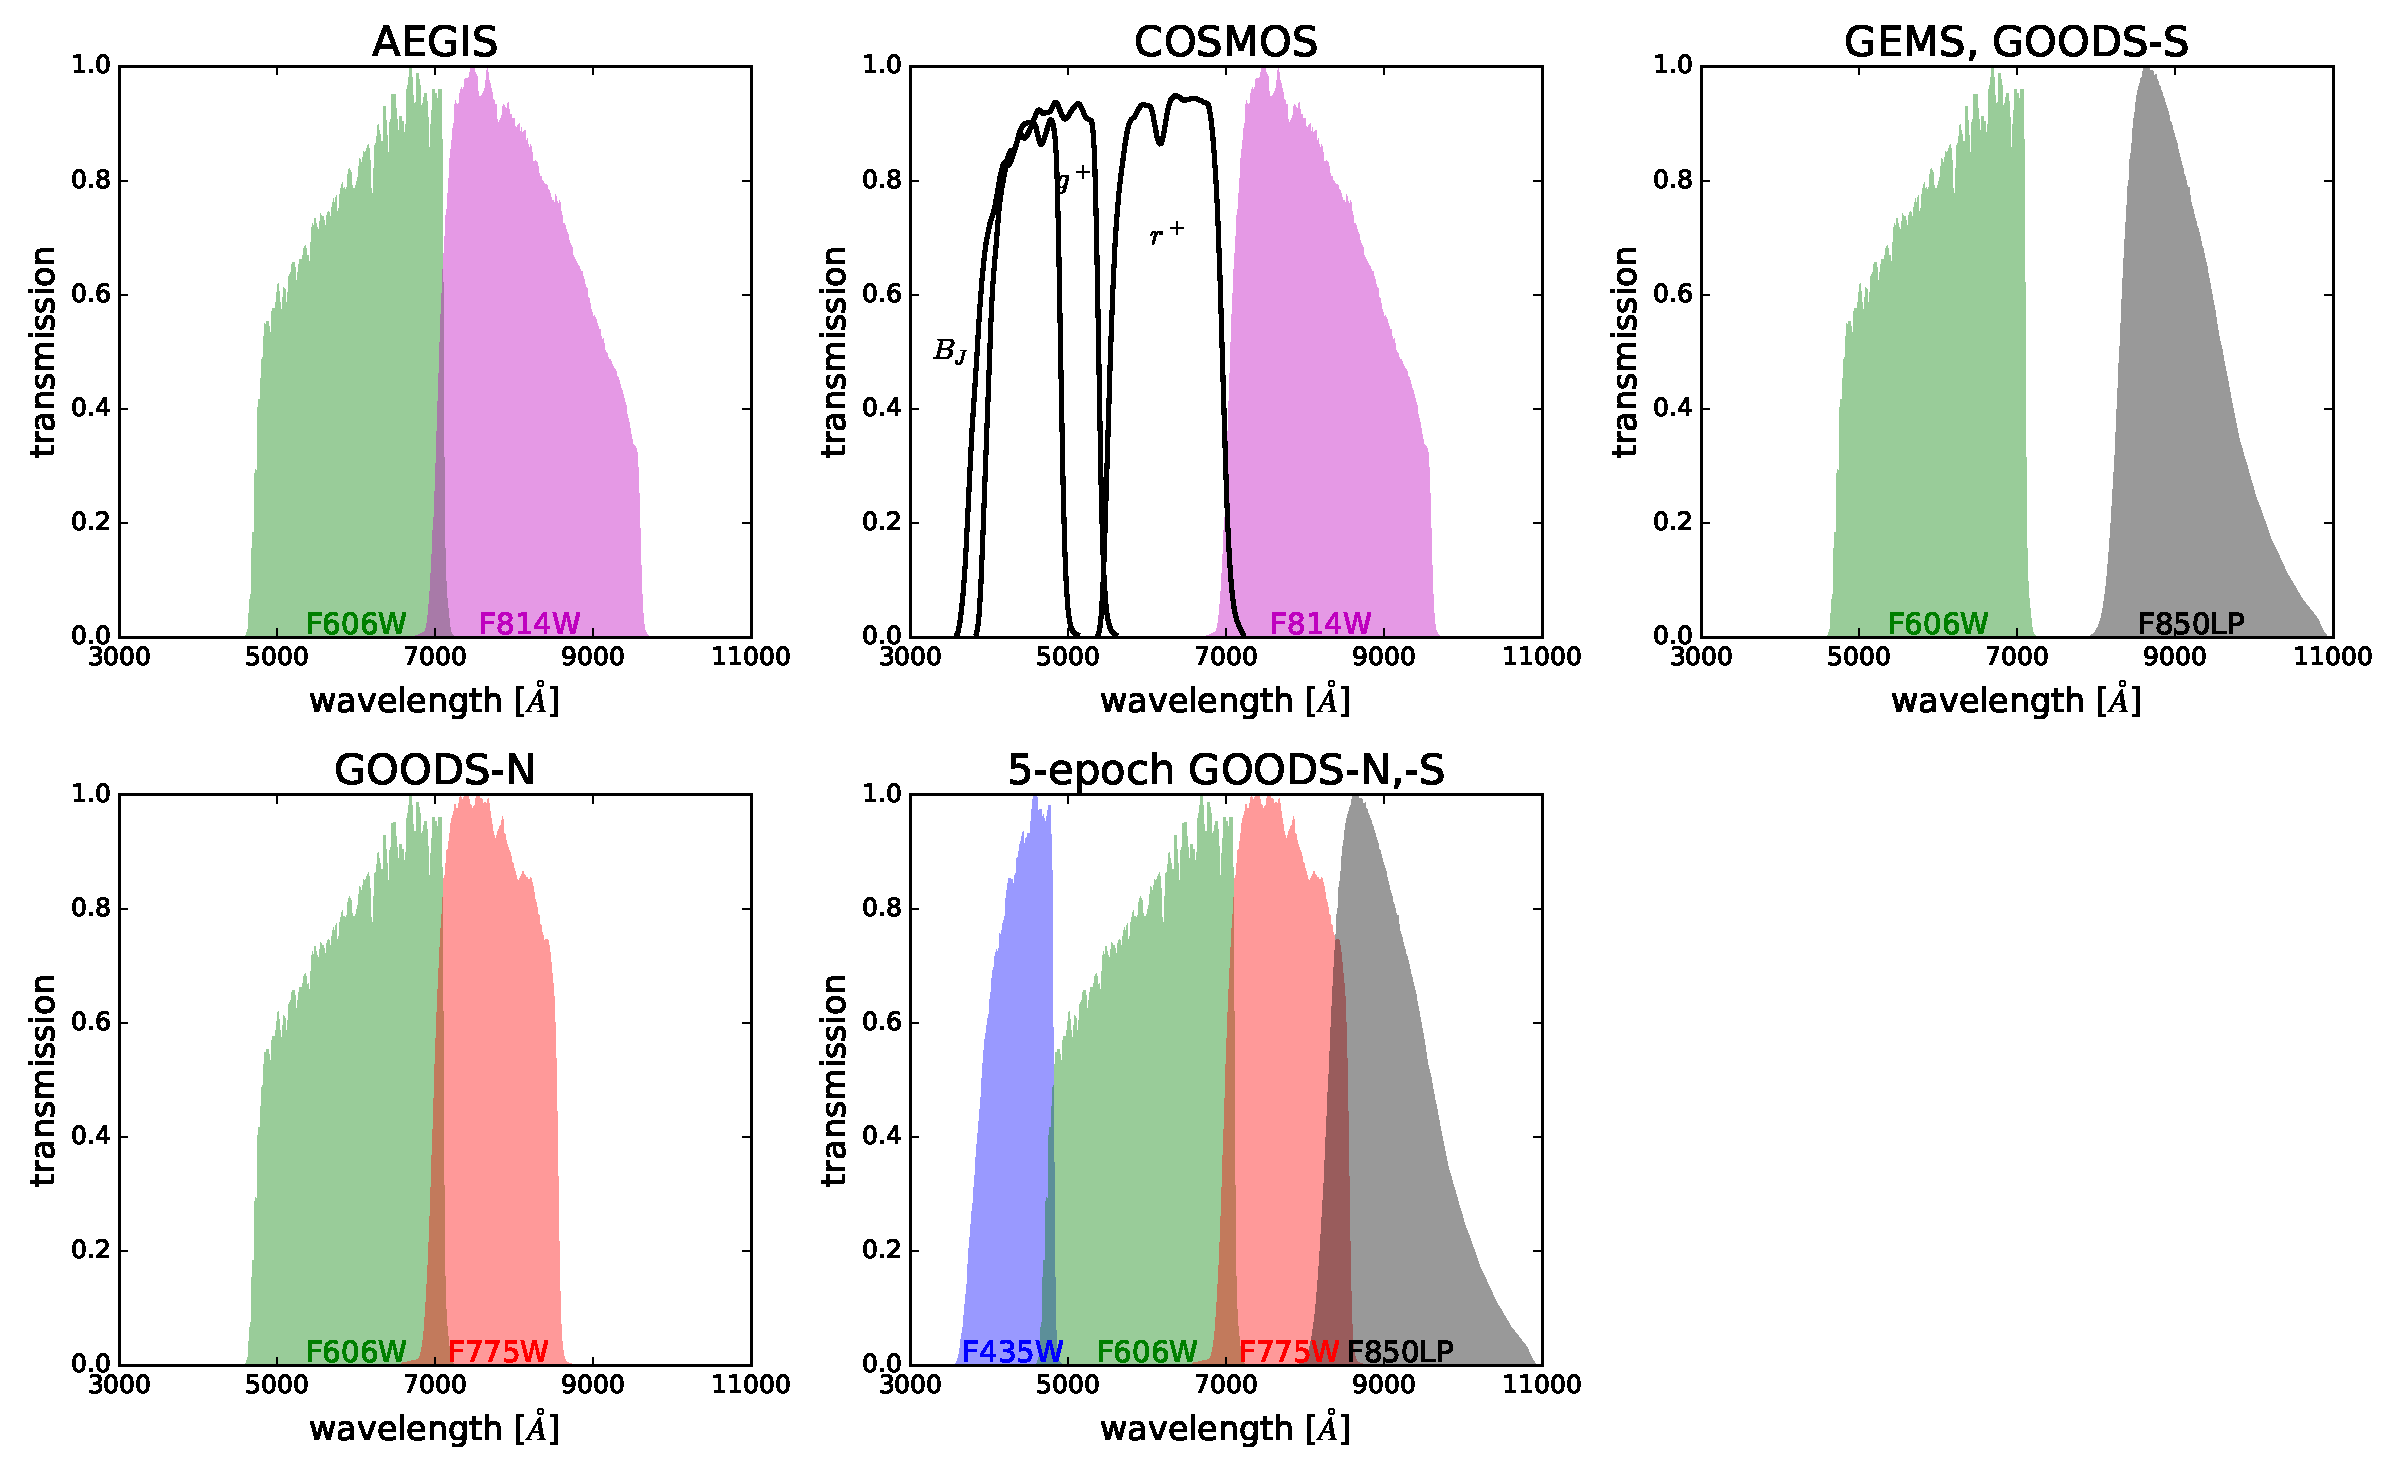
\includegraphics[width=160mm]{figures/filter_curves.pdf}
\caption{Transmission curves of the filters used by \textit{HST} Advanced Camera for Surveys (ACS) in wide-field channel mode for the various surveys in Galaxy Zoo: Hubble. The unfilled black curves show the filters for the Suprime Camera on the \textit{Subaru} telescope which were used to create color gradients in the composite images for COSMOS.\label{fig:filtercurves}}
\end{figure*}

Fake AGN

Stripe 82

Different treatment of colored noise in COSMOS; creating color gradients with Subaru data and using \Iband{} for illumination map.

FERENGI images.


\tabletypesize{\scriptsize}
\begin{deluxetable}{l|rr|rrr|rr|r|rr}

\centering
%\rotate
\tablecolumns{12}
\tablewidth{0pc}
\tablecaption{GZH redshifts by survey} 
\label{tbl:redshifts}
\tabletypesize{\scriptsize}
\tablehead{
 &   
\multicolumn{2}{c}{\underline{Griffith}} &
\multicolumn{3}{c}{\underline{3DHST}} &
\multicolumn{2}{c}{\underline{MUSYC}} &
\multicolumn{1}{c}{\underline{UltraVISTA}}&
\multicolumn{2}{c}{\underline{Total}} 
\\
\colhead{Survey} & 
\colhead{spec-z} & 
\colhead{photo-z} & 
\colhead{spec-z} & 
\colhead{grism-z} & 
\colhead{photo-z} & 
\colhead{spec-z} & 
\colhead{photo-z} & 
\colhead{photo-z} & 
\colhead{with redshift} &
\colhead{in survey}
}
\small
\startdata
%Survey     Gs        Gp    3ds    3dg     3dp       Ms      Mp       UVp       total
AEGIS    & 3,656  & 2,941  & 12  &  515  &  249    & 0     & 0     &  0      & 7,373  & 8,507\\
COSMOS   & 7,201  & 77,435 & 35  &  358  &  26     & 0     & 0     &  2,665  & 85,020 & 92,808 \\
GEMS     & 387    & 628    & 6   &  99   &  40     & 279   & 7,304 & 0       & 8,743  & 9,304\\
GOODS-N  & 1,947  & 37     & 418 & 1,545 &  1,381  & 0     & 0     & 0       & 5,328  & 12,030 \\
GOODS-S  & 1,080  & 4      & 327 & 1,348 &  281    & 816   & 1,184 & 0       & 5,040  & 10,284 \\
SDSS     & 0      & 0      & 0   &  0    &  0      & 0     & 0     & 0       & 37,545 & 51,861  \\
\hline
Total    & 14,271 & 81,045 & 798 & 3,865 & 1,977   & 1,095 & 8,488 & 2,665   & 114,204 & 184,794\\
\enddata
\end{deluxetable}

\subsection{Redshifts}

We compiled redshifts from a variety of sources to include in the GZH catalog. For each galaxy, the redshift selected is in the $\tt Z\_Best$ column of the data (see Table~\ref{tbl:catalog}), its type (spectroscopic: $\tt SPEC\_Z$, photometric: $\tt PHOTO\_Z$, or grism: $ \tt GRISM\_Z$) is listed in the column $\tt Z\_BEST\_TYPE$, and the source catalog ($\tt Griffith$ \citep{gri12}, $\tt 3DHST$ \citep{mom15}, $\tt MUSYC$ \citep{car10}, or $\tt UltraVISTA$ \citep{ilb13}) of the redshift is in column $\tt Z\_BEST\_SOURCE$.

For galaxies which have redshifts from multiple sources, we use the following algorithm to select the $\tt Z\_BEST$ redshift. We first prioritize spectroscopic redshifts; these are provided in the Griffith, 3DHST, and MUSYC catalogs. If a high quality spec-z exists in the Griffith catalog we use that, else 3DHST, else MUSYC. We show in Figure~\ref{fig:speczs} that over 98\% of the the spec-z's are consistent with each other, and therefore the priority order of selection makes no negligible difference. If no spectroscipic redshifts are available, we compare the 1-$\sigma$ errors of the photometric (Griffith, 3DHST, MUSYC, UltraVISTA) and grism (UltraVISTA) redshifts, and use the redshift with the smallest error. Table~\ref{tbl:redshifts} shows the results of this selection. 
 
\begin{figure*}
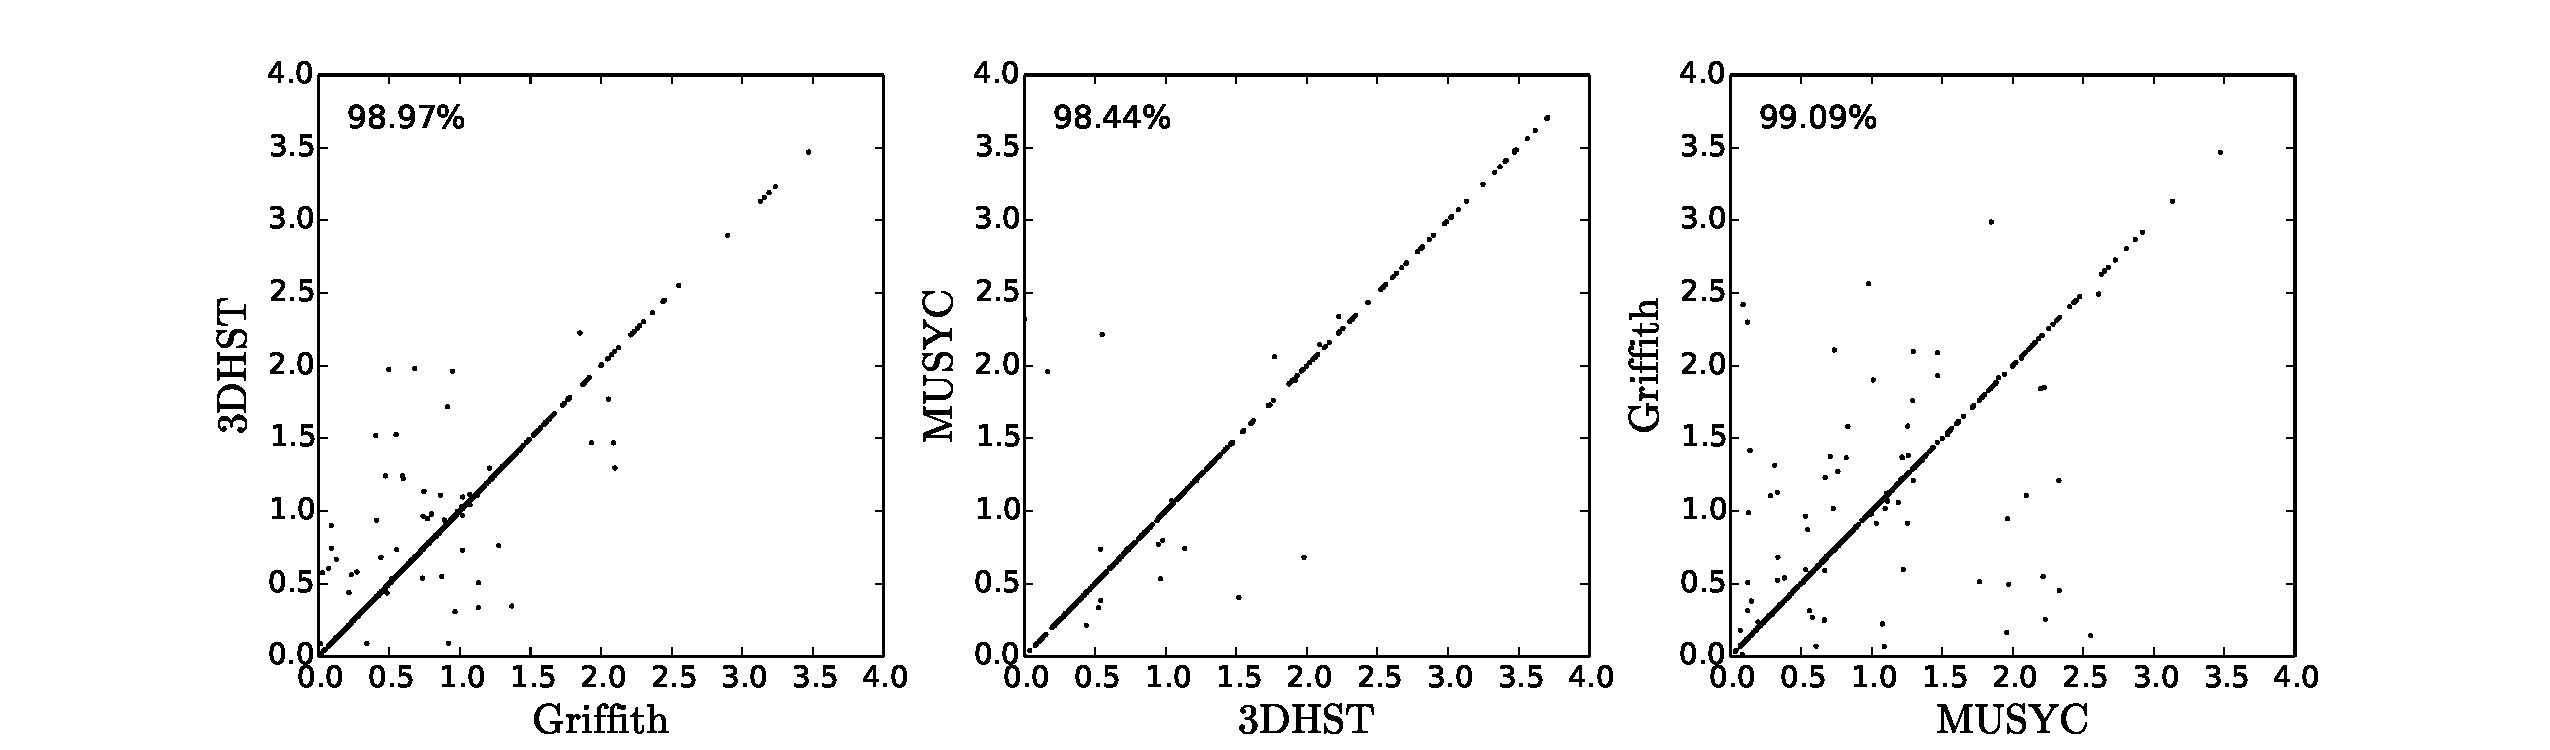
\includegraphics[width=160mm]{figures/specz_comparison.pdf}
\caption{Spectroscopic redshifts from Griffith, 3DHST, and MUSYC catalogs. The number in the upper left of each plot is the percentage of redshifts which agree within $\Delta z < 0.05$ between the two catalogs being compared in each panel. Within this range there is over 98\% agreement in redshifts between all three catalogs.}
\label{fig:speczs}
\end{figure*}



\subsection{User weighting}
\label{sec:weighting}
The votes of individual users who classified galaxies in GZH are combined to make a vote fraction for each question on the classification tree. Users' votes are weighted slightly \citep[in a method identical to that described in][]{wil13} such that users who frequently disagree with all other users end up having very low weights. The majority of users have weights very close to $w=1.0$ ({\bf STEVEN: Is this true for GZH - do you have a plot of the distribution of user weights or consistencies we can include here?}. 

\section{Galaxy Zoo interface and classifications}
\label{sec:gz_interface}

\begin{figure*}
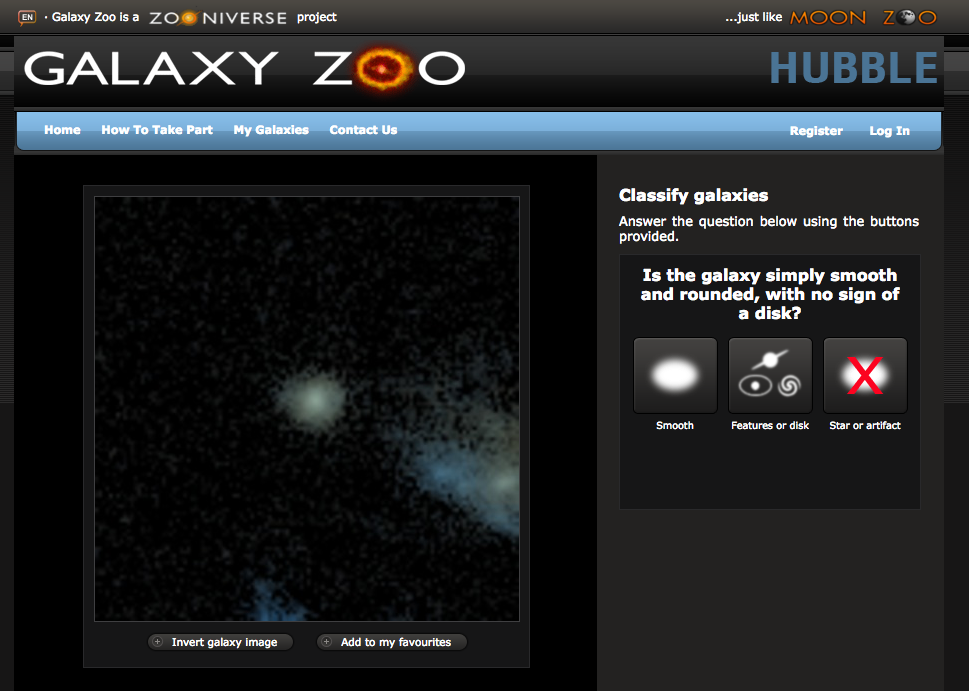
\includegraphics[width=160mm]{figures/gzh_interface.png}
\caption{Screenshot of the Galaxy Zoo: Hubble interface showing an example COSMOS image at the first step in the decision tree.\label{fig:interface}}
\end{figure*}

\section{Correcting for redshift-dependent classification bias}
\label{sec:debiasing}
The previous versions of Galaxy Zoo morphology classifications \citep{lin08,wil13} were based on observations of galaxies in the Sloan Digital Sky Survey (SDSS) which are typically at $z<0.1$. In these cases it was assumed that there was no cosmological evolution of the morphologies of galaxies and therefore any observed changes in the distribution of galaxies with different consensus morphologies was due to the effects of redshift on the image quality (\ie. the reduction in physical resolution, surface brightness dimming, etc). For both previous releases of GZ morphologies, we provided a correction for redshift-dependent bias based on matching the classification fractions at the highest redshfts with those at the lowest redshift. See \citet{bam09} and \citet{wil13} for the details. 

In the GZH samples, the redshift range is large enough that we expect to measure cosmological evolution of the types and morphologies of galaxies in the sample. As a result, the previous methods of correcting for redshift dependent bias will not work. In addition, the effects of band shifting will change the images even more across these redshift ranges. %Figure~\ref{fig:exampleFERENGI} illustrates some of the possible effects of losing features in spiral galaxies at high redshift. 

%-----------------------------------------------------------------------------------------------------------------------------------
%\begin{figure}
%\begin{center}
%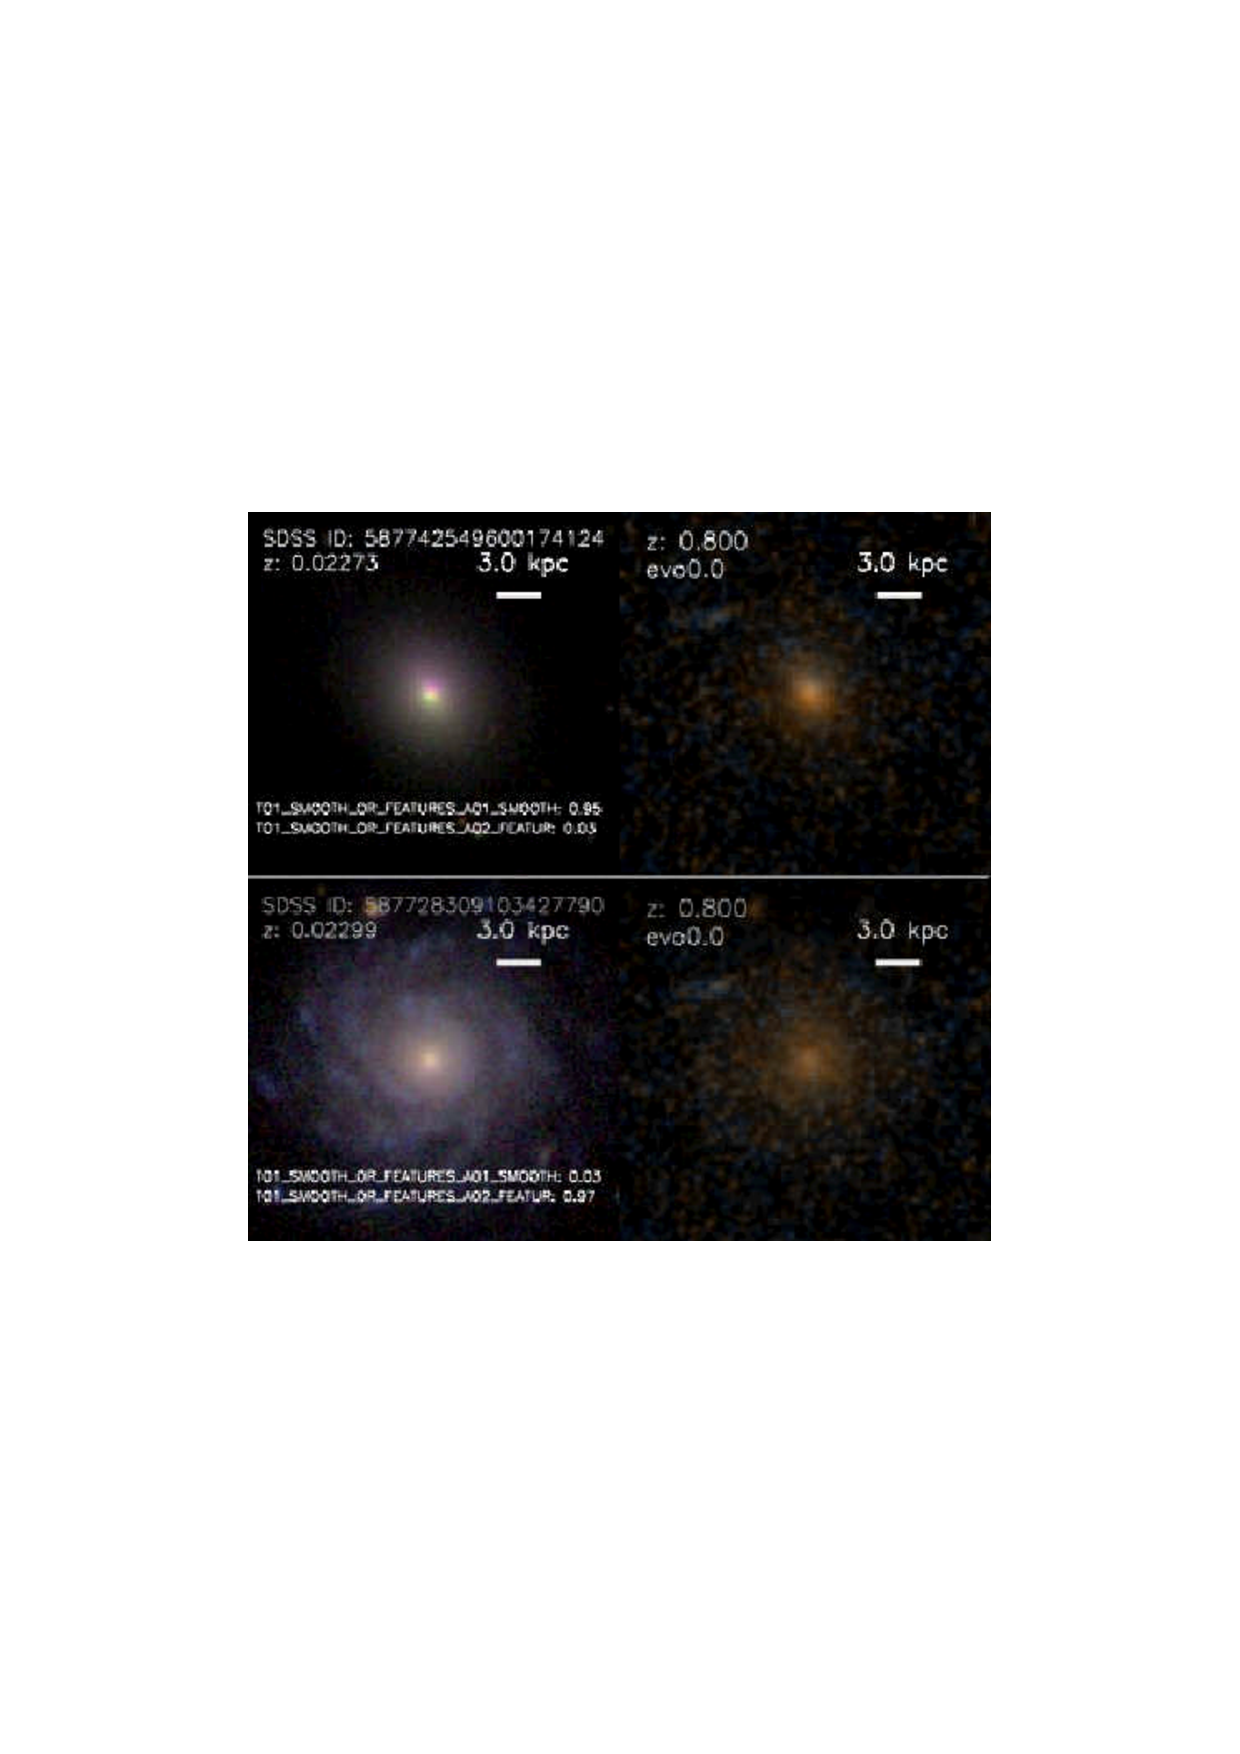
\includegraphics[width=60mm]{figures/example_ferengi2.pdf}
%\caption{Examples of an obvious spiral and obvious elliptical at $z=0$ which both look similar when redshifted to $z=0.8$. See below for the description of the method for redshifting.\label{fig:exampleFERENGI}}
%\end{center}
%\end{figure}
 %-----------------------------------------------------------------------------------------------------------------------------------

In order to test and correct for the effects of redshift, we generated a set of calibration images. These images consist of the same galaxy as it would appear over a variety of redshifts. The input images are from the SDSS \citep{yor00,str02} and are processed using the \ferengi{} code \citep{bar08a} to match the observational properties of the HST surveys out to $z=1$. These images were classified in the Galaxy Zoo interface using the same classification scheme as the original HST images.
 
\subsection{Selection of FERENGI input galaxies}

We selected 288 unique galaxies from SDSS imaging to run through the \ferengi{} code. The selection spanned a variety of galaxy morphologies (as selected by GZ2 classifications) and $r^\prime$-band surface brightnesses, and also spanned the redshift range of SDSS targets (in $N_z = 4$ bins) in order to be optimised for different target minimum redshifts in HST imaging. 

The selection criteria for the different morphological categories is summarised in Table \ref{morphologies}. The surface brightness selection ($N_\mu = 3$) was (1) low: $\mu > 21.5$~\magarc;  (2) mid: $20.5 < \mu < 21.5$~\magarc; and (3) high: $\mu < 20.5$~\magarc. For each of the four ``target redshifts'' ($z = 0.3, 0.5, 0.8$ and $1.0$), the images were redshifted in $\Delta z = 0.1$ bins up to $z=1.0$. 
 
\begin{table*}
\caption{Summary of morphological categories selected for FERENGI sample.\label{morphologies}}
\begin{tabular}{lllc}
\hline\hline
Morphology          & Label &  Selection                                                                                            & $N_{\rm objects}$ \\
                    &       &                                                                                                       & [$N_z \times N_\mu$] \\
\hline
Features            & Yes       & $p_{\rm features} > 0.8$, $p_{\rm odd} < 0.1$                                                         & 12 \\ 
                    & Int.      & $0.3 < p_{\rm smooth} < 0.6$, $p_{\rm odd} < 0.1$                                                     & 12 \\ 
                    & No        & $p_{\rm smooth} > 0.8$, $p_{\rm odd} < 0.1$                                                           & 12 \\ 
Merger              & No        & $p_{\rm features} > 0.8$, $p_{\rm odd < 0.1}$, $p_{\rm merger} < 0.1$                                 & 12 \\
                    & Int.      & $p_{\rm odd} > 0.5$, $0.1< p_{\rm merger} < 0.4$                                                      & 12 \\ 
                    & Yes       & $p_{\rm odd} > 0.5$, $p_{\rm merger} > 0.4$                                                           & 12 \\
Edge-on             & Yes       & $p_{\rm edgeon} > 0.8$, $p_{\rm features} > 0.5$                                                      & 12 \\
                    & Int.      & $0.4 < p_{\rm edgeon} < 0.8$ , $p_{\rm features} > 0.5$                                               & 12 \\
                    & No        & $p_{\rm edgeon} < 0.2$, $p_{\rm features} > 0.5$                                                      & 12 \\
Bar                 & No        & $p_{\rm bar} < 0.1$, $p_{\rm features} > 0.5$, $p_{\rm edgeon} < 0.2$                                 & 24 \\
                    & Int.      & $0.2 < p_{\rm bar} < 0.4$, $p_{\rm features} > 0.5$, $p_{\rm edgeon} < 0.2$                           & 24 \\
                    & Yes       & $p_{\rm bar} > 0.8$, $p_{\rm features} > 0.5$, $p_{\rm edgeon} < 0.2$                                 & 24 \\
Visible spiral      & No        & $p_{\rm spiral} < 0.2$, $p_{\rm features} > 0.5$, $p_{\rm edgeon} < 0.2$, $p_{\rm bar} < 0.1$         & 12 \\
                    & Int.      & $0.2 < p_{\rm spiral} < 0.8$, $p_{\rm features} > 0.5$, $p_{\rm edgeon} < 0.2$, $p_{\rm bar} < 0.1$   & 12 \\
                    & Yes       & $p_{\rm spiral} > 0.8$, $p_{\rm features} > 0.5$, $p_{\rm edgeon} < 0.2$, $p_{\rm bar} < 0.1$         & 12 \\
Oblique bulge size  & No        & $p_{\rm nobulge>0.6}$, $p_{\rm features} > 0.5$, $p_{\rm edgeon} < 0.5$, $p_{\rm bar} < 0.2$          & 12 \\
                    & Int.      & $p_{\rm justnoticeable}>0.6$, $p_{\rm features} > 0.5$, $p_{\rm edgeon} < 0.5$, $p_{\rm bar} < 0.2$   & 12 \\
                    & Yes       & $p_{\rm obvious|dominant}>0.5$, $p_{\rm features} > 0.5$, $p_{\rm edgeon} < 0.5$, $p_{\rm bar} < 0.2$ & 12 \\
Edge-on bulge shape & Round     & $p_{\rm rounded}>0.5$, $p_{\rm features} > 0.5$, $p_{\rm edgeon} > 0.5$                               & 12 \\
                    & Boxy      & $p_{\rm boxy}>0.4$, $p_{\rm features} > 0.5$, $p_{\rm edgeon} > 0.2$                                  & 12 \\
                    & No bulge  & $p_{\rm nobulge}>0.5$, $p_{\rm features} > 0.5$, $p_{\rm edgeon} > 0.5$                               & 12 \\
\hline\hline
\end{tabular}
\end{table*}

In addition to the physical parameters of the input images, the \ferengi{} output depends on assumptions of the global galaxy evolution model. This evolution is a crude mechanism that mimics the brightness increase of galaxies with increasing redshift (out to at least $z\sim1-2$). The effect on the redshifted images is simply an empirical addition to the magnitude of a galaxy of the form $M' = e\times z + M$, where $M'$ is the corrected magnitude, and $e$ is the evolutionary correction in magnitudes (i.e., $e=-1$ essentially brightens the galaxy by 1~magnitude by $z=1$). We ran \ferengi{} for values of $e$ starting from $e=0$ and decreasing to $e=-3.5$ in increments of $\Delta e = 0.5$. Figure~\ref{fig:exampleFERENGI} shows several examples of the effects of ``losing`` spiral/disc features with increasing redshift for two galaxies with $e=0$. 

The final number of \ferengi{} images produced for each galaxy is ultimately a function of galaxy's redshift, since the new images cannot be resampled at better angular resolution than the original SDSS data, as well as the number of $e$ values selected. Table~\ref{ferengivalues} summarizes the total sample of redshifted images produced for GZH. 

\begin{table}
\caption{Summary of FERENGI artificial redshifting \label{ferengivalues}}
\begin{tabular}{lccccr}
\hline\hline
$z_{\rm target}$ & $N_{z {\rm bins}}$ & $N_{\rm evolution}$ & $e_{\rm max}$ & $N_{\rm galaxies}$ & $N_{\rm images}$\\
\hline
0.3              & 8                  & 7                   & $-3.0$        & 72             & 4032 \\
0.5              & 6                  & 4                   & $-1.5$        & 72             & 1728 \\
0.8              & 3                  & 3                   & $-1.0$        & 72             &  648 \\
1.0              & 1                  & 3                   & $-1.0$        & 72             &  216 \\
\hline\hline
\end{tabular}
\end{table}

\begin{figure*}
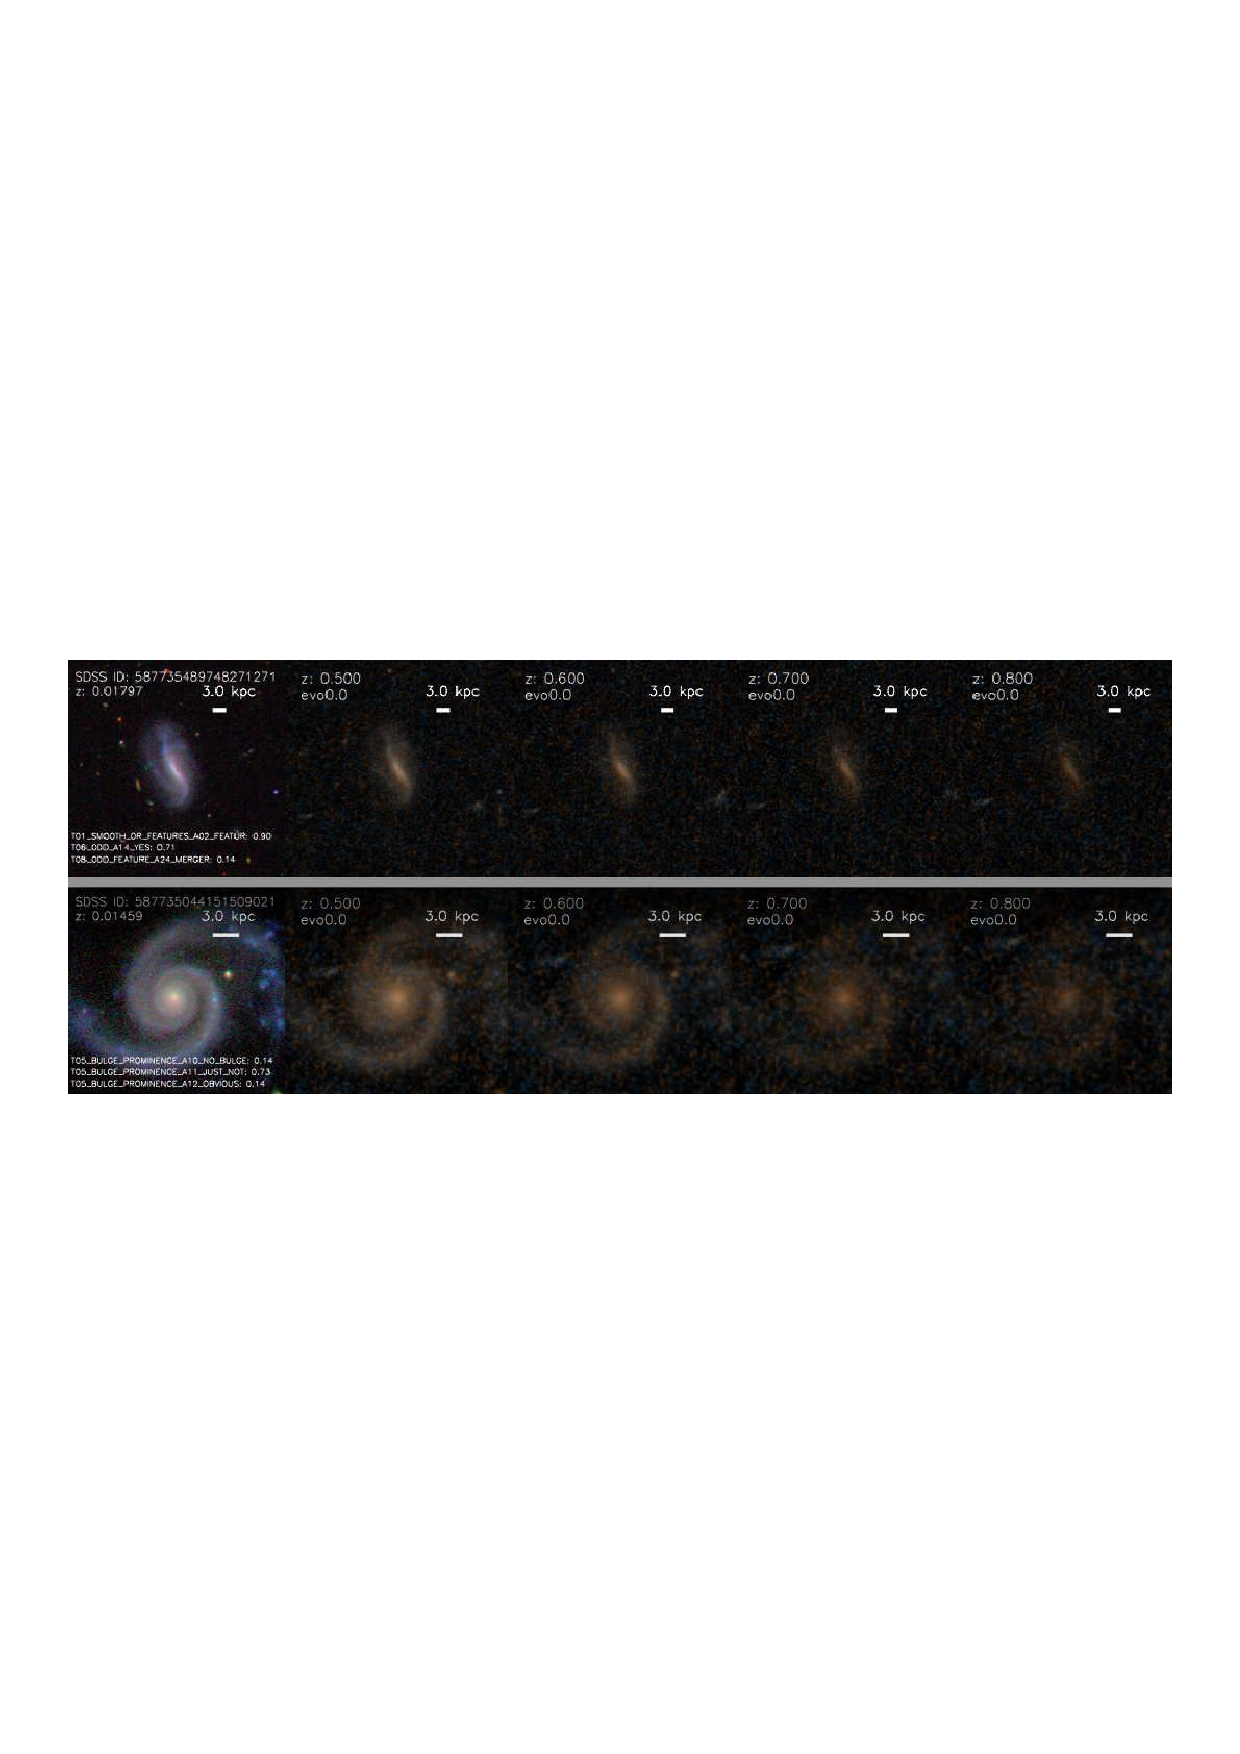
\includegraphics[width=160mm]{figures/example_ferengi.pdf}
\caption{Examples of two galaxies which have been run through the FERENGI code to produce simulated HST images. The value of $p_{\rm features}$ for each panel is (1) Top row: $p_{\rm features}=$ 0.9, 0.625, 0.35, 0.35, 0.225 and (2) Bottom row: $p_{\rm features}=$ 1.00, 0.875, 0.875, 0.625, 0.375. \label{fig:exampleFERENGI}}
\end{figure*}

\subsection{Correcting GZH morphologies for classification bias}
\label{sec:zeta}

The approach used in GZH for correcting the weighted classifications for user bias rests on the assumption that the \emph{amount} of bias is a function of the apparent size and brightness of the image as seen on screen. This is controlled by two types of parameters: \textbf{intrinsic} properties of the galaxy itself, such as its physical diameter and luminosity, and \textbf{extrinsic} properties, such as the distance (redshift) of the galaxy and its relative orientation. There are likely other parameters that affect user accuracy, such as the proximity of close companions \citep[``distraction bias''; see][]{joh15} or bias as a function of the individual user. The combination of all such parameters forms a high-dimensional space, and we have insufficient data to measure their individual effects. Instead, we use just two parameters that are intended to capture the bulk of the change in bias (based on GZ1/GZ2): a galaxy's $r^\prime$-band surface brightness ($\mu_r$; intrinsic) and redshift ($z$; extrinsic). 

The change in bias as a function of $\mu_r$ and $z$ is measured using the \ferengi{} images over all the evolutionary correction factors. We assume that the ``true'' (ie, debiased) vote fraction $f_{\mu,z}$ for a galaxy can be expressed as:

\begin{equation}
f_{\mu,z} = \left(f_{\mu,z=0.3}\right) \times e^{{\frac{z-z_0}{\zeta}}},
\label{eqn:fzeta}
\end{equation}

\noindent where $f_{\mu,z=0.3}$ is the ``calibrated'' vote fraction at the lowest redshift in the \ferengi{} bins ($z=0.3$) and $\zeta$ is a positive parameter that controls the rate at which $f$ decreases with increasing redshift. This formula fits the data relatively well (with almost no exceptions, the vote fractions for featured galaxies decrease monotonically with increasing redshift), and the exponential function bounds the observed vote fractions between $f_{\mu,z=0.3}$ and zero. Figure~\ref{fig:zeta_examples} show examples of the change in vote fraction and their fits to Equation~\ref{eqn:fzeta} for a random selection of galaxies in the \ferengi{} images. 

\begin{figure*}
\begin{center}
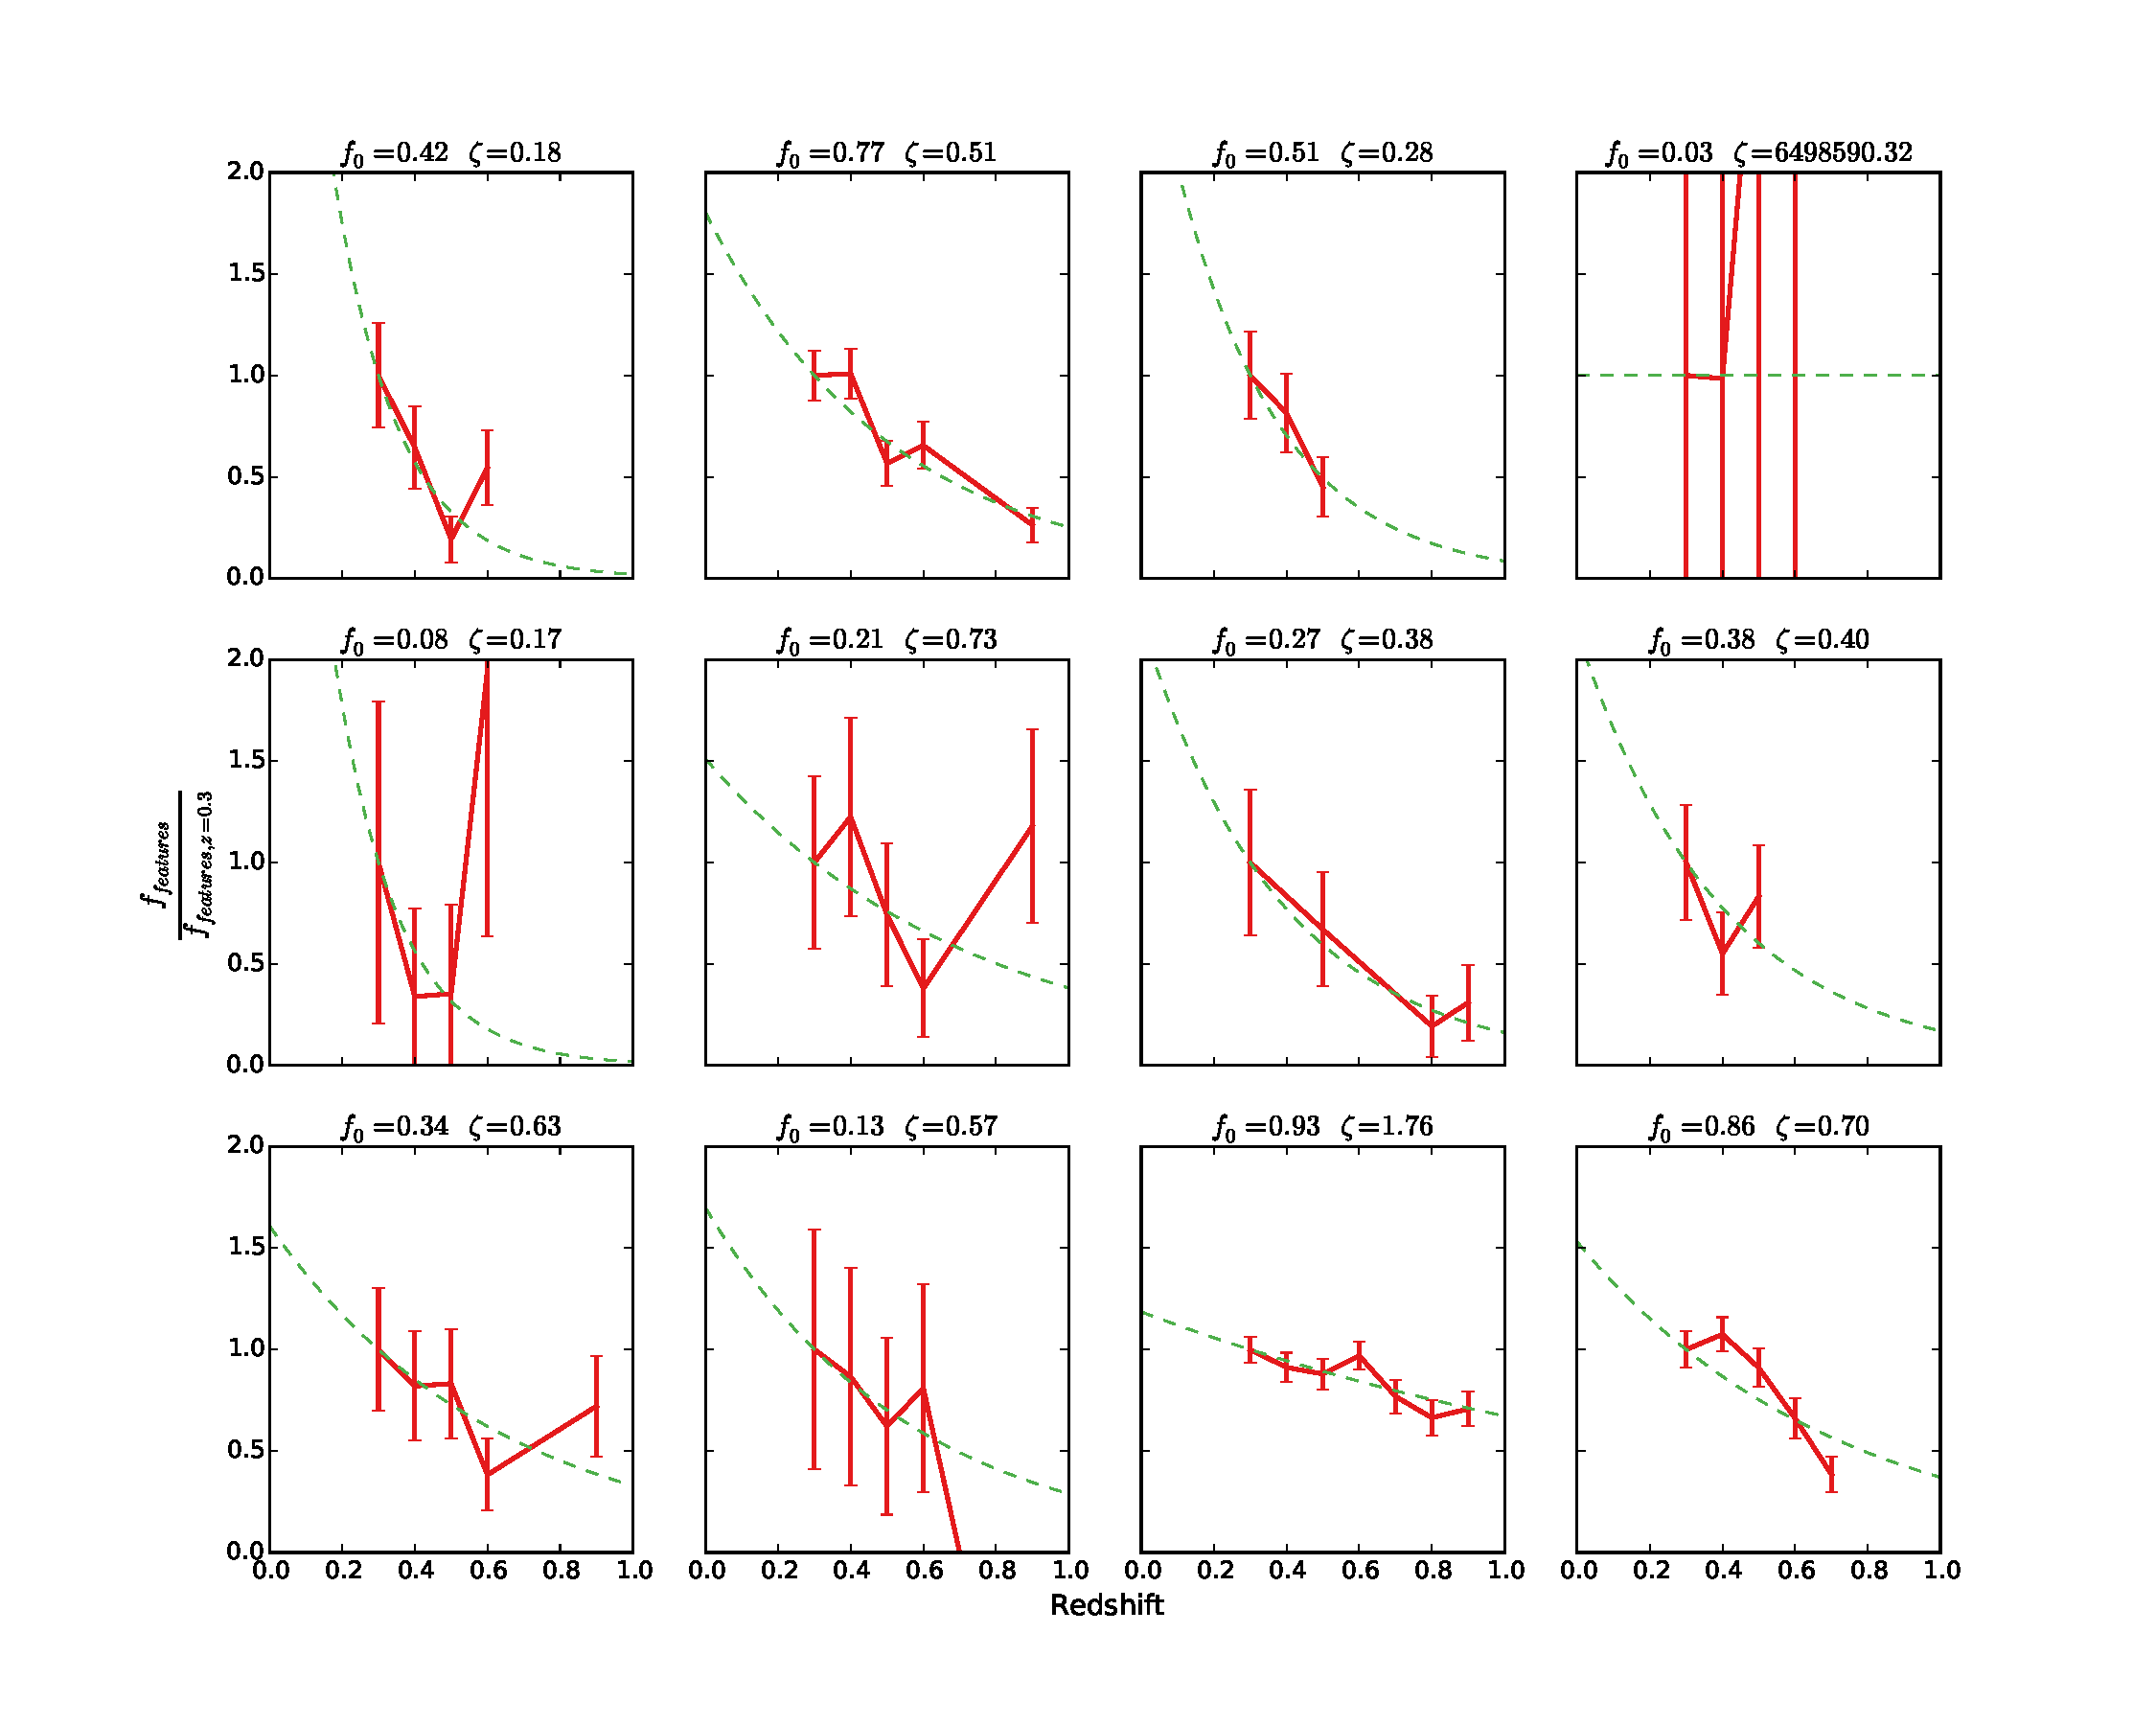
\includegraphics[width=\textwidth]{figures/zeta_examples.pdf}
\caption{Behavior of the normalized, weighted vote fractions of features visible in a galaxy ($f_\textrm{features}$) as a function of redshift in the artifical \ferengi{} images. Galaxies are a random selection of images with $e=0$ and at least three detectable images in redshift bins of $z\ge0.3$. The measured vote fractions (red points) are fit with an exponential function (Equation~\ref{eqn:fzeta}); the best-fit parameters are given above each plot. Error bars are Poissonian, assuming a median of 40~votes per galaxy.}
\label{fig:zeta_examples}
\end{center}
\end{figure*}

We use the values of $\zeta$ for \emph{all} sets of artifically redshifted galaxies to fit the overall distribution as a function of surface brightness, since we expect the correction being applied to vary as a function of the intrinsic galaxy properties. We restrict the galaxies that can be used to measure the calibration to those with data at the pivot redshift of $z=0.3$, non-zero $f_\textrm{features}$ at $z=0.3$, and with a reasonable fit to the exponential model ($\Delta \chi^2 > 3.0$). 

Figure~\ref{fig:zeta_mu} shows the results of fitting the \ferengi{} images with Equation~\ref{eqn:fzeta}; the correction is a weak function of galaxy surface brightness. Higher-surface brightness galaxies have stronger average corrections, likely because these galaxies are more likely to have larger $f_\textrm{features}$ values at high redshifts. Low surface brightness galaxies are more likely to begin low and remain low; the bounded nature of the dropoff (and Poissonian-like variance among the individual voters) means that the average magnitude of $\zeta$ will be less. 

\begin{figure}
\begin{center}
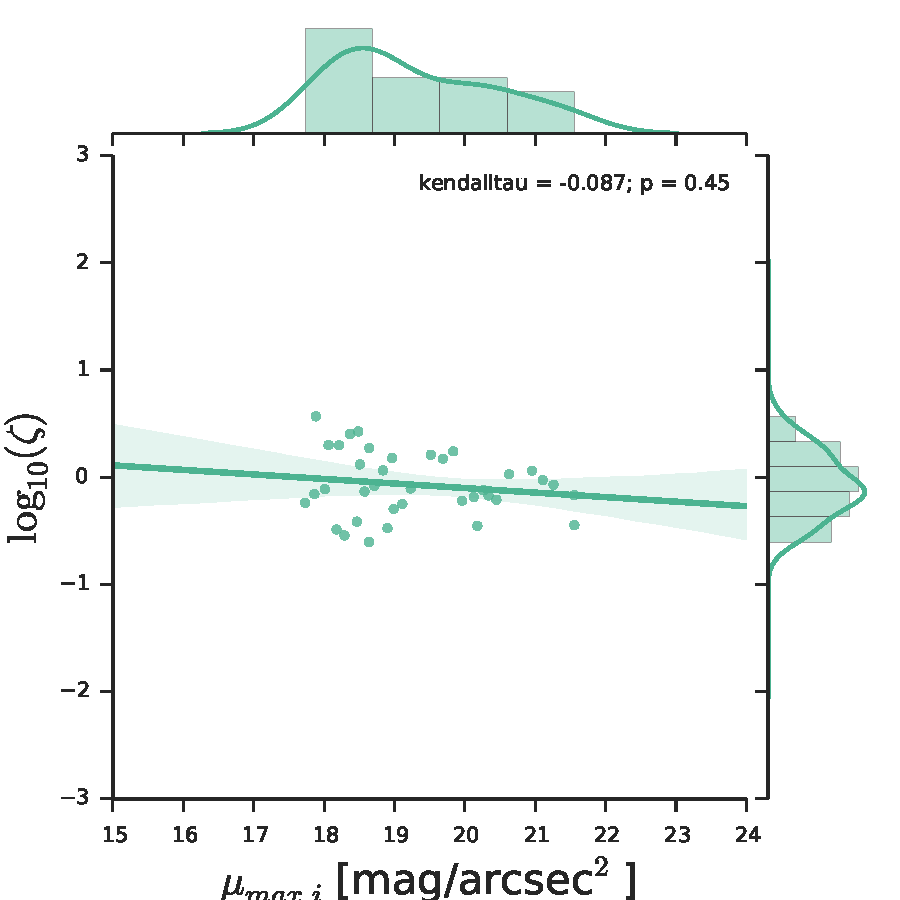
\includegraphics[width=0.50\textwidth]{figures/zeta_mu.pdf}
\caption{All fits for the vote fraction dropoff parameter $\zeta$ for $f_\textrm{features}$ in the \ferengi{} galaxies as a function of surface brightness. This includes only the 37~galaxies with a reasonably bounded range on the dropoff ($-10<\log(\zeta)<10$) and sufficient points to fit the function.}
\label{fig:zeta_mu}
\end{center}
\end{figure}

We fit the data in Figure~\ref{fig:zeta_mu} with a linear function such that:

\begin{equation}
\log_{10}(\hat\zeta) = \zeta_0 + \zeta_1 \times \mu,
\label{eqn:zetafit}
\end{equation}

\noindent where $\hat\zeta$ is the correction factor applied to each galaxy as a function of surface brightness. The best-fit parameters to the linear fit (from least-squares optimization) are $\zeta_0=0.1$, $\zeta_1=1.4$. To make the final debiased correction, we modify the simple exponential form of Equation~\ref{eqn:fzeta} to bound the debiased vote fractions between $f$ and 1:

\begin{equation}
f_\textrm{features,debiased} = 1 - (1 - f)e^{\frac{z-z_0}{\hat\zeta}}.
\label{eqn:fzeta_mod}
\end{equation}

\subsection{Results of $\zeta$ approach}\label{ssec:zeta_results}

\begin{figure}
\begin{center}
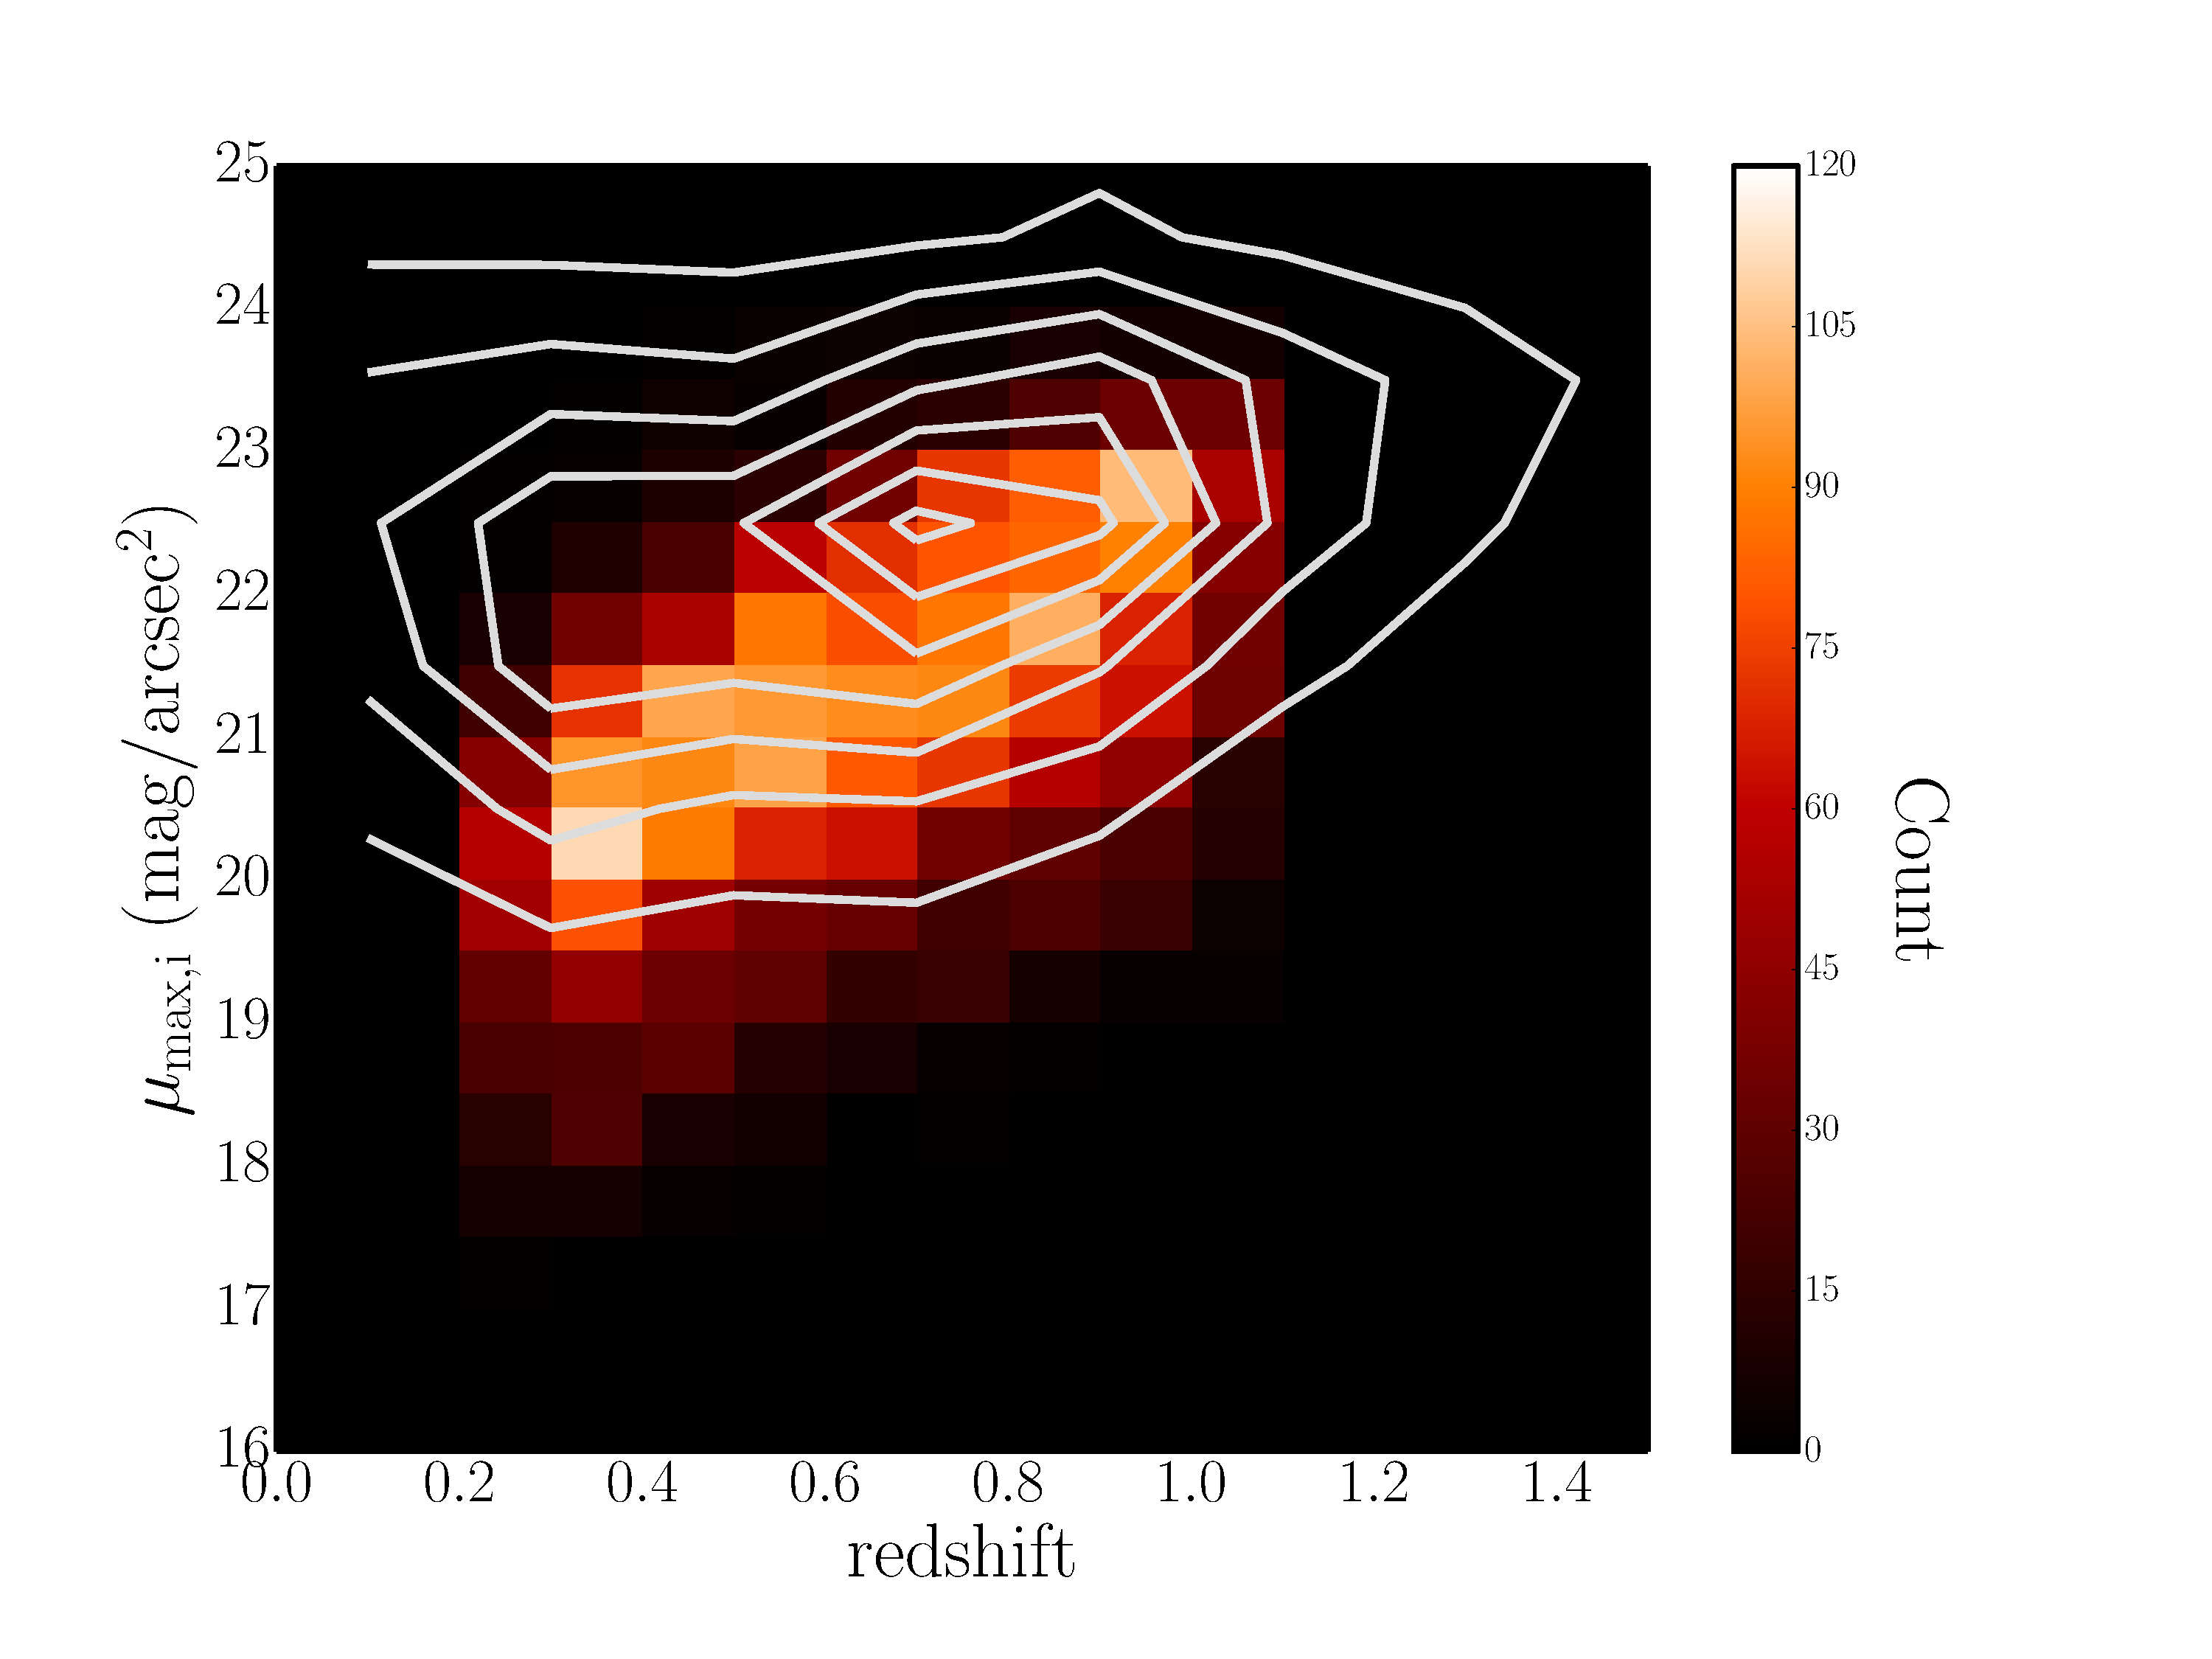
\includegraphics[width=0.5\textwidth]{figures/eye_of_sauron.pdf}
\caption{Surface brightness vs. redshift of 118,083 galaxies in the ACS sample. The white grid denotes the surface brightness and redshift range of the \ferengi{} images, subdivided in bins corresponding to fixed ranges used for analysis in Figure~\ref{fig:p_vs_p}.}

\label{fig:features_corrections}
\end{center}
\end{figure}

\begin{figure*}
\centering
\subfigure{[6a]\label{fig:6a}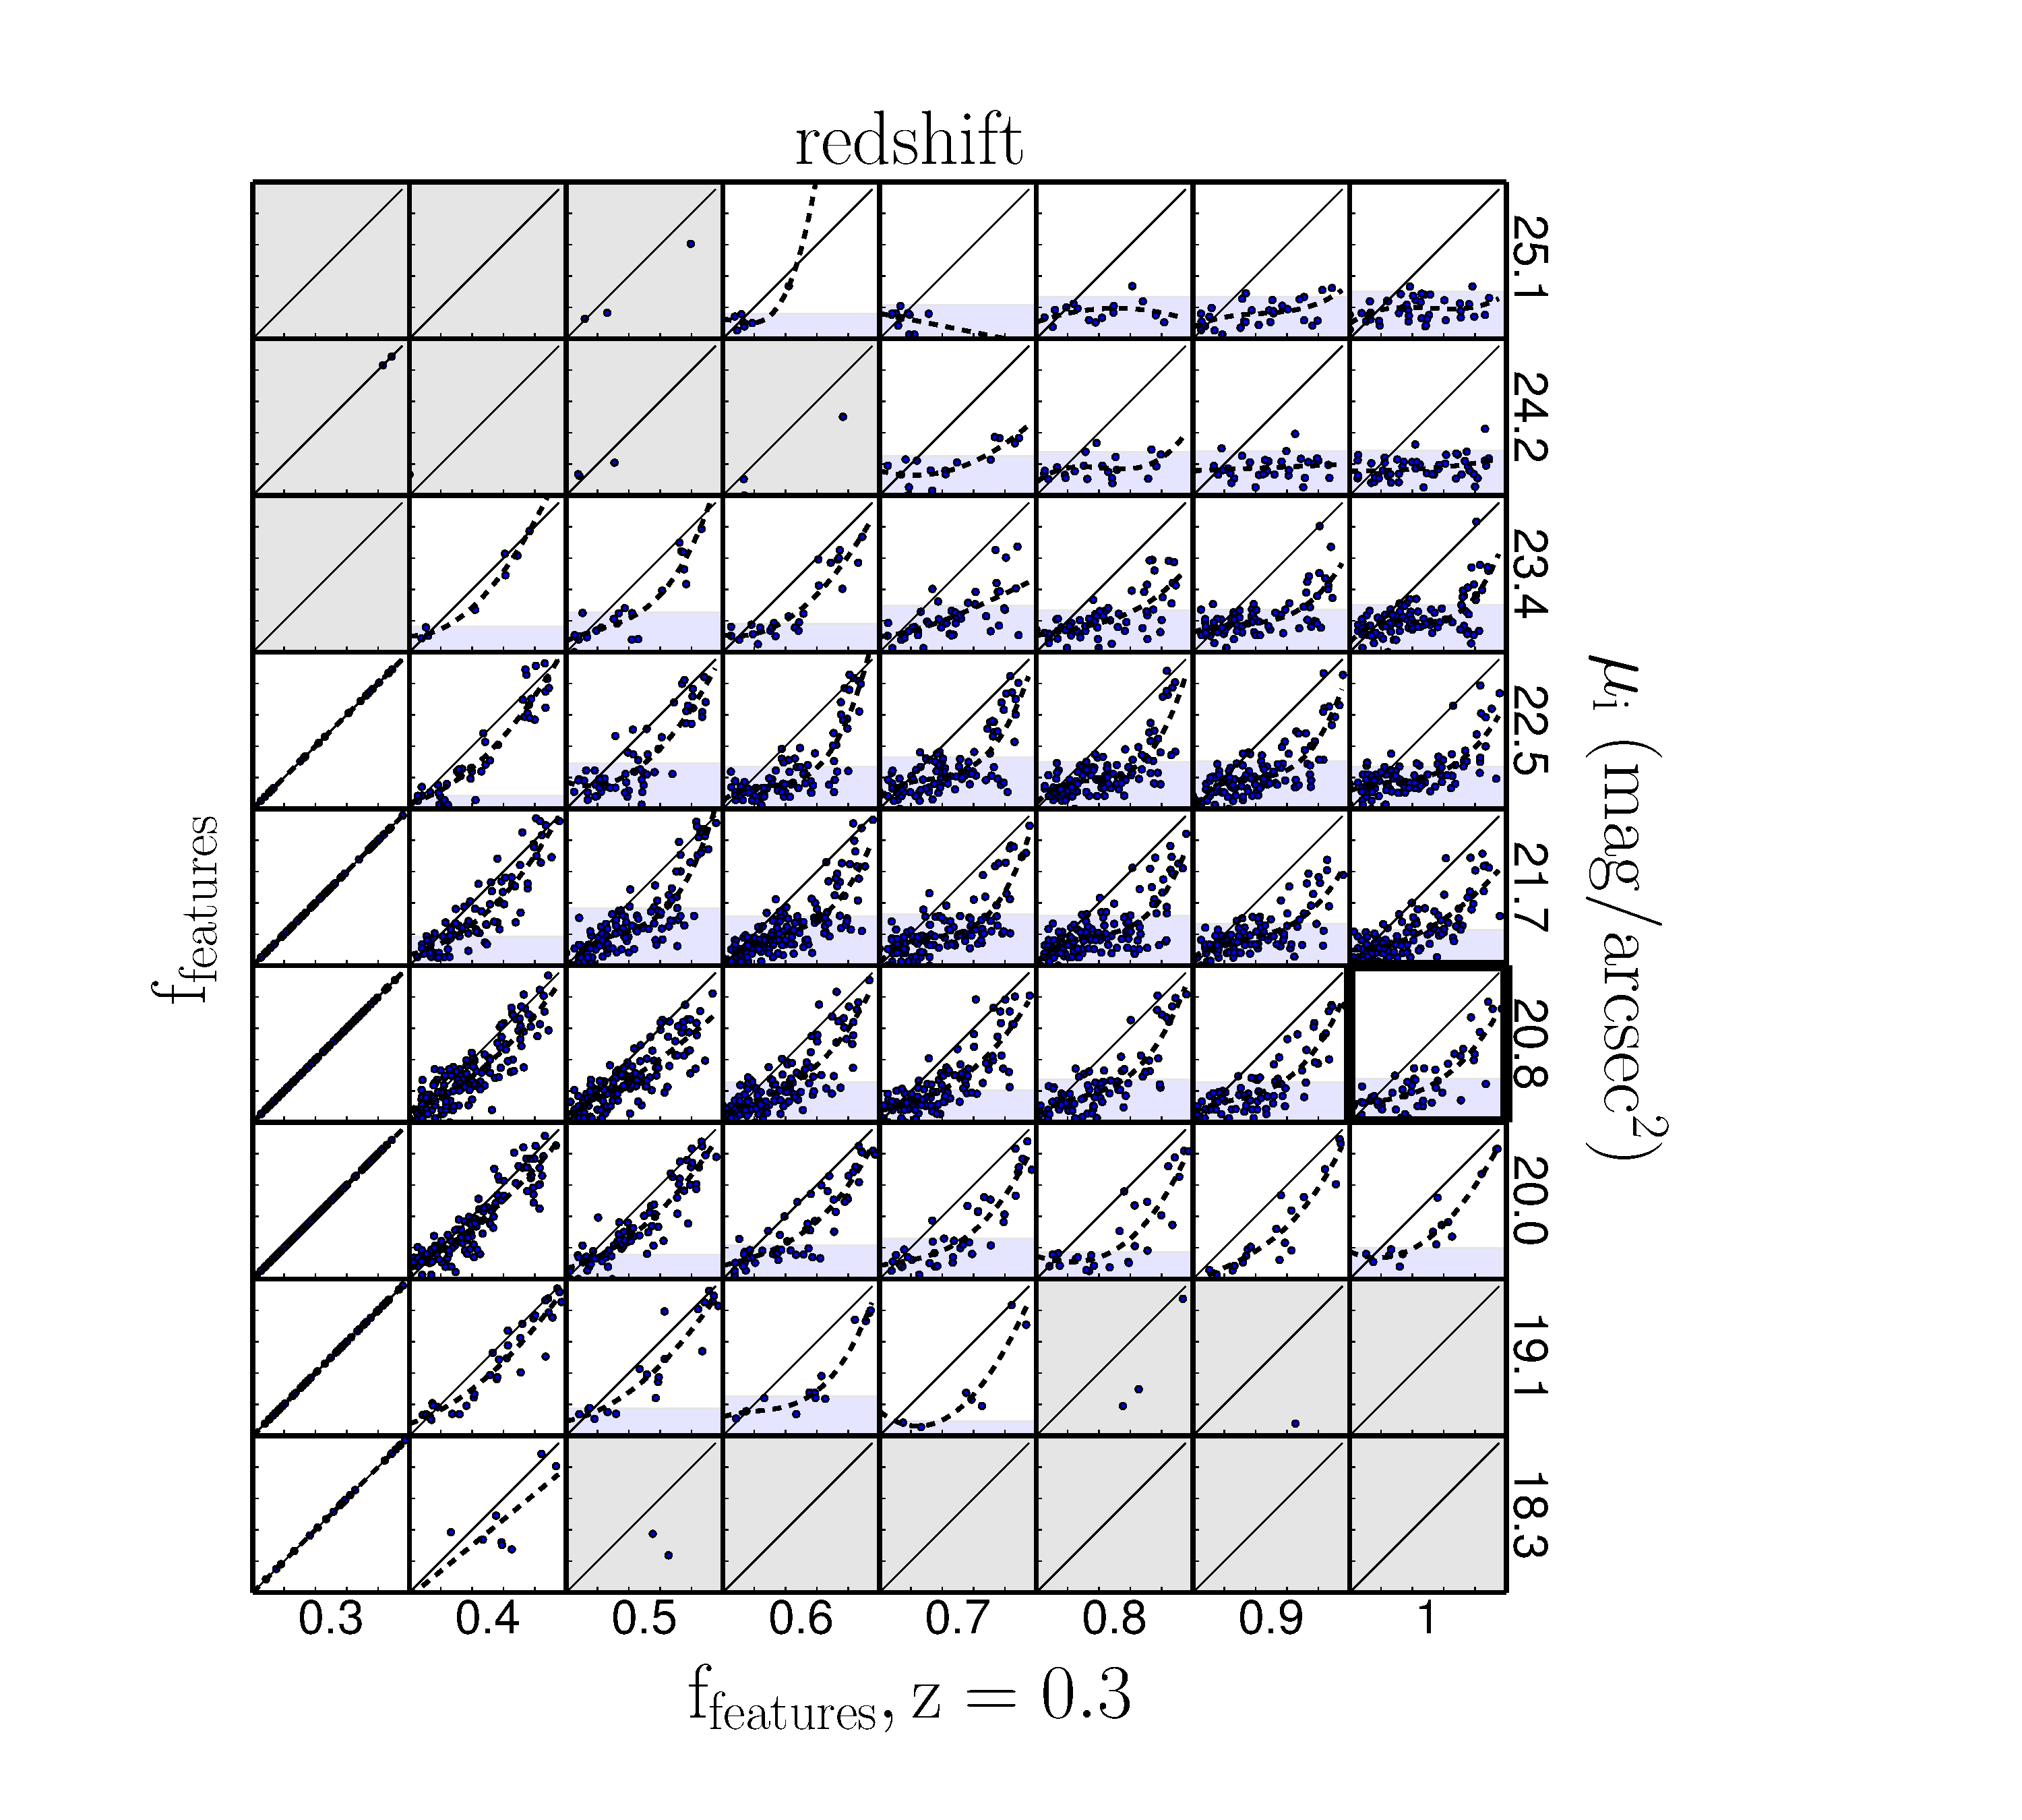
\includegraphics[width=0.5\textwidth]{figures/p_vs_p_SB_redshift.pdf}}
\subfigure{[6b]\label{fig:6b}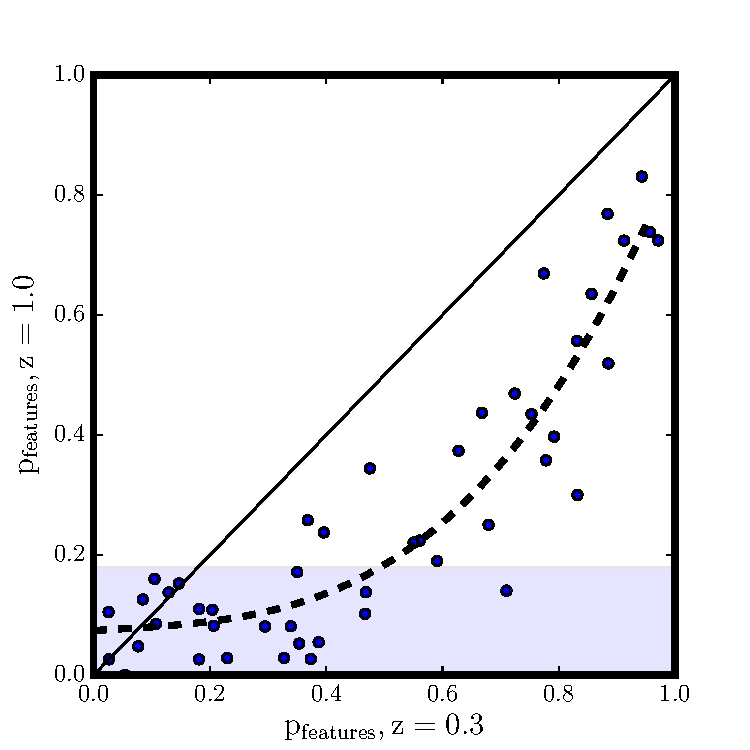
\includegraphics[width=0.4\textwidth]{figures/z1_mu20_subplot1.pdf}}
\\
\subfigure{[6c]\label{fig:6c}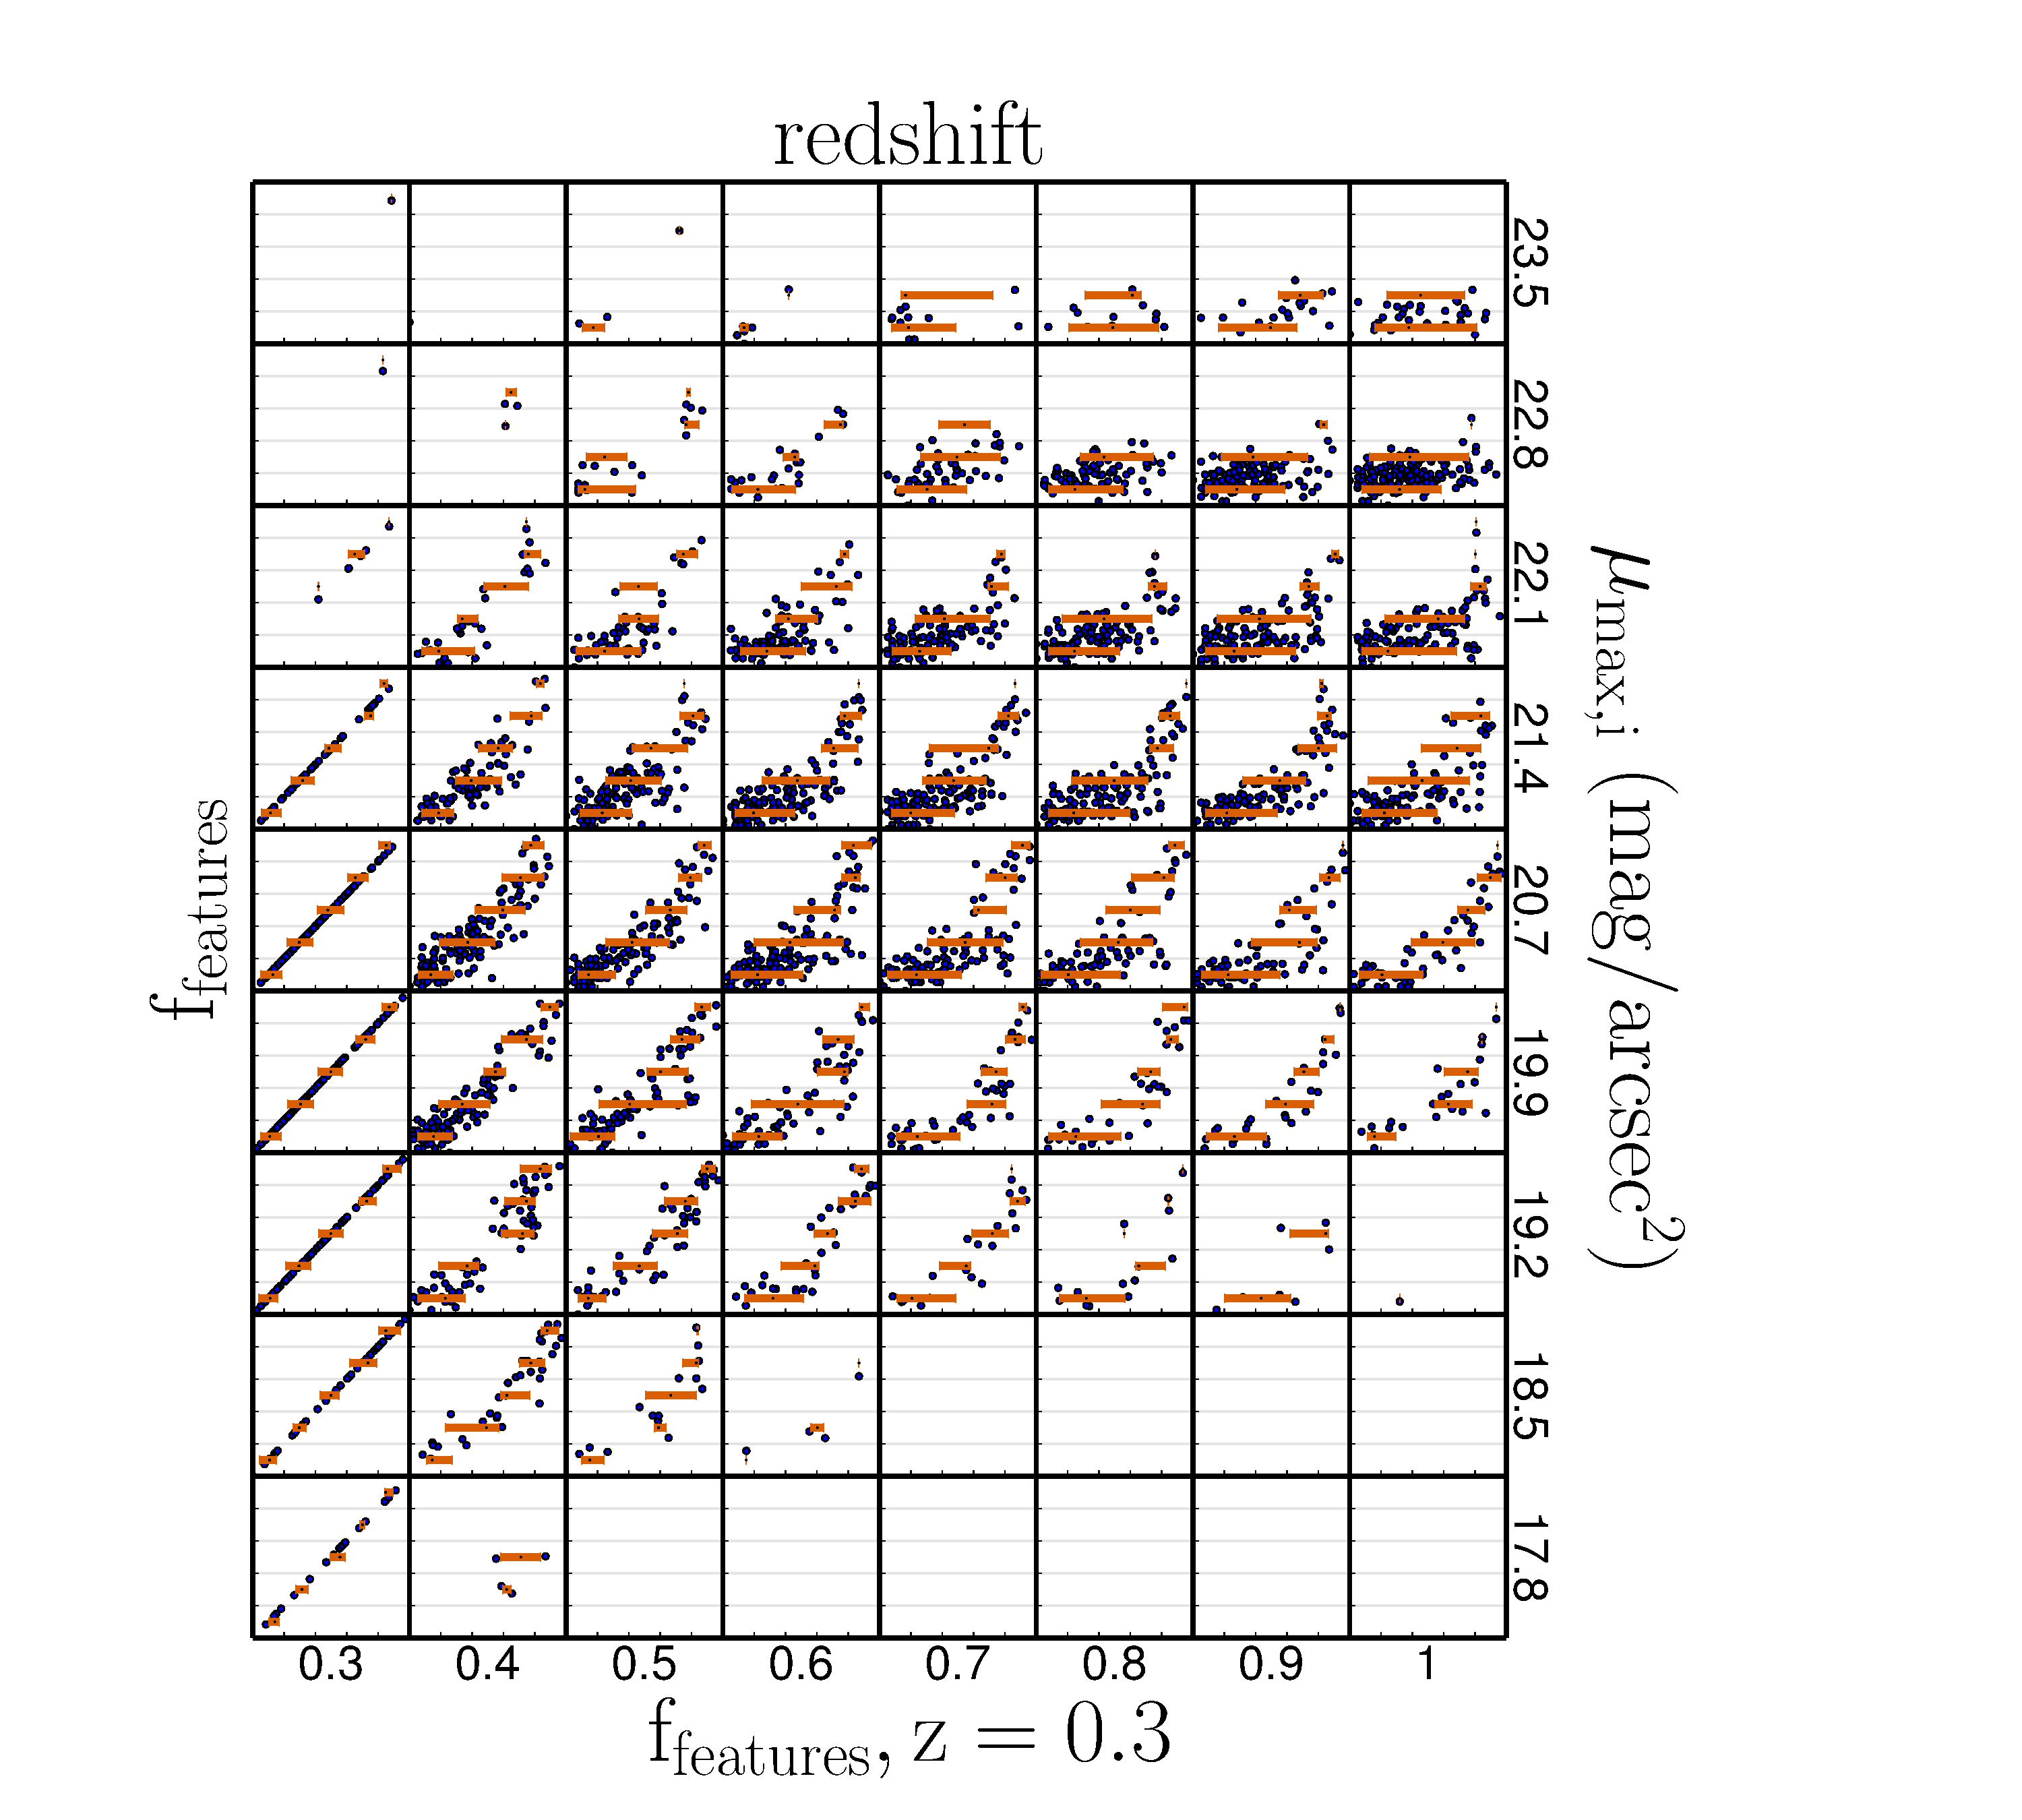
\includegraphics[width=0.5\textwidth]{figures/orangebars.pdf}}
\subfigure{[6d]\label{fig:6d}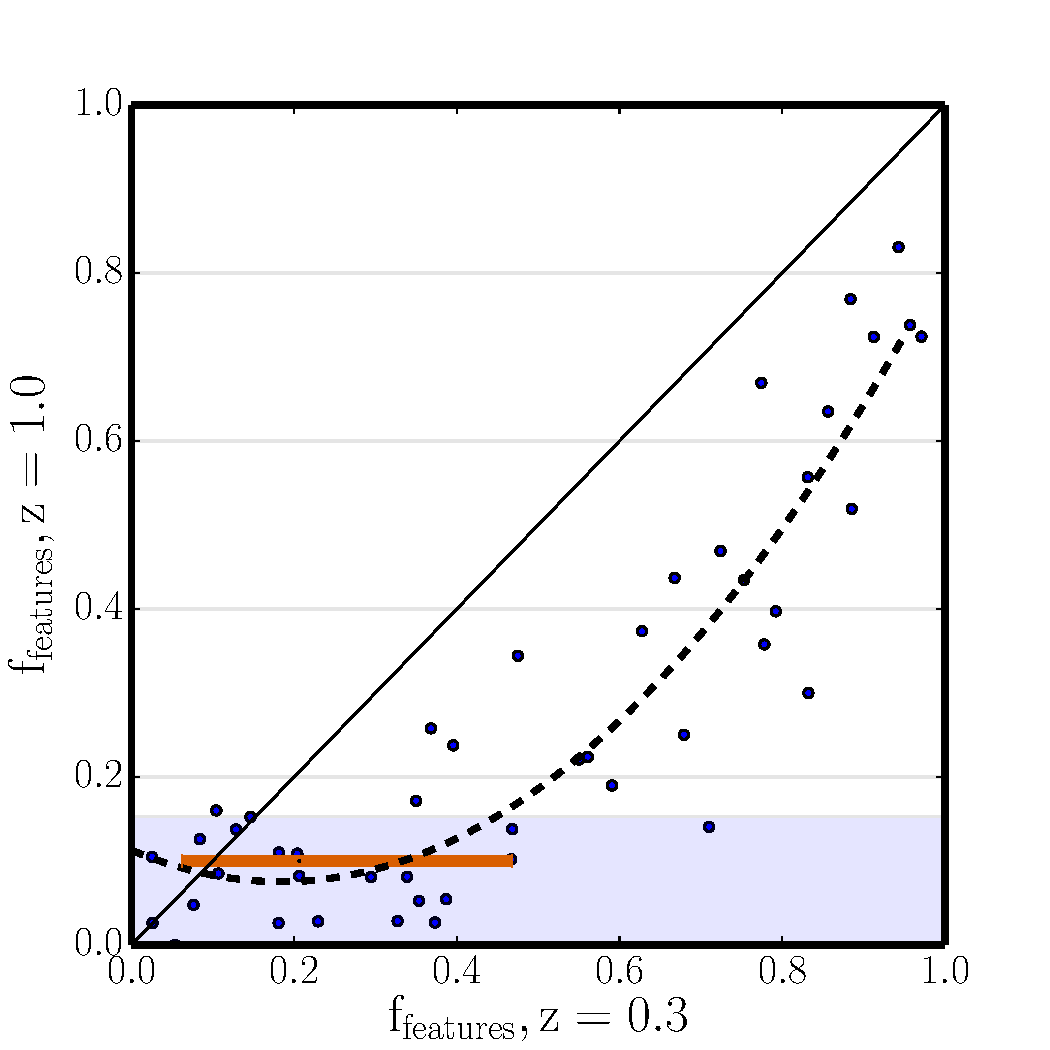
\includegraphics[width=0.4\textwidth]{figures/z1_mu20_subplot2.pdf}}
\caption{Effects of redshift bias in 3,950 images in the \ferengi{} sample. [6a]: Each point in a given redshift and surface brightness bin represents a unique galaxy. On the y-axis in each bin is the $p_{\rm features}$ value of the image of that galaxy redshifted to the value corresponding to that redshift bin. On the x-axis is the $p_{\rm features}$ value of the image of the same galaxy redshifted to $z=0.3$. The dashed black lines represent the best-fit polynomials to the data in each square. The solid black line represents $p_{\rm features,z}$ = $p_{\rm features,z=0.3}$. Regions in which there is a single-valued relationship between $p_{\rm features}$ at high redshift and at $z=0.3$ are white; those in which there is not are blue, and those with not enough data ($N<5$) are gray. [6b]: A larger version of the dark-outlined square in [6a], containing \ferengi{} galaxies that have been artificially redshifted to $z=1.0$ and have surface brightnesses between $20.3 < \mu < 21.0$ $\rm (mag/arcsec^2)$. [6c]: The same data as [6a] is shown. Each $z,\mu$ bin is divided into 4 sub-bins to determine the range of intrinsic $p_{\rm features,z=0.3}$ for a given range of observed $p_{\rm features,z}$ values. In each sub-bin, the orange bars represent the inner 80th percentiles of the data, the boundaries of which are the lower and upper limits of the debiased values. [6d]: The same data as [6b], but highlighting the upper and lower limit regions.}
\label{fig:p_vs_p}
\end{figure*}

In Figure~\ref{fig:p_vs_p} we examine the change in $p_{\rm features}$ for the \ferengi{} galaxies relative to their lowest simulated redshift. In this analysis, only galaxies whose lowest simulated redshift image was ($\rm z_{sim}=0.3$) were used (see Table \ref{ferengivalues}), and only those which had detectable surface brightness measurements in \sextractor{}; this includes 3,950 of the total 6,466 images. For each simulated redshift value $z$, and at a fixed surface brightness $\mu$, we plot $p_{\rm features,z}$, the value measured at that simulated redshift, vs $p_{\rm features,z=0.3}$, the value measured for the same galaxy imaged at $z=0.3$. 
 
Our objective is to use these data to predict, for a galaxy with a measured $p_{\rm features,z}$ value, what its $p_{\rm features}$ value \emph{would have been} if it had been viewed at $z=0.3$. This predicted value is defined as the debiased vote fraction $p_{\rm features,debiased}$, and is calculated by applying a correction to the measured value of $p_{\rm features}$, determined by the $\zeta$ function described in the previous section. A reliable predicted value can be obtained so long as the relationship between $p_{\rm features,z}$ and $p_{\rm features,z=0.3}$ is single-valued; that is, for a given $p_{\rm features,z}$, there is exactly one corresponding value of $p_{\rm features}$ at $z=0.3$. 

Figure~\ref{fig:p_vs_p} shows that the relationship between $p_{\rm features,z}$ and $p_{\rm features,z=0.3}$ is \emph{not} always single valued; hence, it is not appropriate to correct galaxies that lie in certain regions of surface brightness/redshift/$p_{\rm features}$ space. These regions tend to have low $p_{\rm features}$ values at high redshift, but a wide range of values at $z=0.3$. These regions contain two morphological types of galaxies: First are genuine ellipticals, which have low values of $p_{\rm features}$ at both high and low redshift. Second are disks whose features become washed out at high redshift; hence their $p_{\rm features}$ value at $z=0.3$ may be quite high, while the value observed at high redshift is very low. This effect is strongest at high $z$ and low $\mu$, where features become nearly impossible to discern in the images.

Our criteria for determining whether a region of this space is single-valued, and therefore correctable, is as follows: In each surface brightness and redshift bin, we model the relationship between $p_{\rm features,z}$ and $p_{\rm features,z=0.3}$ by fitting the data with a polynomials of degrees 3, 2, and 1, and use the best fit out of the three. These fits are shown as the dashed black lines in Figure~\ref{fig:6a}. Any flat regions of the polynomial fits are areas in which there is not a clear single-valued relationship between $p_{\rm features,z}$ and $p_{\rm features,z=0.3}$; we quantify this by setting a minimum slope cut of 0.4. Any data in which the polynomial fit has a slope less than this value is considered \emph{not} one-to-one, and therefore ``uncorrectable.'' These regions are highlighted in blue in figure ~\ref{fig:6a}. Uncolored (white) regions of the plot have sufficiently high slopes for us to consider the relationship to be single-valued; galaxies in these regions are considered ``correctable'', and only these are used in measuring the parameters for the $\zeta$ function (Section \ref{sec:zeta}). Only surface brightness/redshift bins with at least 5 galaxies were considered; regions with fewer than 5 galaxies we consider to have ``not enough information'' to determine the  $p_{\rm features,z}$ and $p_{\rm features,z=0.3}$ relationship, these are colored gray in Figure~\ref{fig:6a}.

The unshaded regions in Figure~\ref{fig:6a} define discrete ranges of redshift, surface brightness, and $\pfeatures$ a galaxy must have in order for the $\zeta$ approach to be confidentely applied to a galaxy in the GZH sample. While the appropriate correctable regions were defined discretely, we assume the true correctable region is a smooth function of z, $\mu$, and $\pfeatures$. To define this smooth space, we use a convex hull method to enclose the correctable and uncorrectable \ferengi{} galaxies is z-$\mu$-$\pfeatures$ space. Due to scatter, the boundaries of the resulting hulls overlap. The boundaries are then adjusted until the contamination from both groups is minimized. We use the resulting hulls to define the correctable and uncorrectable regions for categorizing the Hubble galaxies. The results of this method and final categorization of the Hubble sample is displayed in Table~\ref{tbl:hubble_debiasable}. We find that of the galaxies at redshift higher than $z=z_{0}=0.3$, 17\% of these are able to be debiased using the $\zeta$ method, 27\% cannot be debiased, and 56\% cannot be determined, due to a lack of redshift or information or due to a lack of \ferengi{} data corresponding to those galaxies' redshift/surface brightness values.

For the ``uncorrectable'' galaxies, those for which we cannot confidentely assign a single debiased $p_{\rm features}$ value, we instead determine a likely \emph{range} of debiased values, using a method visualized in Figure~\ref{fig:6c}. Here we again use the \ferengi{} simulated data to analyze the range of intrinsic $p_{\rm features,z=0.3}$ values for any given observed $p_{\rm features}$ value, again as a function of surface brightness and redshift. In each z,$\mu$ bin, we examine the spread of intrinsic values of $p_{\rm features,z=0.3}$ for 4 ranges of observed $p_{\rm features}$. We quantify the range of intrinsic values as the inner 80\% of the data; this range is represented by the orange bars in Figure~\ref{fig:6c}. For any galaxy which can't be directly debiased by the $\zeta$ method, then, we use these ranges to denote the upper and lower limits on what we expect $p_{features,z=0.3}$ to be for any observed value of $p_{\rm features}$. 


\begin{table}ー
\caption{Distribution of \ferengi{} images analysed in Figure~\ref{fig:p_vs_p}. Correctable images had a single-valued relationship between their measured $p_{\rm features}$ values at high and low redshifts (white regions in Figure~\ref{fig:p_vs_p}). Uncorrectable images had a non single-valued relationship (blue regions). NEI images had undetermined relationships due to a lack of data ($N<5$) in their corresponding z-$\mu$ bins (gray regions).   \label{ferengi_corrections}}
\begin{tabular}{lrr}
\hline \hline
				                   & N       & \% \\
\hline 
Correctable                        & 1,884   & 48\% \\
Uncorrectable                      & 1,986   & 50\% \\
NEI                                & 80     &  2\%\\
Total                              & 3,950   & 100\% \\
\hline \hline
\end{tabular}
\end{table}

\subsection{Challenges of debiasing questions beyond ``smooth or features''}
Each FERENGI image does not have the same number of users answering each question, due to the structure of the decision tree. Every user answers the first question, ``Is the galaxy smooth and rounded, with no sign of a disk?''; as such the vote fractions $\rm p_{smooth}, p_{features}$, and $\rm p_{artifact}$ are all computed with the minimum statistical error for any question, with roughly 40 total answers (see Section~\ref{sec:gz_interface}). The number of users to answer any subsequent question, however, is always equal to or less than the number to answer the preceding question. For this reason, some galaxies may have very few (or even zero) answers to a question further down the tree (see Figure make-figure-of-count-distribution-for-each-question). To minimize statistical error in computing vote fractions, a cut on the number of answers to a given question is always implemented. 

In the FERENGI data, we find that this places large limitations on the amount of information we can extract for the higher order questions. We require that at least 5 users answer each question for a galaxy image at $z=0.3$ \emph{and} its image at higher $z$. This requirement placed on both images is not met by a significant number of galaxies for questions beyond question 1. Without sufficient galaxies in each surface brightness/redshift bin, we cannot accurately measure a relationship between vote fractions and redshift; for this reason we only offer debiased vote fractions for question 1. \textbf{perhaps compute number of galaxies that can be fit to zeta for each question, show a table? overkill?} In Section \ref{sec:ferengi_bar} we show results of an attempt to measure $\zeta$ for $\rm p_{bar}$. 

\begin{itemize}
\item talk about where the Hubble sample falls in this space, reference table \ref{tbl:hubble_debiasable} 
\item justify $N>5$ and spread $< 0.2$ (or find a better way to choose criteria)
\item check out corrections for correctable and NEI, show some sample images of corrected galaxies
\item show some data for $\pbar$, determine or justify why we won't debiase them  
\end{itemize}

 
\begin{table*}
\caption{Breakdown of what we can correct out of the GZH data, by sample.  \emph{updated from 3-8-16: Switching to full depth for all GOODS data. Shallow depth information in appendix.}\label{tbl:hubble_debiasable}}
\begin{tabular}{lcrrrrrrr}
\hline\hline
                                   & Correction type & AEGIS   & COSMOS & GEMS & GOODS-N & GOODS-S    & SDSS    & Total \\
\hline
Correctable                        & 0               & 1,654   & 15,170 & 1,837 & 993    & 835     	& 0       & 20,489\\
Uncorrectable                      & 1               & 1,917   & 26,113 & 2,423 & 1,385  & 1,282   	& 0       & 33,120\\
No Correction Needed ($z \le 0.3$) & 2               & 955     & 11,926 & 1,175 & 415    & 400     	& 37,545  & 52,416\\ 
NEI                                & 3               & 2,847   & 34,511 & 3,308 & 2,535  & 2,523   	& 0       & 45,724\\
No Redshift Information            & 4               & 1,134   & 5,088  & 561   & 687    & 102   		& 14,316  & 21,888\\
Total                              &                 & 8,507   & 92,808 & 9,304 & 6,015  & 5,142   	& 51,861  & 173,637\\
\hline\hline
\end{tabular}
\end{table*}

\begin{figure*}
\begin{center}
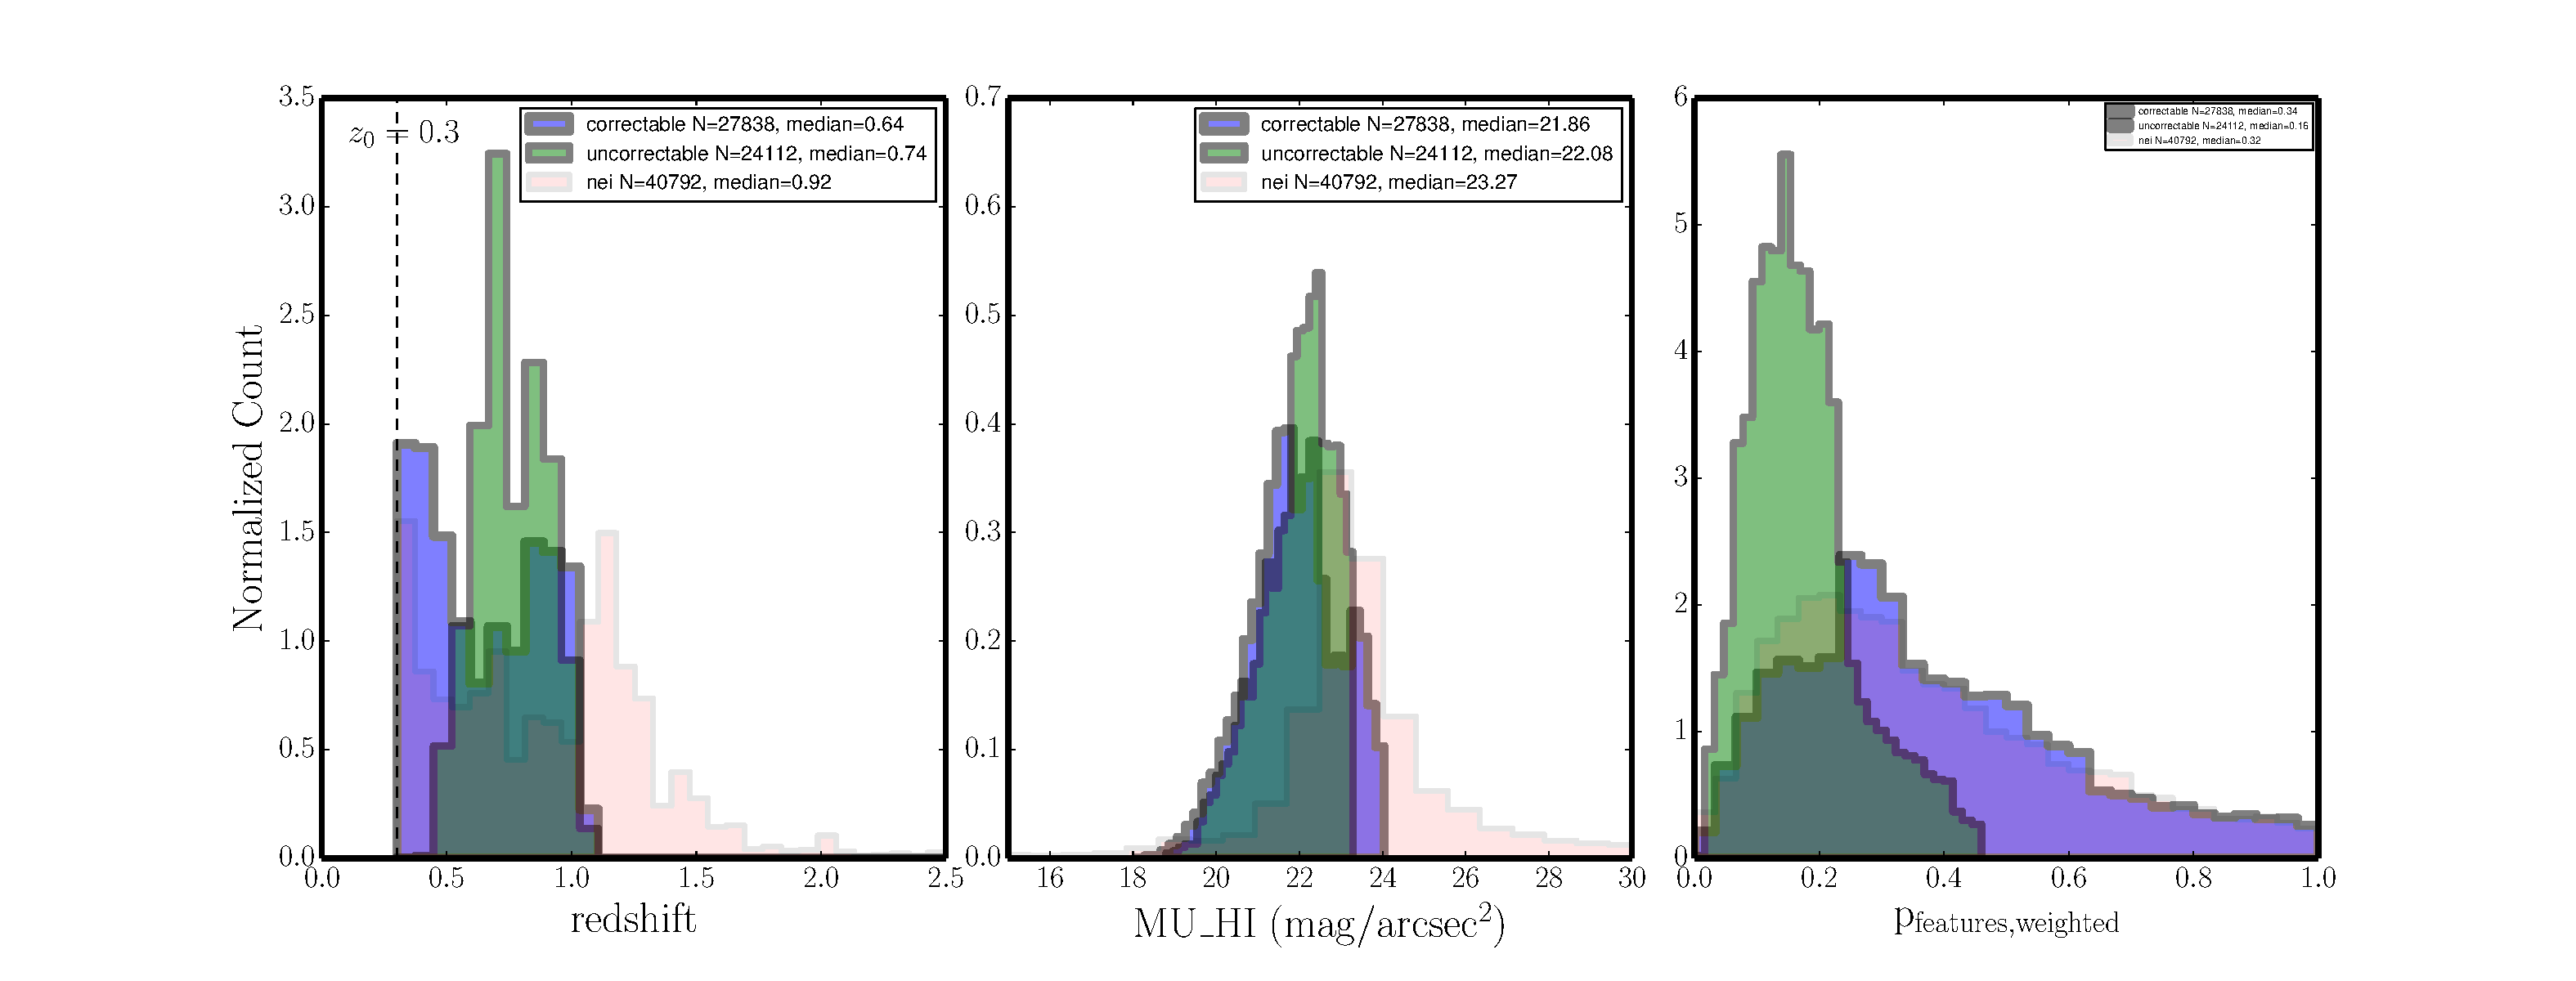
\includegraphics[width=\textwidth]{figures/hubble_z_mu_p_distributions.pdf}
\caption{Distributions of redshift, surface brightness, and $p_{features}$ for correctable (purple), uncorrectable (green), and NEI (pink) galaxies in the full GZH sample. The uncorrectable galaxies tend towards higher redshift, slightly lower in surface brightness, and lower values of $p_{features}$ than the correctable galaxies. The long tail of NEI galaxies in redshift and surface brightness demonstrates the limits of the \ferengi{} sample, for which there is no data at $z>1$ or $\mu>24$.}
\label{fig:z_mu_p}
\end{center}
\end{figure*}

\begin{figure*}
\begin{center}
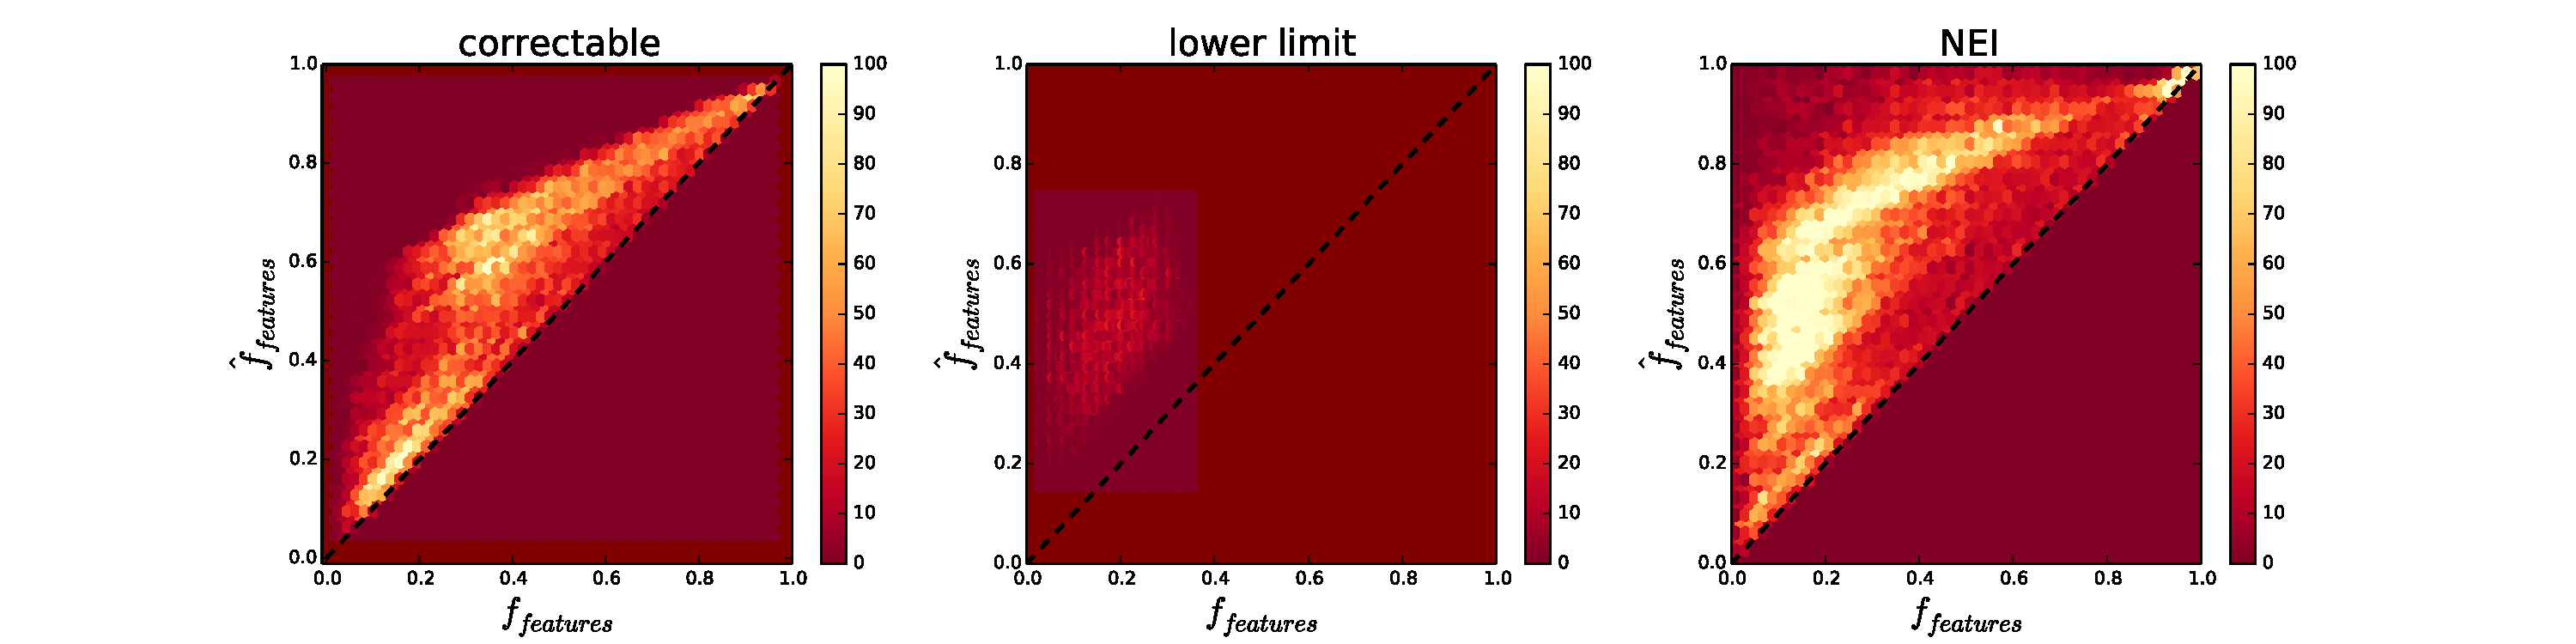
\includegraphics[width=\textwidth]{figures/debiased_corrections.pdf}
\caption{Debiased $p_{features}$ corrected to $z=0.3$ vs weighted $p_{features}$ for the correctable (left), uncorrectable (middle), and NEI (right) galaxies in the GZH sample.}

\label{fig:features_corrections}
\end{center}
\end{figure*}


%\subsection{Results of FERENGI analysis}
%
%{\bf Old text from Taiwan workshop}
%
%We show here the preliminary results of GZH classifications of images of galaxies placed at artificial redshifts. Figure~\ref{fig:ferengi_results_fake} shows the range of change of vote fractions for the change of $p_{\rm features}$ with redshift, for galaxies with different vote fraction levels, three ranges of surface-brightness levels and 7~evolutionary corrections (this last bit is indicated by the colour). 
%
%%-----------------------------------------------------------------------------------------------------------------------------------
%\begin{figure}
%\begin{center}
%
%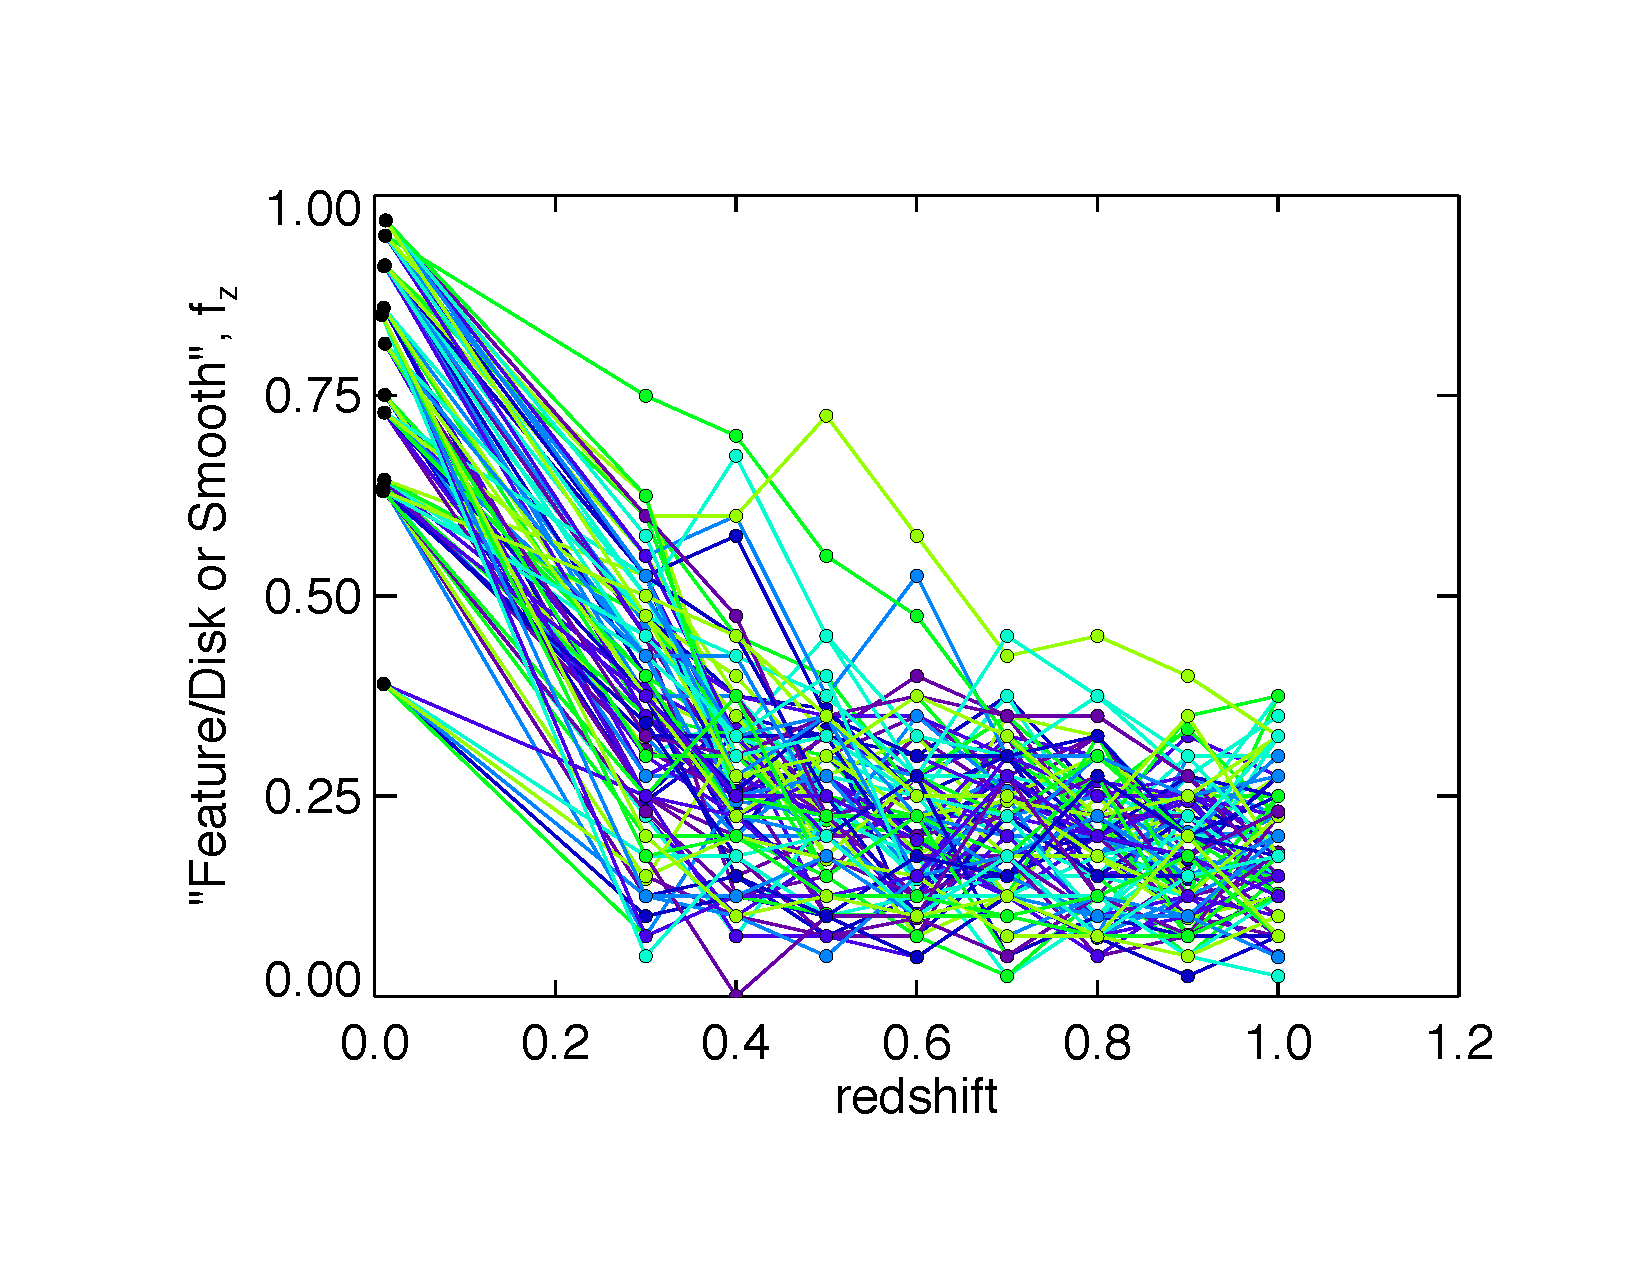
\includegraphics[width=0.45\textwidth]{figures/somewhat_fake_results.pdf}
%
%\caption{Preliminary results of the \ferengi{} redshifting exercise. WARNING NO USER WEIGHTING.... For a range of vote fraction levels with three surface-brightness levels and 7 evolutionary corrections each (the colours indicate evolutionary correction value with green being $e=0$, we show the range of evolution of the vote fractions for featured vs. smooth with redshift.}
%
%\label{fig:ferengi_results_fake}
%
%\end{center}
%\end{figure}
%%-----------------------------------------------------------------------------------------------------------------------------------


\subsubsection{TODO LIST}
We need to do: 
\begin{itemize}
\item Calculate the magnitudes, surface brightnesses and sizes of the galaxies in the FERENGI images....
\item Plot of magnitude distribution of galaxies in each of the four GZH subsamples with the magnitudes of our fake galaxies over plotted. 
\item Instructions of how to link the $z=0$ $p_X$ values for galaxies with a given size, magnitude (surface brightness) in the GZH images. 
\end{itemize}

\subsection{Morphological measurements in GZH beyond Task 1 - effects of debiasing?}
\subsection{Duplicate images}

\subsection{Effect of changing depth for GOODS}

\subsection{SDSS Stripe 82 images}

\subsection{Fake AGN}

\section{The Catalog}

The data release for GZH includes morphological data for 181,101 galaxies. The full table can be accessed at some website. We also include a secondary metadata table, which contains data from a variety of sources explained in Section \ref{sec:data}.

For each galaxy we list its unique objid, as well as the source's RA, DEC, and survey (AEGIS, COSMOS, GEMS, GOODS North (full and shallow depth), GOODS South (full and shallow depth), SDSS. For each of the 40 (?) questions in the GZH decision tree, the following classification data is provided: For each question, $\tt N_{votes}$ is the number of users to answer that question. For each unique answer, $\tt fraction$ is the fraction of users to select that answer ($\rm N_{answer}/N_{votes}$, and $\tt weighted$ is the weighted fraction, which takes into account user consistency (Section~\ref{sec:weighting}). 

The GZH vote fractions can be largely dependent on the resolution of the image. Two otherwise morphologically identical galaxies which differ significantly in redshift, brightness, or size may result in very different vote fractions for any given question, given that many features of a galaxy are difficult to discern in less-resolved images (bars, spiral arms, disk structure, etc). For this reason, it is necessary to take caution utilizing vote fractions as cut-offs to determine morphological structure; we offer guidelines for careful classification in Section~\ref{sec:cookbook}. 

We corrected for the biases described for the first question of the GZH decision tree, which asks ``Is the galaxy smooth and round, with no sign of a disk?'' The method is described in Section~\ref{sec:debiasing}. For this question, we provide the additional parameters $\tt debiased$, $\tt lower~limit$, $\tt upper~limit$, and $\tt best$ vote fractions. The $\tt best$ fraction for $p_{features}$is chosen based on the categorization of the galaxy: if it is ``correctable'', $\tt best = debiased$, if ``uncorrectable'', $\tt best = lower~limit$, and if neither, $\tt best = weighted$. The debiased vote fractions for $\tt p_{smooth}$ were calculated on the critera that vote fractions for all answers must sum to unity. Explicitely: $\tt p_{smooth} = 1 - p_{features} - p_{artifact}$. 

\tabletypesize{\scriptsize}
\begin{deluxetable}{lllllcrllllll|c}
\centering
\rotate
\tablecolumns{13}
\tablewidth{0pc}
\tablecaption{GZH morphological classifications for AEGIS, COSMOS, GEMS, and GOODS images} 
\label{tbl:catalog}
\tabletypesize{\scriptsize}
\tablehead{
 & & & RA & dec  &  
\multicolumn{2}{c}{\underline{t01\_smooth\_or\_features\_}} &
\multicolumn{6}{c}{\underline{t01\_smooth\_or\_features\_a01\_smooth\_}} &
\colhead{$\ldots$}
\\
\colhead{Project ID} & 
\colhead{Hubble ID} & 
\colhead{Imaging} & 
\colhead{J2000} & 
\colhead{J2000} & 
\colhead{Correction$^{1}$} & 
\colhead{$N_\mathrm{votes}$} & 
\colhead{fraction} & 
\colhead{weighted} & 
\colhead{debiased} & 
\colhead{best} &
\colhead{lower~limit} & 
\colhead{upper~limit} &
\colhead{}
}
\small
\startdata
AHZ100002g  & 10010842  & AEGIS             &          &            & 0        & 948       & 0.118    & 0.128     & 0.085    & 0.085    & 0.226     & 0.226    \\
AHZ100002h  & 10010870  & AEGIS             &          &            & 4        & 429       & 0.567    & 0.592     & 0.927    & 0.592    & $-$       & $-$      \\
$\ldots$    & $\ldots$  & $\ldots$          & $\ldots$ & $\ldots$   & $\ldots$ &  $\ldots$ & $\ldots$ & $\ldots$  & $\ldots$ & $\ldots$ & $\ldots$  & $\ldots$ \\
AHZ20004kd  & 20014731  & COSMOS            &          &            & 3        & 185       & 0.682    & 0.675     & 0.147    & 0.675    & $-$       & $-$      \\
AHZ20004ke  & 20014732  & COSMOS            &          &            & 2        & 149       & 0.689    & 0.756     & 0.893    & 0.756    & $-$       & $-$      \\
$\ldots$    & $\ldots$  & $\ldots$          & $\ldots$ & $\ldots$   & $\ldots$ &  $\ldots$ & $\ldots$ & $\ldots$  & $\ldots$ & $\ldots$ & $\ldots$  & $\ldots$ \\
AHZ400043g  & 90022729  & GEMS              &          &            & 1        & 400       & 0.702    & 0.733     & 0.487    & 0.734    & 0.483     & 0.800    \\
AHZ4000416  & 90022735  & GEMS              &          &            & 1        & 463       & 0.646    & 0.698     & 0.508    & 0.698    & 0.171     & 0.727    \\
$\ldots$    & $\ldots$  & $\ldots$          & $\ldots$ & $\ldots$   & $\ldots$ &  $\ldots$ & $\ldots$ & $\ldots$  & $\ldots$ & $\ldots$ & $\ldots$  & $\ldots$ \\
AGZ0007z47  & 10014     & GOODS-N-FULLDEPTH &          &            & 1        & 40        & 0.475    & 0.475     & 0.197    & 0.475    & 0.011     & 0.496    \\
AGZ0007z48  & 10017     & GOODS-N-FULLDEPTH &          &            & 3        & 40        & 0.675    & 0.675     & 0.048    & 0.675    & 0.168     & 0.669    \\
$\ldots$    & $\ldots$  & $\ldots$          & $\ldots$ & $\ldots$   & $\ldots$ &  $\ldots$ & $\ldots$ & $\ldots$  & $\ldots$ & $\ldots$ & $\ldots$  & $\ldots$ \\
AGZ00083jb  & 8869      & GOODS-S-FULLDEPTH &          &            & 1        & 40        & 0.425    & 0.425     & 0.109    & 0.425    & 0.070     & 0.548    \\
AGZ00083jc  & 8878      & GOODS-S-FULLDEPTH &          &            & 0        & 40        & 0.205    & 0.205     & 0.048    & 0.048    & $-$0.005  & 0.287    \\
\enddata
\tablenotetext{1}{Flag indicating how the vote fractions for this galaxy were corrected through debiasing (\S\ref{ssec:zeta_results}), if possible. 0~=~correctable, 1~=~uncorrectable ($p_{raw}$ --- $p_{adj}$ is not single-valued), 2~=~uncorrected ($z_{\rm gal} < 0.3$), 3~=~uncorrectable (insufficient FERENGI galaxies in this $z$-$\mu$ bin), 4~=~uncorrectable (no galaxy redshift available).}
\tablecomments{The full version of this table is available in electronic form, as well as at \url{http://data.galaxyzoo.org}. The complete version includes data for 118,425~galaxies and morphological information for all tasks in the tree. A subset of the information is shown here to illustrate form and content.}
\end{deluxetable}

% Why are some values negative?
% Why are most of the full-depth GOODS weighted fractions identical to the raw fractions?

\tabletypesize{\scriptsize}
\begin{deluxetable}{lllllcrllll|c}
\centering
\rotate
\tablecolumns{13}
\tablewidth{0pc}
\tablecaption{GZH morphological classifications for SDSS Stripe 82 single-epoch images} 
\label{tbl:stripe82_single}
\tabletypesize{\scriptsize}
\tablehead{
 & & & RA & dec  &  
\multicolumn{2}{c}{\underline{t01\_smooth\_or\_features\_}} &
\multicolumn{4}{c}{\underline{t01\_smooth\_or\_features\_a01\_smooth\_}} &
\colhead{$\ldots$}
\\
\colhead{Project ID} & 
\colhead{Hubble ID} & 
\colhead{Imaging} & 
\colhead{J2000} & 
\colhead{J2000} & 
\colhead{Correction$^{1}$} & 
\colhead{$N_\mathrm{votes}$} & 
\colhead{fraction} & 
\colhead{weighted} & 
\colhead{debiased} & 
\colhead{best} &
\colhead{}
}
\small
\startdata
AHZ5000001  &   587730845812064684  &   SDSS    &   &   &     2 &   41  &   0.585   &    0.595  &   0.759   &   0.594   \\
AHZ5000002  &   587730845812065247  &   SDSS    &   &   &     2 &   46  &   0.609   &    0.651  &   0.897   &   0.651   \\
AHZ5000003  &   587730845812196092  &   SDSS    &   &   &     2 &   51  &   0.039   &    0.044  &   0.067   &   0.043   \\
AHZ5000004  &   587730845812196825  &   SDSS    &   &   &     2 &   35  &   0.514   &    0.605  &   0.928   &   0.605   \\
AHZ5000005  &   587730845812524122  &   SDSS    &   &   &     2 &   47  &   0.766   &    0.812  &   1.038   &   0.810   \\
AHZ5000006  &   587730845812654984  &   SDSS    &   &   &     2 &   42  &   0.5	    &    0.542  &   0.680   &   0.541   \\
AHZ5000007  &   587730845812655541  &   SDSS    &   &   &     2 &   41  &   0.488   &    0.526  &   0.697   &   0.525   \\
AHZ5000008  &   587730845812720365  &   SDSS    &   &   &     2 &   53  &   0.792   &    0.84   &   1.050   &   0.839   \\
AHZ5000009  &   587730845812720640  &   SDSS    &   &   &     4 &   43  &   0.0	    &    0.0    &   0.0	    &   0.0	    \\
AHZ500000a  &   587730845812720699  &   SDSS    &   &   &     2 &   40  &   0.425   &    0.478  &   0.588   &   0.477   \\
$\ldots$    & $\ldots$  & $\ldots$  & $\ldots$  & $\ldots$   & $\ldots$ &  $\ldots$ & $\ldots$ & $\ldots$ \\
\enddata
\tablenotetext{1}{Flag indicating how the vote fractions for this galaxy were corrected through debiasing (\S\ref{ssec:zeta_results}), if possible. 0~=~correctable, 1~=~uncorrectable ($p_{raw}$ --- $p_{adj}$ is not single-valued), 2~=~uncorrected ($z_{\rm gal} < 0.3$), 3~=~uncorrectable (insufficient FERENGI galaxies in this $z$-$\mu$ bin), 4~=~uncorrectable (no galaxy redshift available).}
\tablecomments{The full version of this table is available in electronic form, as well as at \url{http://data.galaxyzoo.org}. The complete version includes data for 21,522~galaxies and morphological information for all tasks in the tree. A subset of the information is shown here to illustrate form and content.}
\end{deluxetable}



\tabletypesize{\scriptsize}
\begin{deluxetable}{lllllcrllll|c}
\centering
\rotate
\tablecolumns{13}
\tablewidth{0pc}
\tablecaption{GZH morphological classifications for SDSS Stripe 82 coadded images} 
\label{tbl:stripe82_coadd}
\tabletypesize{\scriptsize}
\tablehead{
 & & & RA & dec  &  
\multicolumn{2}{c}{\underline{t01\_smooth\_or\_features\_}} &
\multicolumn{4}{c}{\underline{t01\_smooth\_or\_features\_a01\_smooth\_}} &
\colhead{$\ldots$}
\\
\colhead{Project ID} & 
\colhead{Hubble ID} & 
\colhead{Imaging} & 
\colhead{J2000} & 
\colhead{J2000} & 
\colhead{Correction$^{1}$} & 
\colhead{$N_\mathrm{votes}$} & 
\colhead{fraction} & 
\colhead{weighted} & 
\colhead{debiased} & 
\colhead{best} &
\colhead{}
}
\small
\startdata
AHZ6000001  & 8647474690312306978   &   SDSS    &   &   &    4  & 40  & 0.275   &    0.289  &   0.762   &   0.289   & \\
AHZ6000002  & 8647474690312307154   &   SDSS    &   &   &    2  & 43  & 0.605   &    0.634  &   0.858   &   0.635   & \\
AHZ6000003  & 8647474690312307877   &   SDSS    &   &   &    2  & 51  & 0.608   &    0.627  &   0.906   &   0.627   & \\
AHZ6000004  & 8647474690312308301   &   SDSS    &   &   &    4  & 52  & 0.038   &    0.038  &   0.723   &   0.038   & \\
AHZ6000005  & 8647474690312308318   &   SDSS    &   &   &    2  & 44  & 0.614   &    0.632  &   0.776   &   0.631   & \\
AHZ6000006  & 8647474690312308880   &   SDSS    &   &   &    2  & 36  & 0.667   &    0.683  &   0.901   &   0.683   & \\
AHZ6000007  & 8647474690312372644   &   SDSS    &   &   &    4  & 48  & 0.646   &    0.674  &   1.145   &   0.674   & \\
AHZ6000008  & 8647474690312372789   &   SDSS    &   &   &    4  & 45  & 0.489   &    0.571  &   0.964   &   0.570   & \\
AHZ6000009  & 8647474690312372931   &   SDSS    &   &   &    4  & 47  & 0.553   &    0.587  &   0.926   &   0.587   & \\
AHZ600000a  & 8647474690312373190   &   SDSS    &   &   &    4  & 47  & 0.574   &    0.559  &   1.008   &   0.559   & \\
$\ldots$    & $\ldots$  & $\ldots$  & $\ldots$  & $\ldots$   & $\ldots$ &  $\ldots$ & $\ldots$ & $\ldots$ \\
\enddata
\tablenotetext{1}{Flag indicating how the vote fractions for this galaxy were corrected through debiasing (\S\ref{ssec:zeta_results}), if possible. 0~=~correctable, 1~=~uncorrectable ($p_{raw}$ --- $p_{adj}$ is not single-valued), 2~=~uncorrected ($z_{\rm gal} < 0.3$), 3~=~uncorrectable (insufficient FERENGI galaxies in this $z$-$\mu$ bin), 4~=~uncorrectable (no galaxy redshift available).}
\tablecomments{The full version of this table is available in electronic form, as well as at \url{http://data.galaxyzoo.org}. The complete version includes data for 30,339~galaxies and morphological information for all tasks in the tree. A subset of the information is shown here to illustrate form and content.}
\end{deluxetable}

To include: detailed description of each column in the machine-readable tables. 

Needs some test cases for extracting a given set of objects (eg, clump galaxies in a particular redshift range) and evaluation of the results. Possibly include suggested thresholds, \'a la GZ2. 
\section{Using the catalog}
\label{sec:cookbook}
Include cookbook for selecting morphologies. 
\section{Analysis}

\subsection{Demographics of morphology}

Summarize the broad trends that are seen regarding the fraction of galaxies with various morphologies, how that relates to color, size, etc. Briefly discuss results as compared with literature and theory. 

\subsection{Comparison to other catalogs}

Compare GZH data to:

\begin{itemize}
    \item \citet[ZEST;][]{sca07} (COSMOS)
    \item Tasca (COSMOS)
    \item Cassata (COSMOS)
    \item Zajmoski (COSMOS)
    \item GEMS morphologies?
    \item AEGIS morphologies?
    \item GOODS N/S morphologies?
    \item expert visual inspection?
\end{itemize}

\textit{Address trends seen in broad morphological classes, possible reasons for difference. Also should attempt to map between the GZH vote fractions and whatever classification systems are used in the above systems.}

\section{Summary}

Now people go and do science with these awesome GZH classifications.  
 
\paragraph*{ACKNOWLEDGEMENTS.} 

This publication has been made possible by the participation of more than 200,000 volunteers in the Galaxy Zoo project. Their contributions are individually acknowledged at \texttt{http://www.galaxyzoo.org/volunteers}.

We thank Meg Schwamb and the ASIAA for hosting the ``Citizen Science in Astronomy'' workshop, 3-7 Mar 2014 in Taipei, Taiwan, at which some of this analysis was done. 

This project made heavy use of the Astropy packages in Python \citep{ast13}, the \texttt{seaborn} plotting package \citep{was15}, and astroML \citep{van12}.

HST acknowledgements.

Funding for the SDSS and SDSS-II has been provided by the Alfred P. Sloan Foundation, the Participating Institutions, the National Science Foundation, the U.S. Department of Energy, the National Aeronautics and Space Administration, the Japanese Monbukagakusho, the Max Planck Society, and the Higher Education Funding Council for England. The SDSS website is http://www.sdss.org/. 

The SDSS is managed by the Astrophysical Research Consortium for the Participating Institutions. The Participating Institutions are the American Museum of Natural History, Astrophysical  Institute Potsdam, University of Basel, University of Cambridge, Case Western Reserve University, University of Chicago, Drexel University, Fermilab, the Institute for Advanced Study, the Japan Participation Group, Johns Hopkins University, the Joint Institute for Nuclear Astrophysics, the Kavli Institute for Particle Astrophysics and Cosmology, the Korean Scientist Group, the Chinese Academy of Sciences (LAMOST), Los Alamos National Laboratory, the Max-Planck-Institute for Astronomy (MPIA), the Max-Planck-Institute for Astrophysics (MPA), New Mexico State University, Ohio State University, University of Pittsburgh, University of Portsmouth, Princeton University, the United States Naval Observatory and the University of Washington. 

\bibliography{kwrefs}

\newpage
\clearpage
\appendix
\section{GOODS Shallow Depth data}


\begin{table}
\caption{Breakdown of what we can correct out of the GOODS shallow depth data. \label{goods_shallow_categories}}
\begin{tabular}{lrrrrrrrr}
\hline\hline
                                   & GOODS-N & GOODS-S & Total \\
\hline
Correctable                        & 748     & 514     & 1,262 \\
Uncorrectable                      & 526     & 1,143   & 1,669 \\
No Correction Needed ($z \le 0.3$) & 267     & 267     & 534   \\ 
NEI                                & 851     & 2,670   & 3,521 \\
No Redshift Information            & 159     & 319     & 478   \\
Total                              & 2,551   & 4,913   & 7,464 \\
\hline\hline
\end{tabular}
\end{table}



GZH used both 5-epoch and 2-epoch sets of data to construct the GOODS set of images. The 11,157 full depth 5-epoch images are used in the main catalog; the classifications for the 7,464 shallow depth 2-epoch images are offered as a supplementary table. Here we briefly analyze the effect of image depth on the ability of the GZ users to identify features or disk structure in the images. 

\subsection{Comparing shallow and full depth morphologies}.
Of the 11,157 galaxies in the GOODS-N and GOODS-S full depth sample, 4,461 of these are in the shallow-depth sample. In Figure~\ref{fig:shallow_vs_full} we find a strong correlation between $\rm p_{features}$ for both sets of images. The mean change in $\rm p_{features}$ from the shallow to full depth images  $\rm p_{features,full} - p_{features,shallow} = \Delta p = 0.00$, with a standard deviation of $\sigma = 0.17$. While there is some variance in $\Delta p$ in the whole sample, the change is usually small and not often significant enough to change a morphological classification. Defining a clean sample of disk galaxies as those with $p_{features,best}>0.8$, elliptical galaxies as those with  $p_{smooth,best}<0.2$, and intermediate as those in between, we find that 75\% of the sample would not change morphology. Of the remaining 25\% that would change morphology, only 0.3\% (representing 10 galaxies total) drastically change morphology from smooth to featured or visa versa, while the rest would transition to or from the ``intermediate'' morphology. Details can be seen in Table~\ref{shallow_to_full_stats} and examples of images representing the 9 possible changes (or lack of) in morphology are shown in Figures~\ref{fig:shallow_smooth},\ref{fig:shallow_intermediate}, and \ref{fig:shallow_featured}.

\begin{figure}
\begin{center}
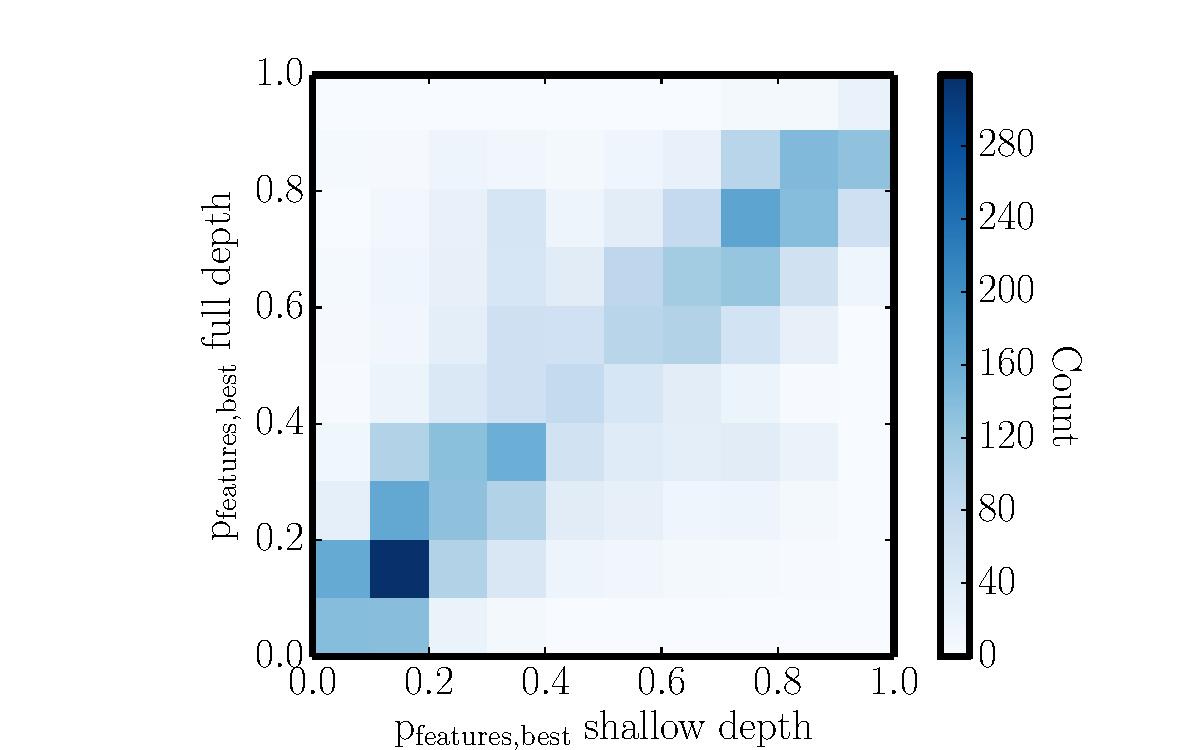
\includegraphics[width=0.50\textwidth]{figures/full_shallow_p_plot.pdf}
\caption{shallowfull}
\label{fig:shallow_vs_full}
\end{center}
\end{figure}

\begin{table}
\caption{Properties of galaxies whose morphologies changed or stayed the same in the shallow vs full images. Featured here is defined as $p_{features,best}>0.8$, intermediate = $0.2<p_{features,best}<0.8$, smooth = $p_{smooth,best}<0.2$. \label{shallow_to_full_stats}}
\begin{tabular}{lrrrrrrrr}
\hline\hline
shallow to full morphology    & N       & \%       & $<\Delta p>$ & $<z>$ \\
\hline
smooth to smooth              & 758     & 17.0     & -0.00        &  0.69\\
smooth to intermediate        & 367     & 8.2      & 0.18         &  0.69\\
smooth to featured            & 7       & 0.2      & 0.76         &  0.57\\ 
intermediate to smooth        & 214     & 4.8      & -0.18        &  0.65\\
intermediate to intermediate  & 2,303   & 51.6     & 0.01         &  0.78 \\
intermediate to featured      & 168     & 3.8      & 0.19         &  0.83\\
featured to smooth            & 3       & 0.1      & -0.74        &  0.71\\
featured to intermediate      & 337     & 7.6      & -0.18        &  0.68\\
featured to featured          & 301     & 6.8      & -0.05        &  0.71\\

Total                         & 4,461   & 100      &              & \\
\hline\hline
\end{tabular}
\end{table}



\begin{figure*}
\centering

\subfigure{[a]\label{fig:smoothtoint}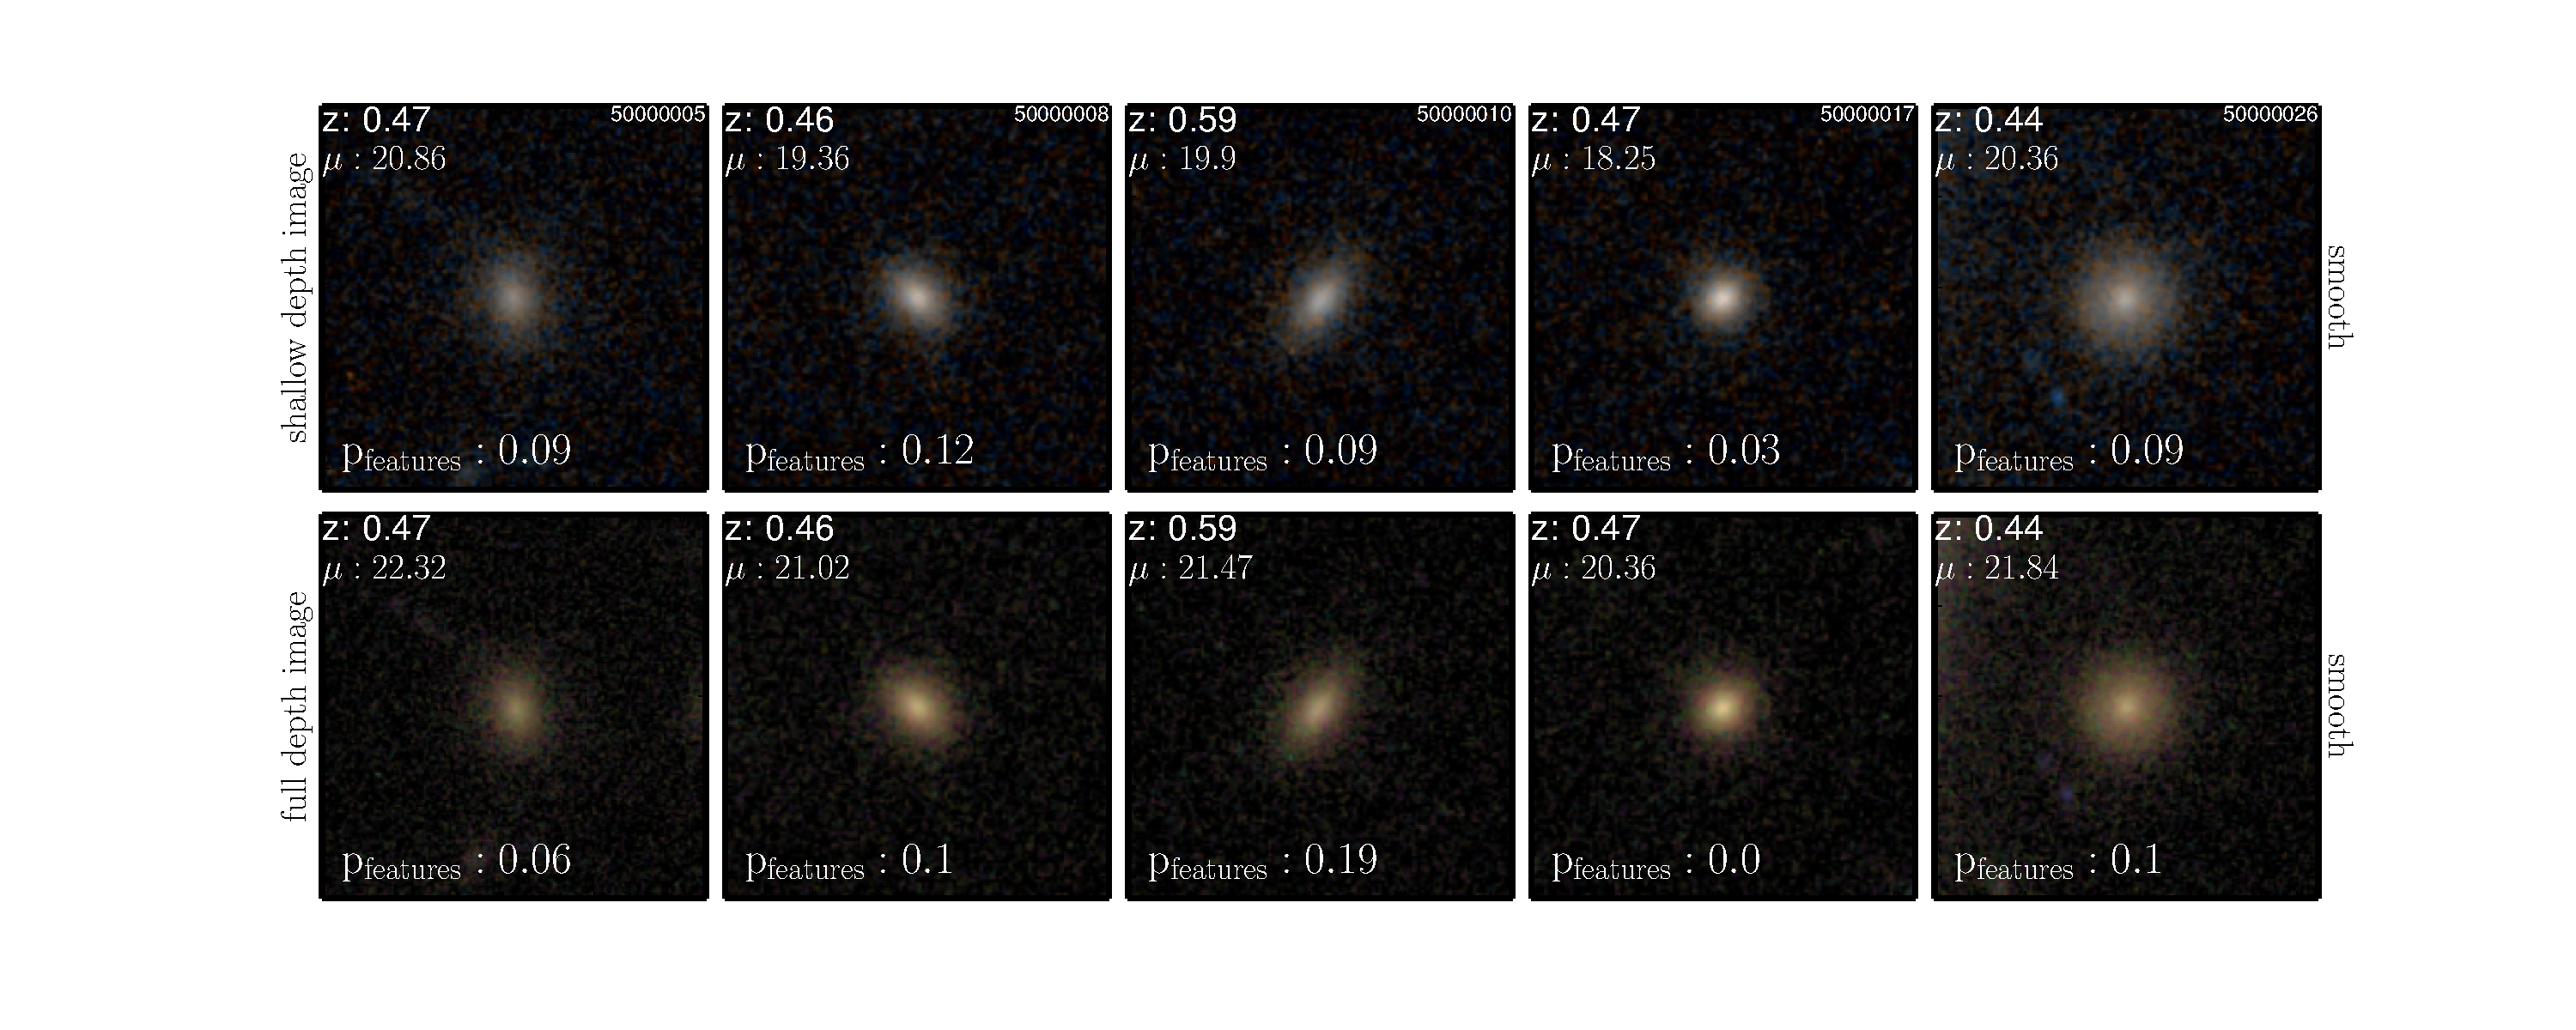
\includegraphics[width=\textwidth]{figures/smooth_to_smooth.pdf}}

\subfigure{[b]\label{fig:smoothtoint}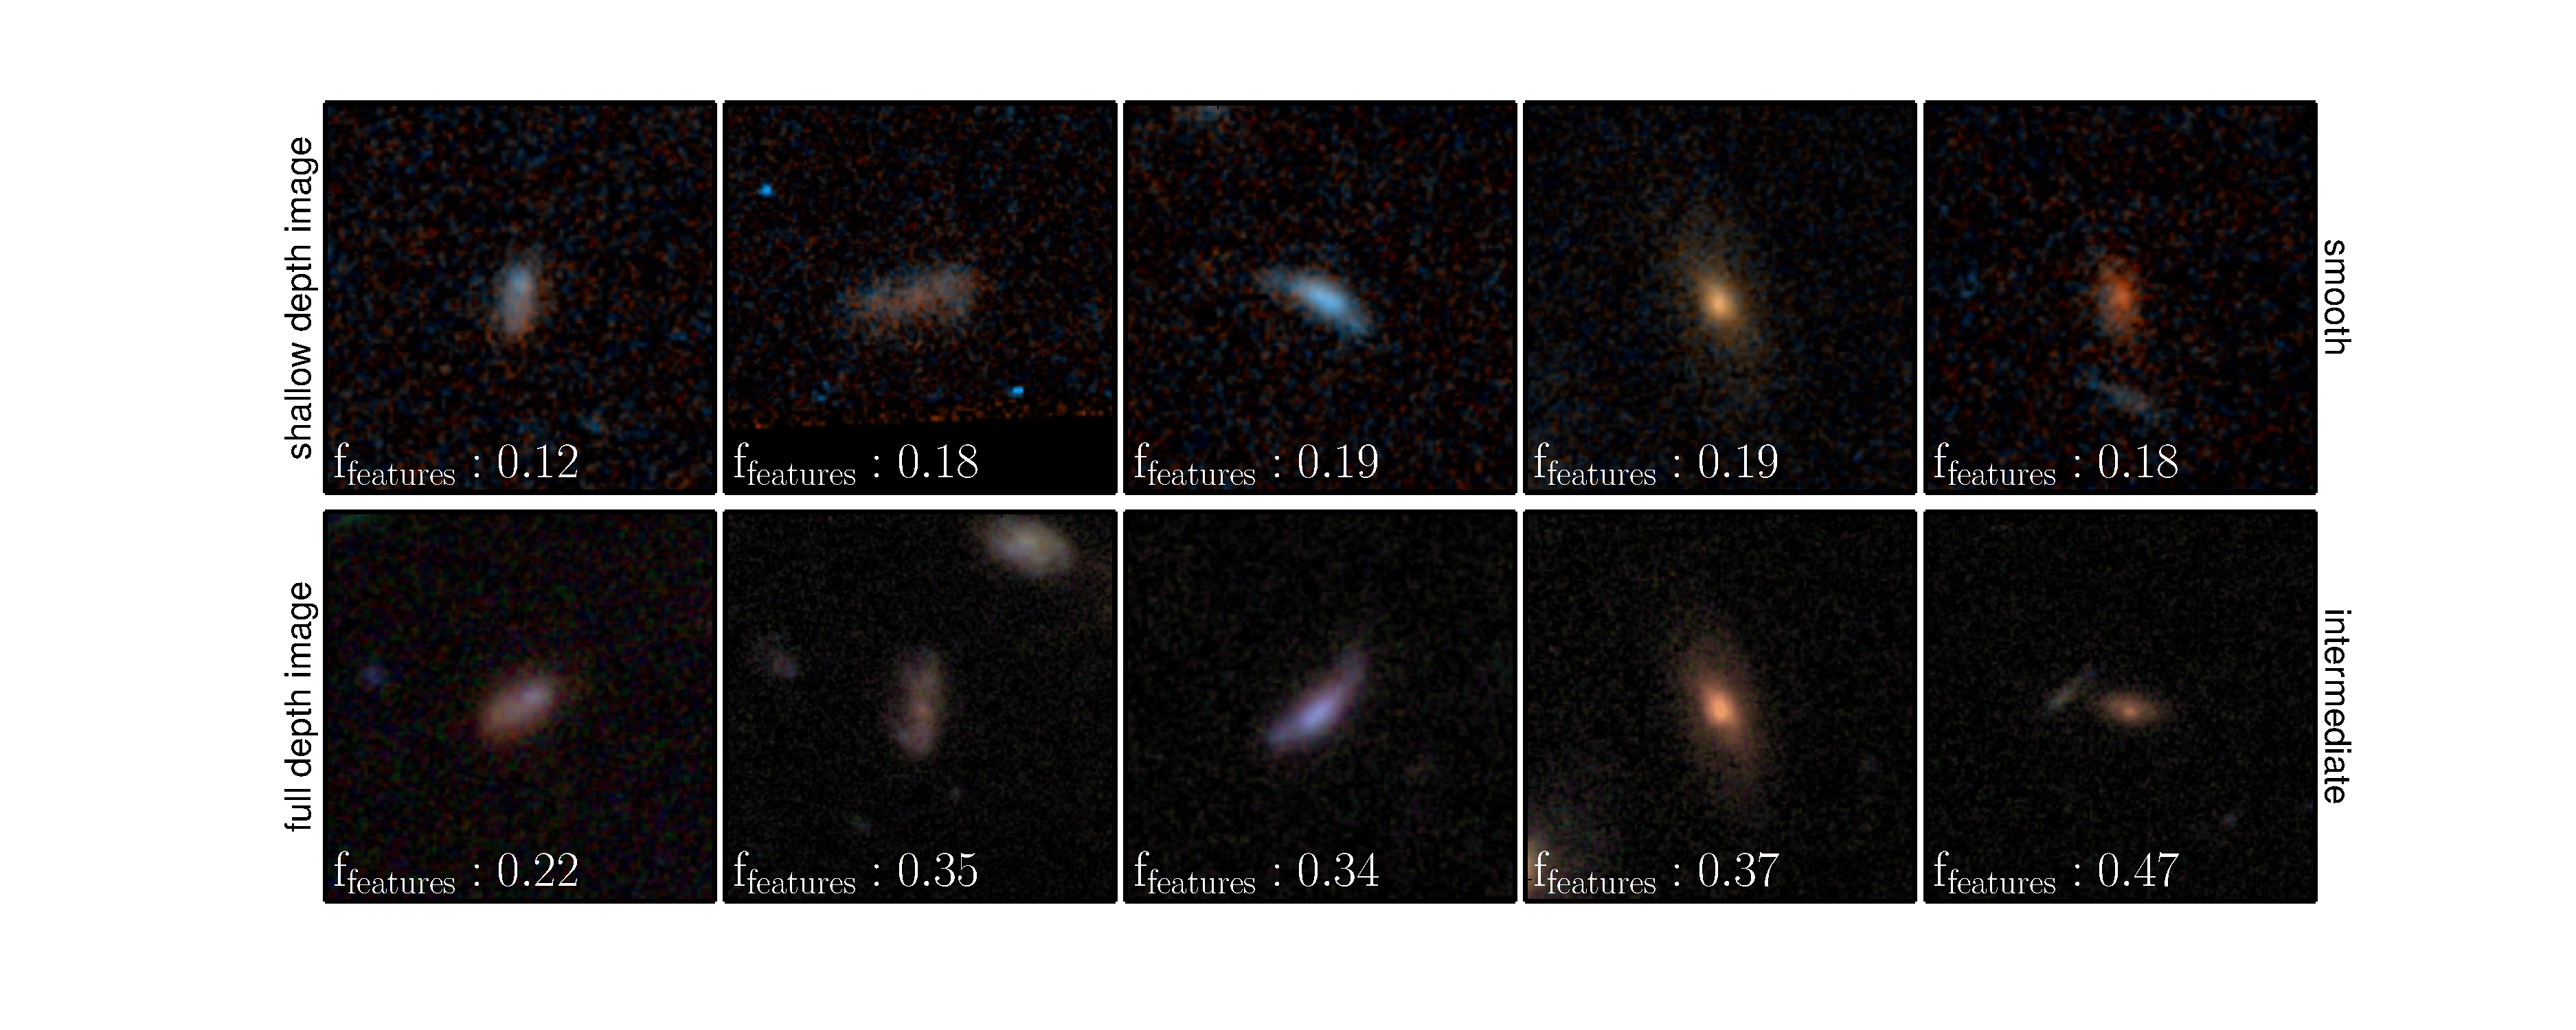
\includegraphics[width=\textwidth]{figures/smooth_to_intermediate.pdf}}

\subfigure{[c]\label{fig:smoothtoint}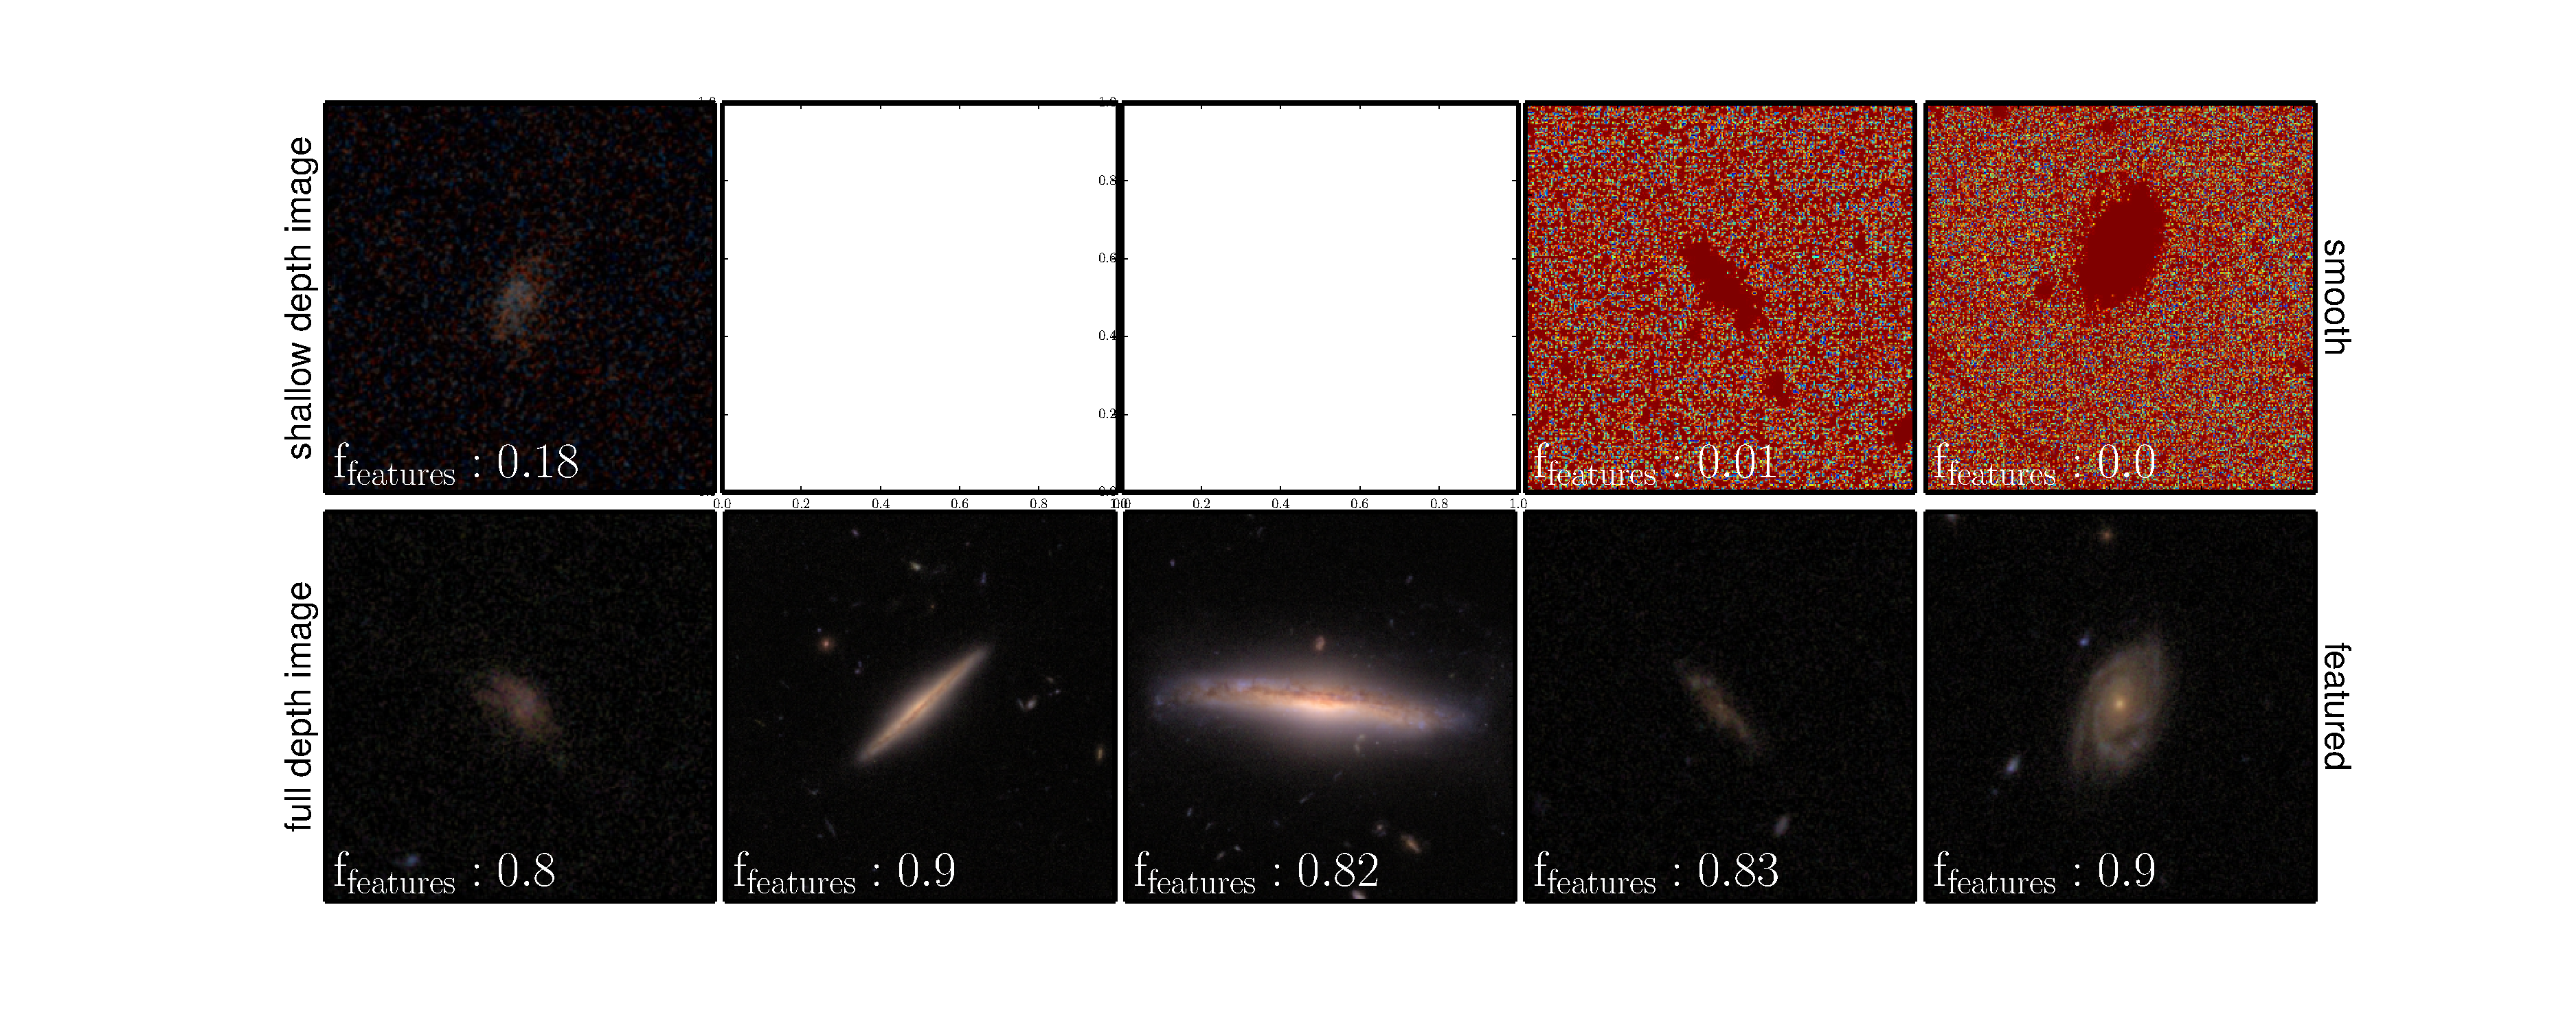
\includegraphics[width=\textwidth]{figures/smooth_to_featured.pdf}}

\caption{Galaxies whose shallow images were classified as smooth and full depth images were classified as smooth, intermediate, or featured.}
\label{fig:shallow_smooth}
\end{figure*}

\begin{figure*}
\centering

\subfigure{[b]\label{fig:smoothtoint}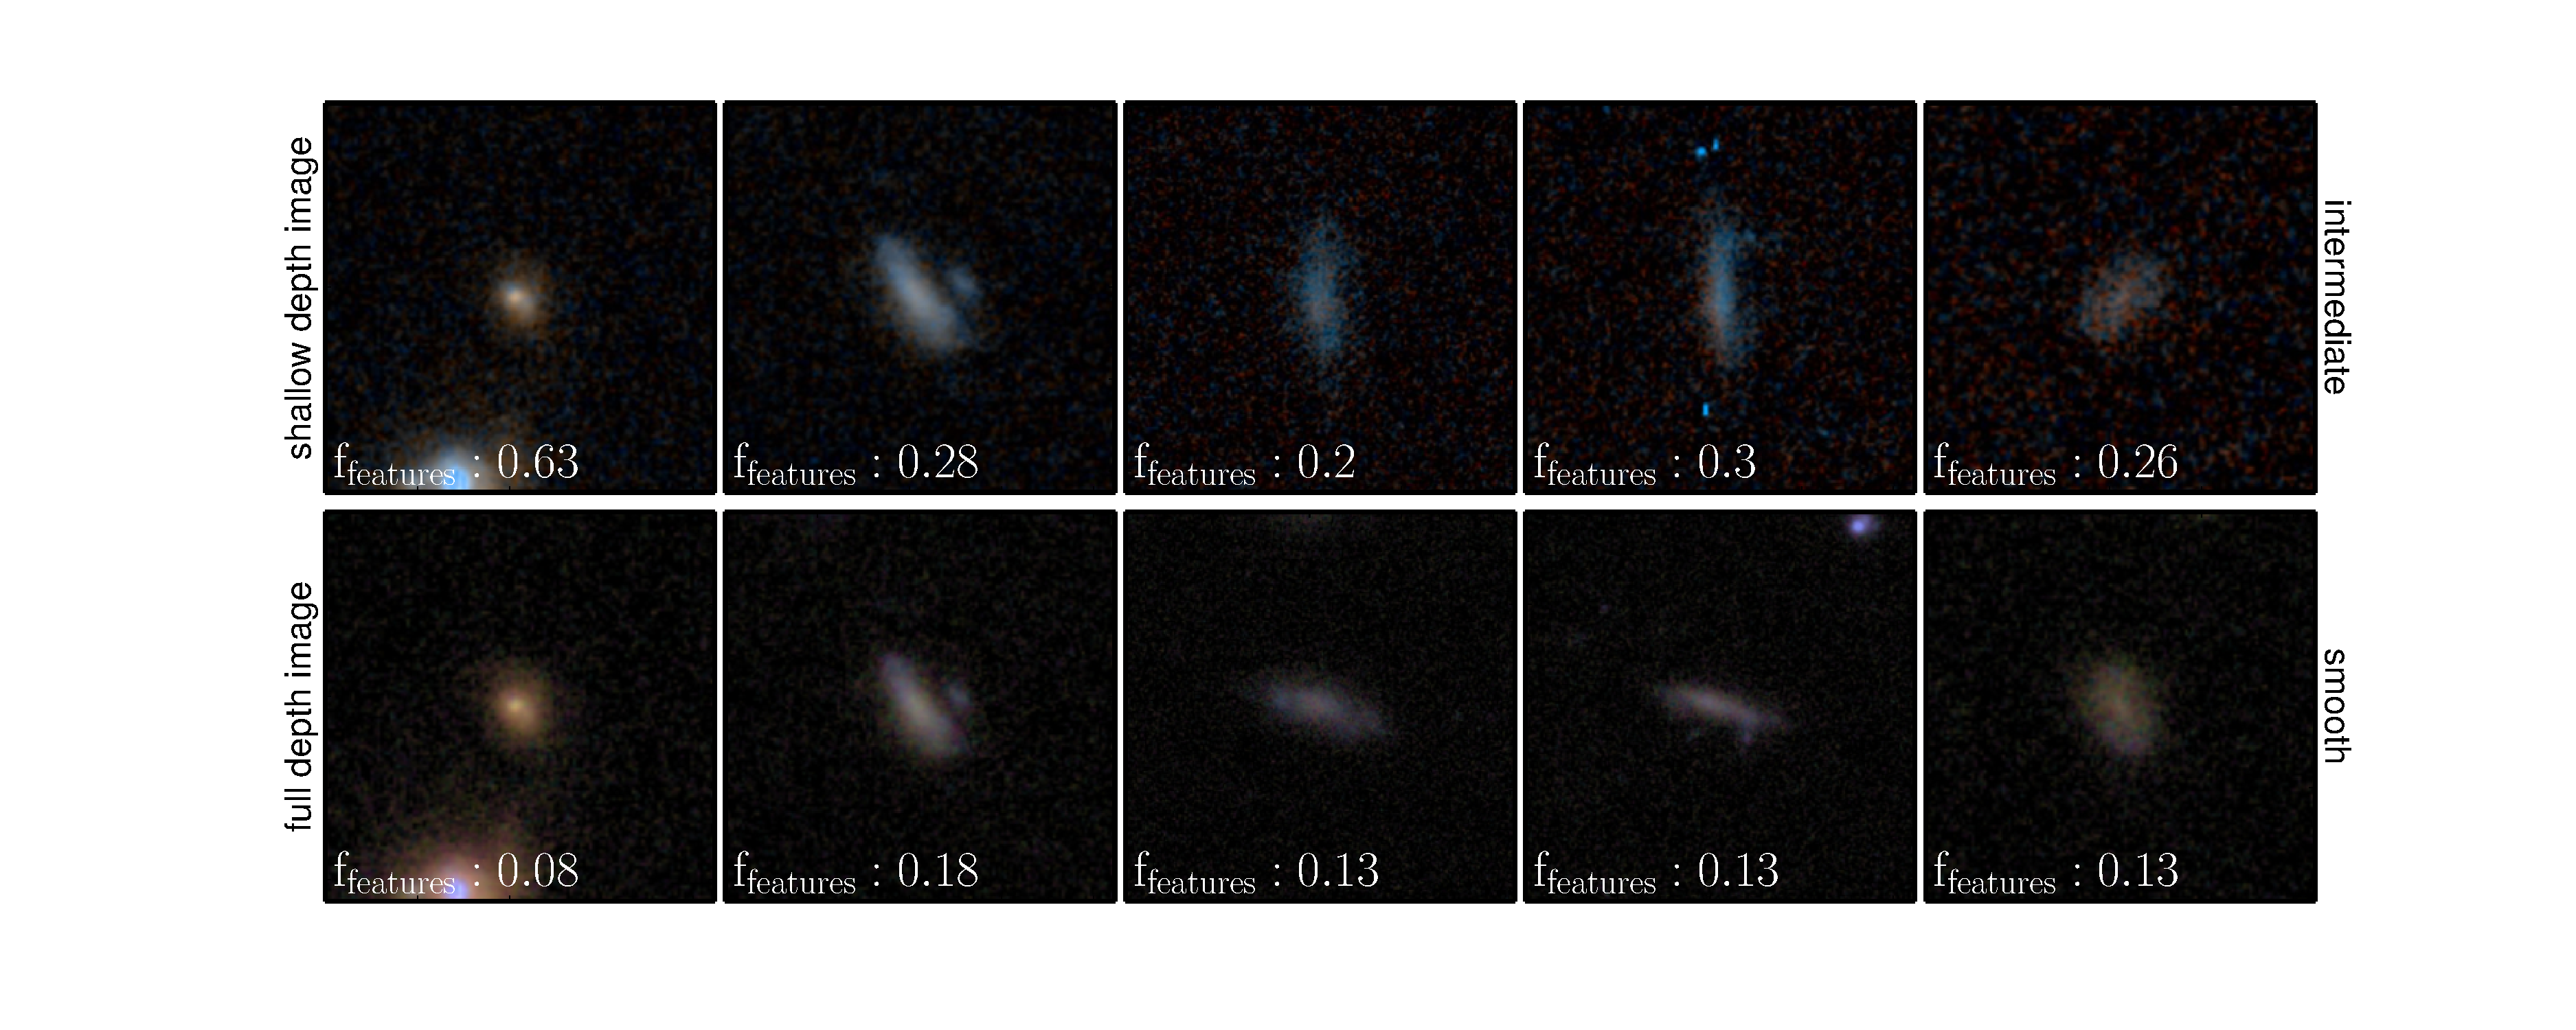
\includegraphics[width=\textwidth]{figures/intermediate_to_smooth.pdf}}

\subfigure{[b]\label{fig:smoothtoint}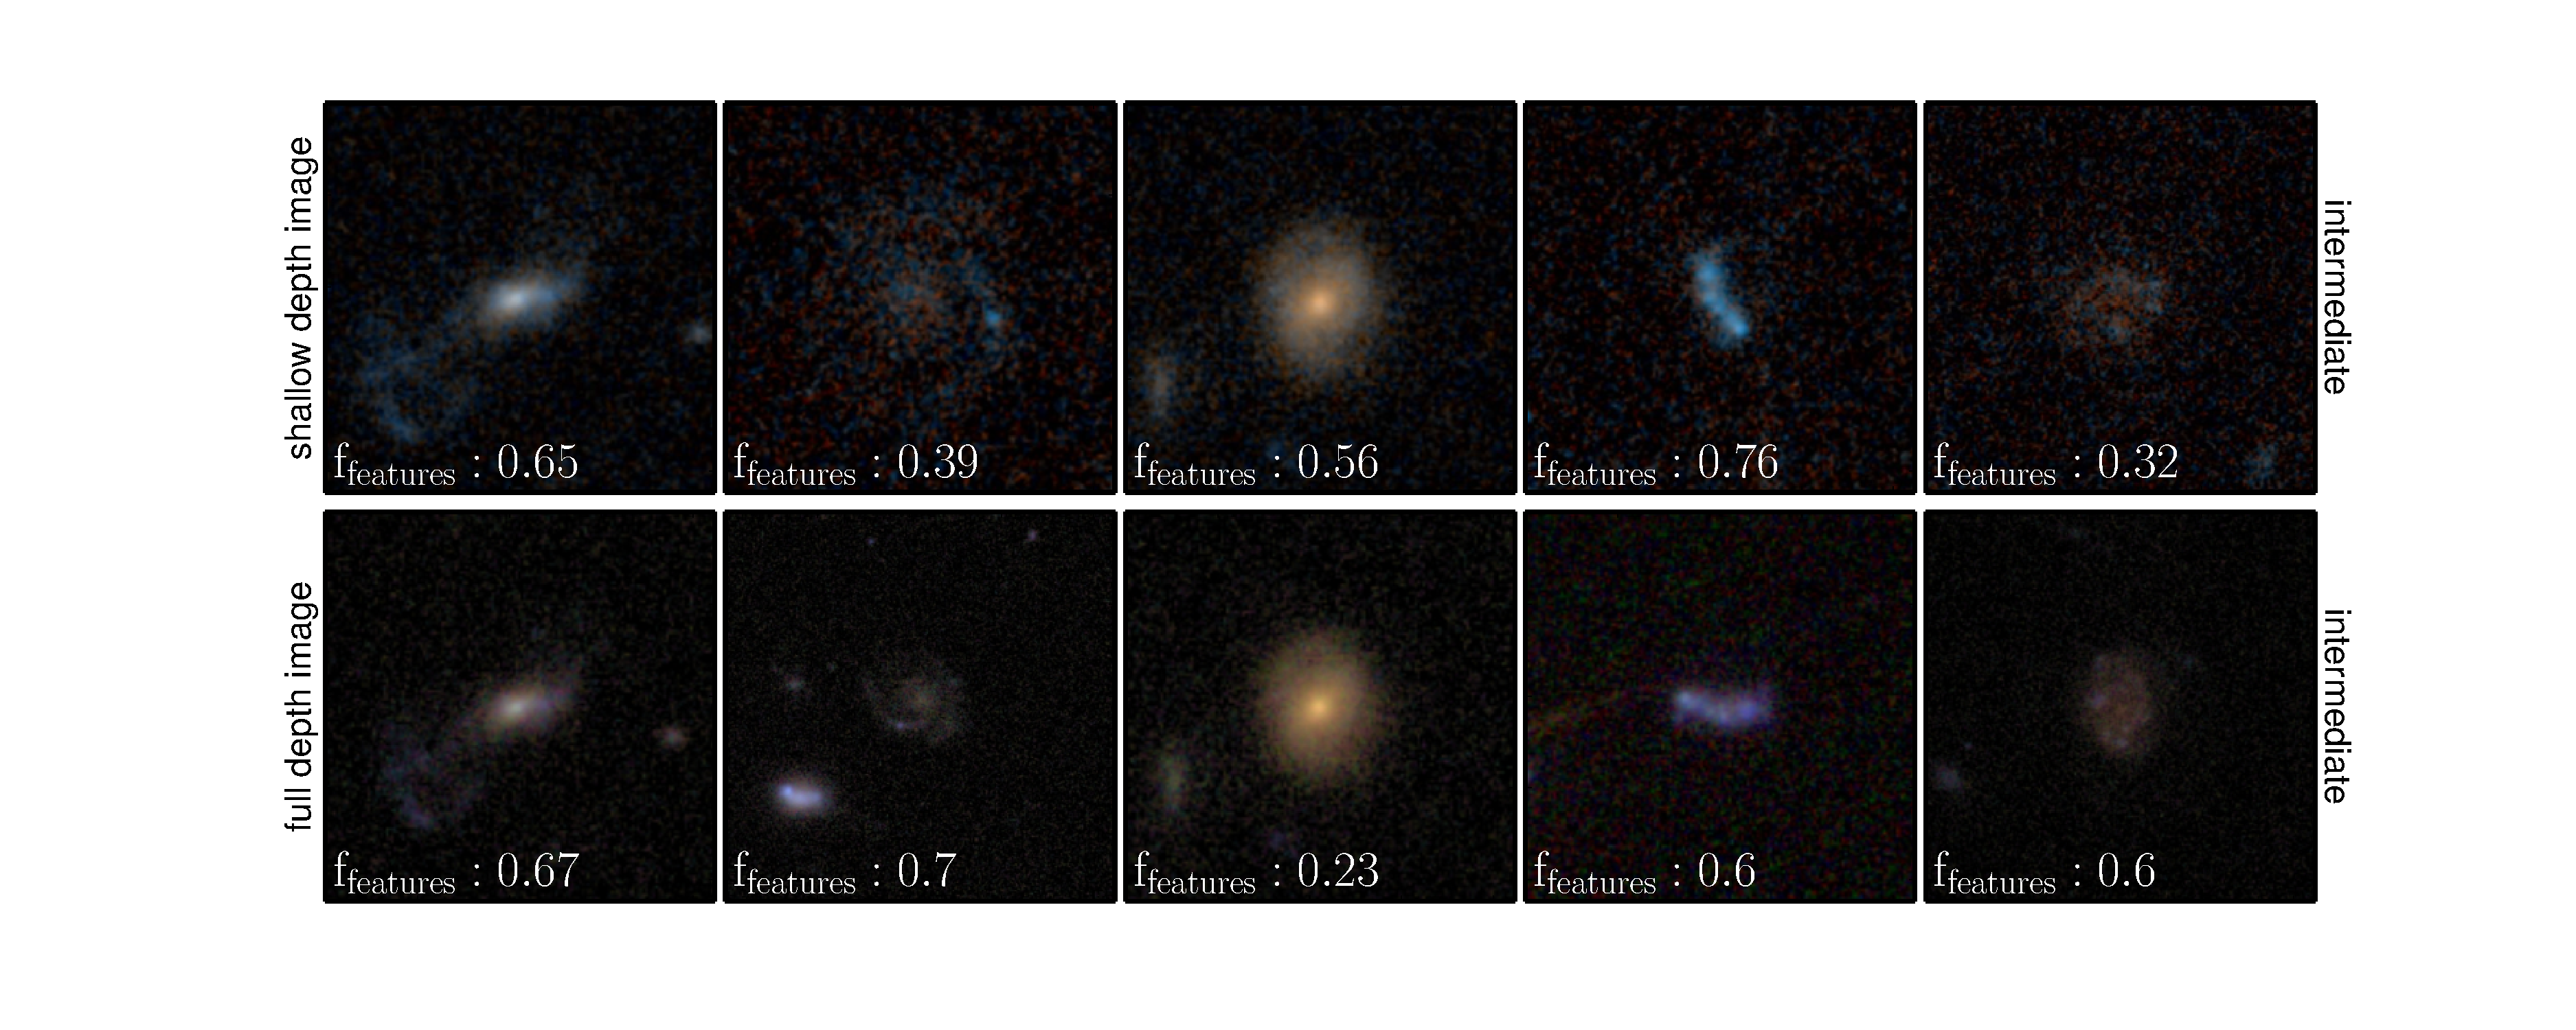
\includegraphics[width=\textwidth]{figures/intermediate_to_intermediate.pdf}}

\subfigure{[b]\label{fig:smoothtoint}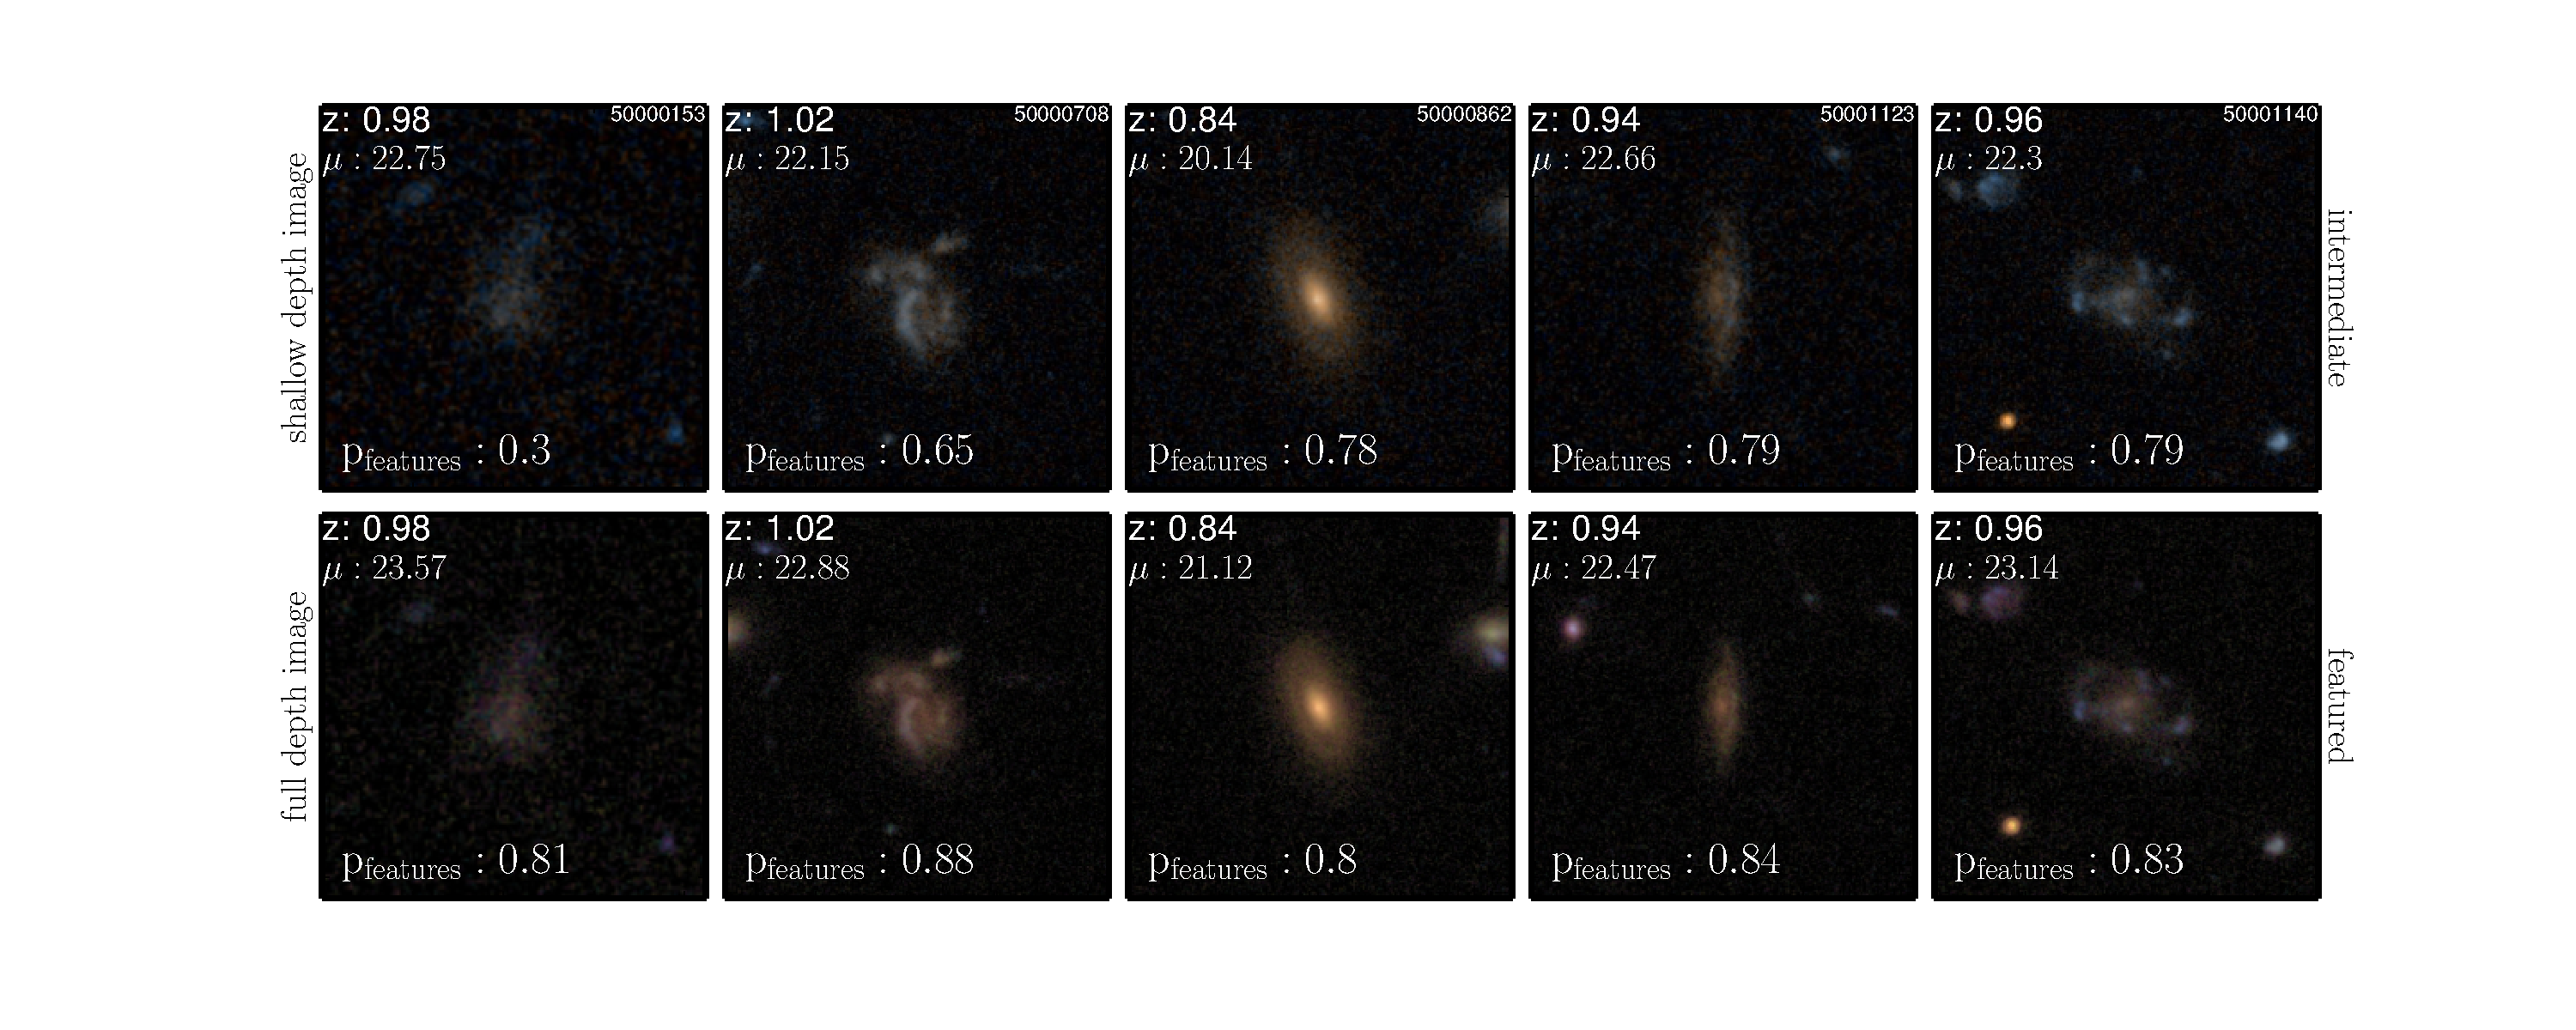
\includegraphics[width=\textwidth]{figures/intermediate_to_featured.pdf}}

\caption{Galaxies whose shallow images were classified as intermediate and full depth images were classified as smooth, intermediate, or featured.}
\label{fig:shallow_intermediate}
\end{figure*}

\begin{figure*}
\centering

\subfigure{[b]\label{fig:smoothtoint}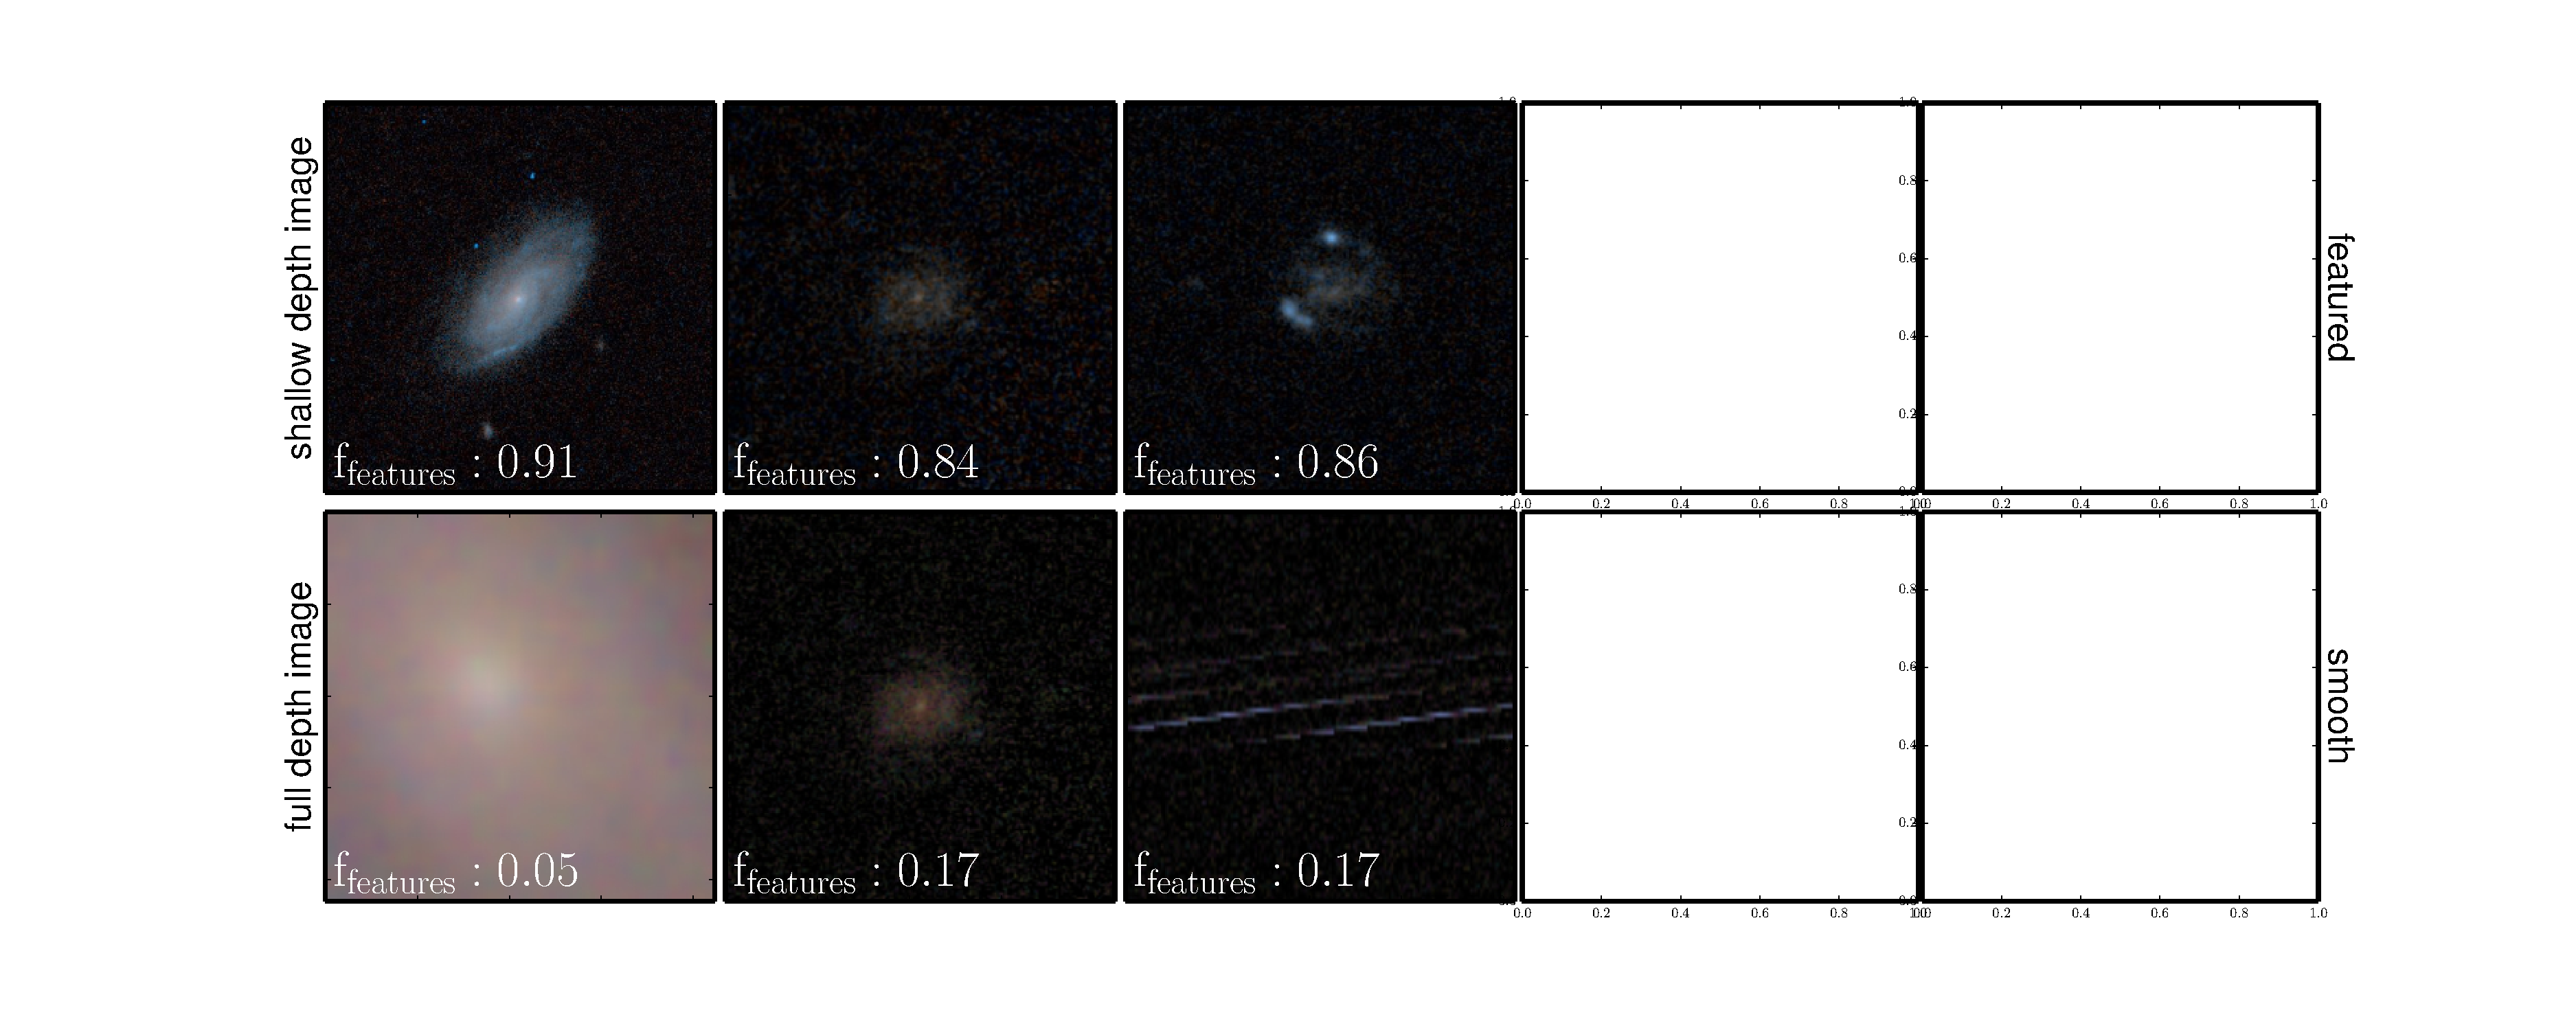
\includegraphics[width=\textwidth]{figures/featured_to_smooth.pdf}}

\subfigure{[b]\label{fig:smoothtoint}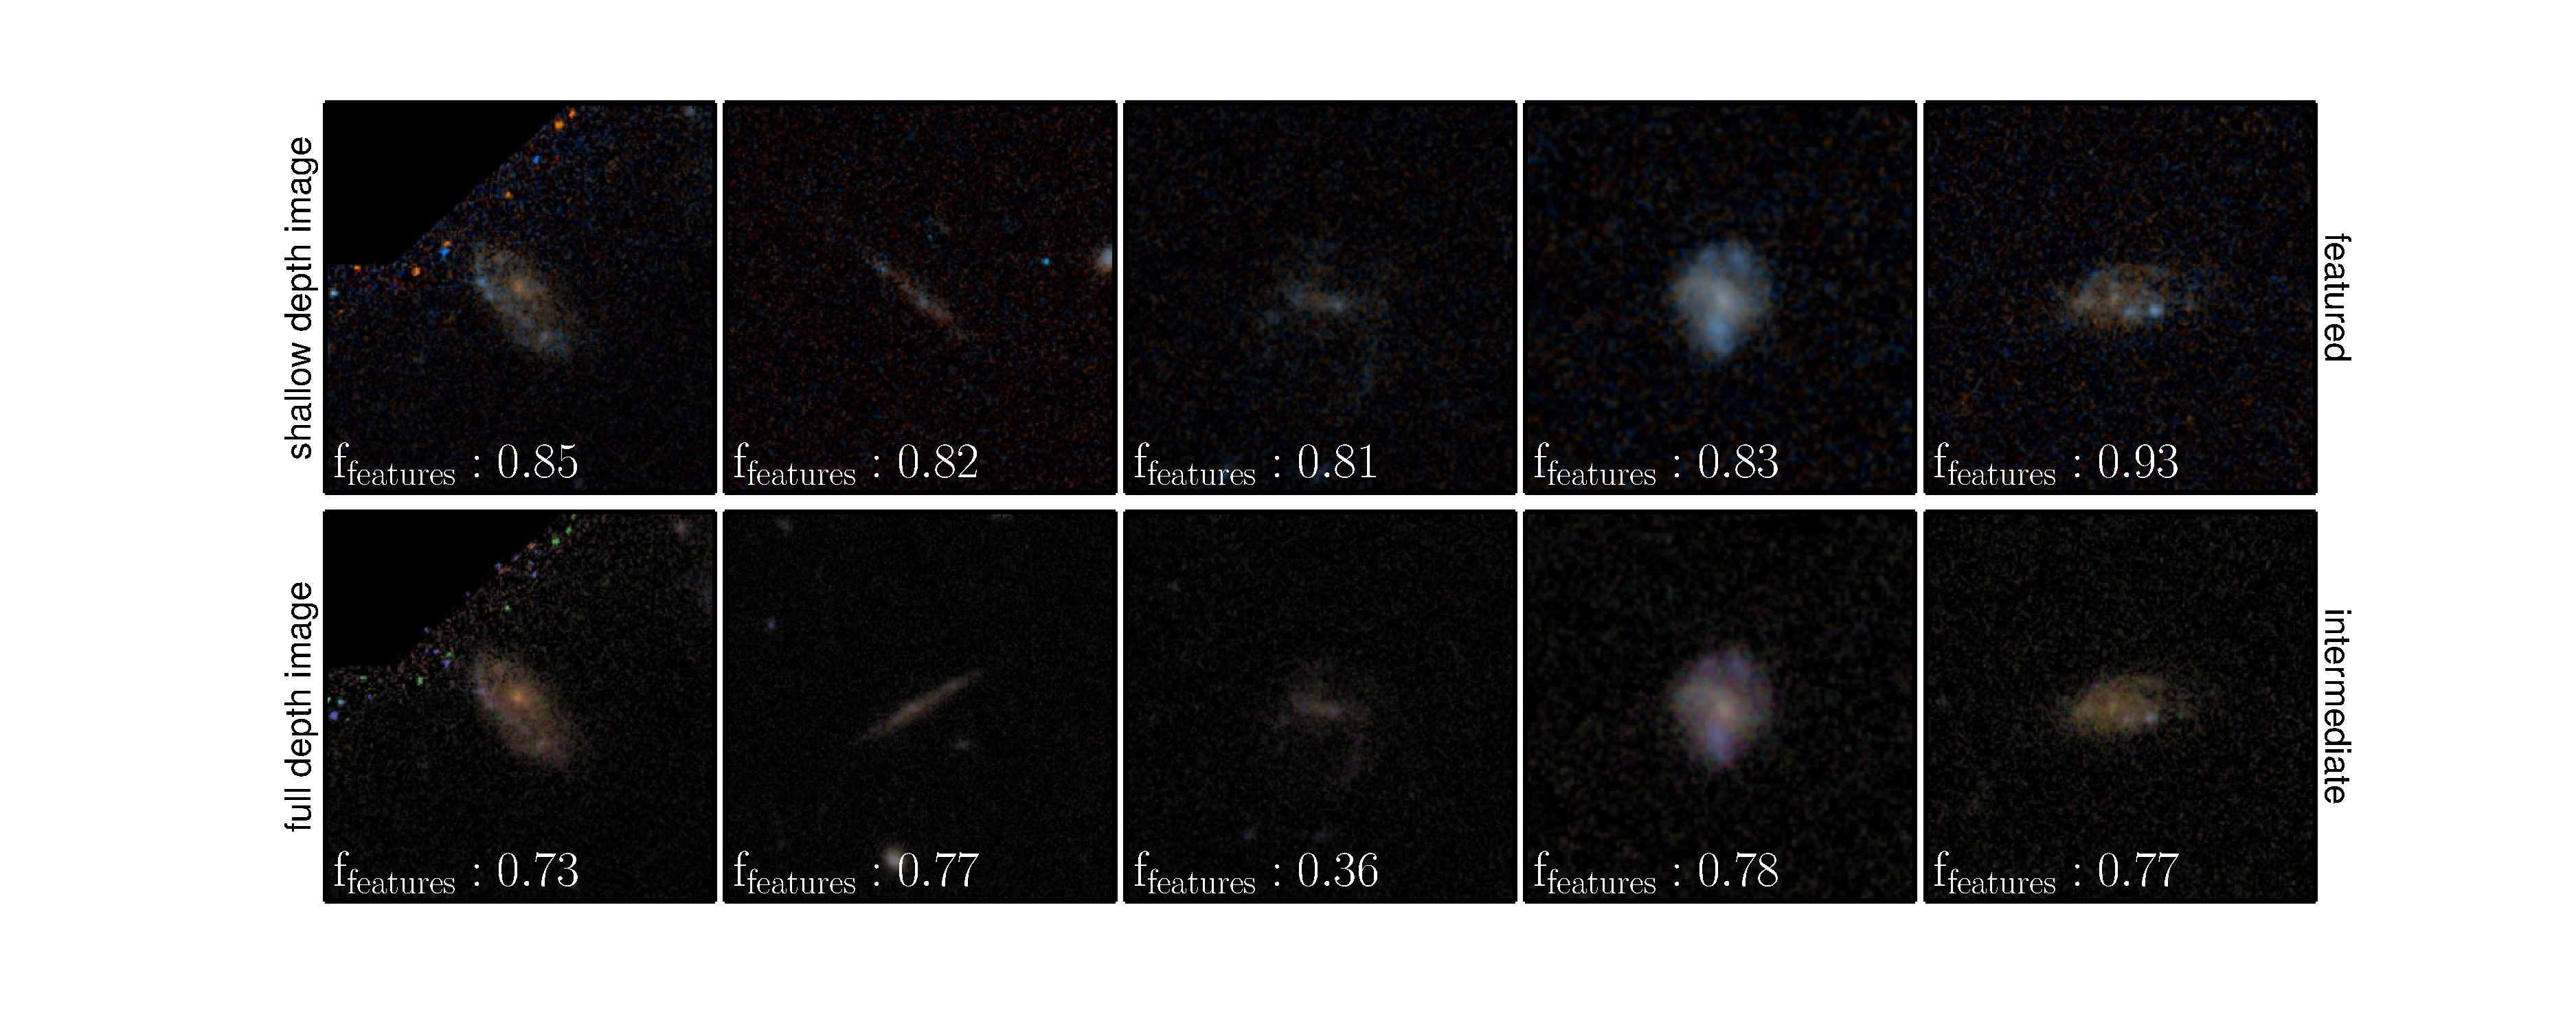
\includegraphics[width=\textwidth]{figures/featured_to_intermediate.pdf}}

\subfigure{[b]\label{fig:smoothtoint}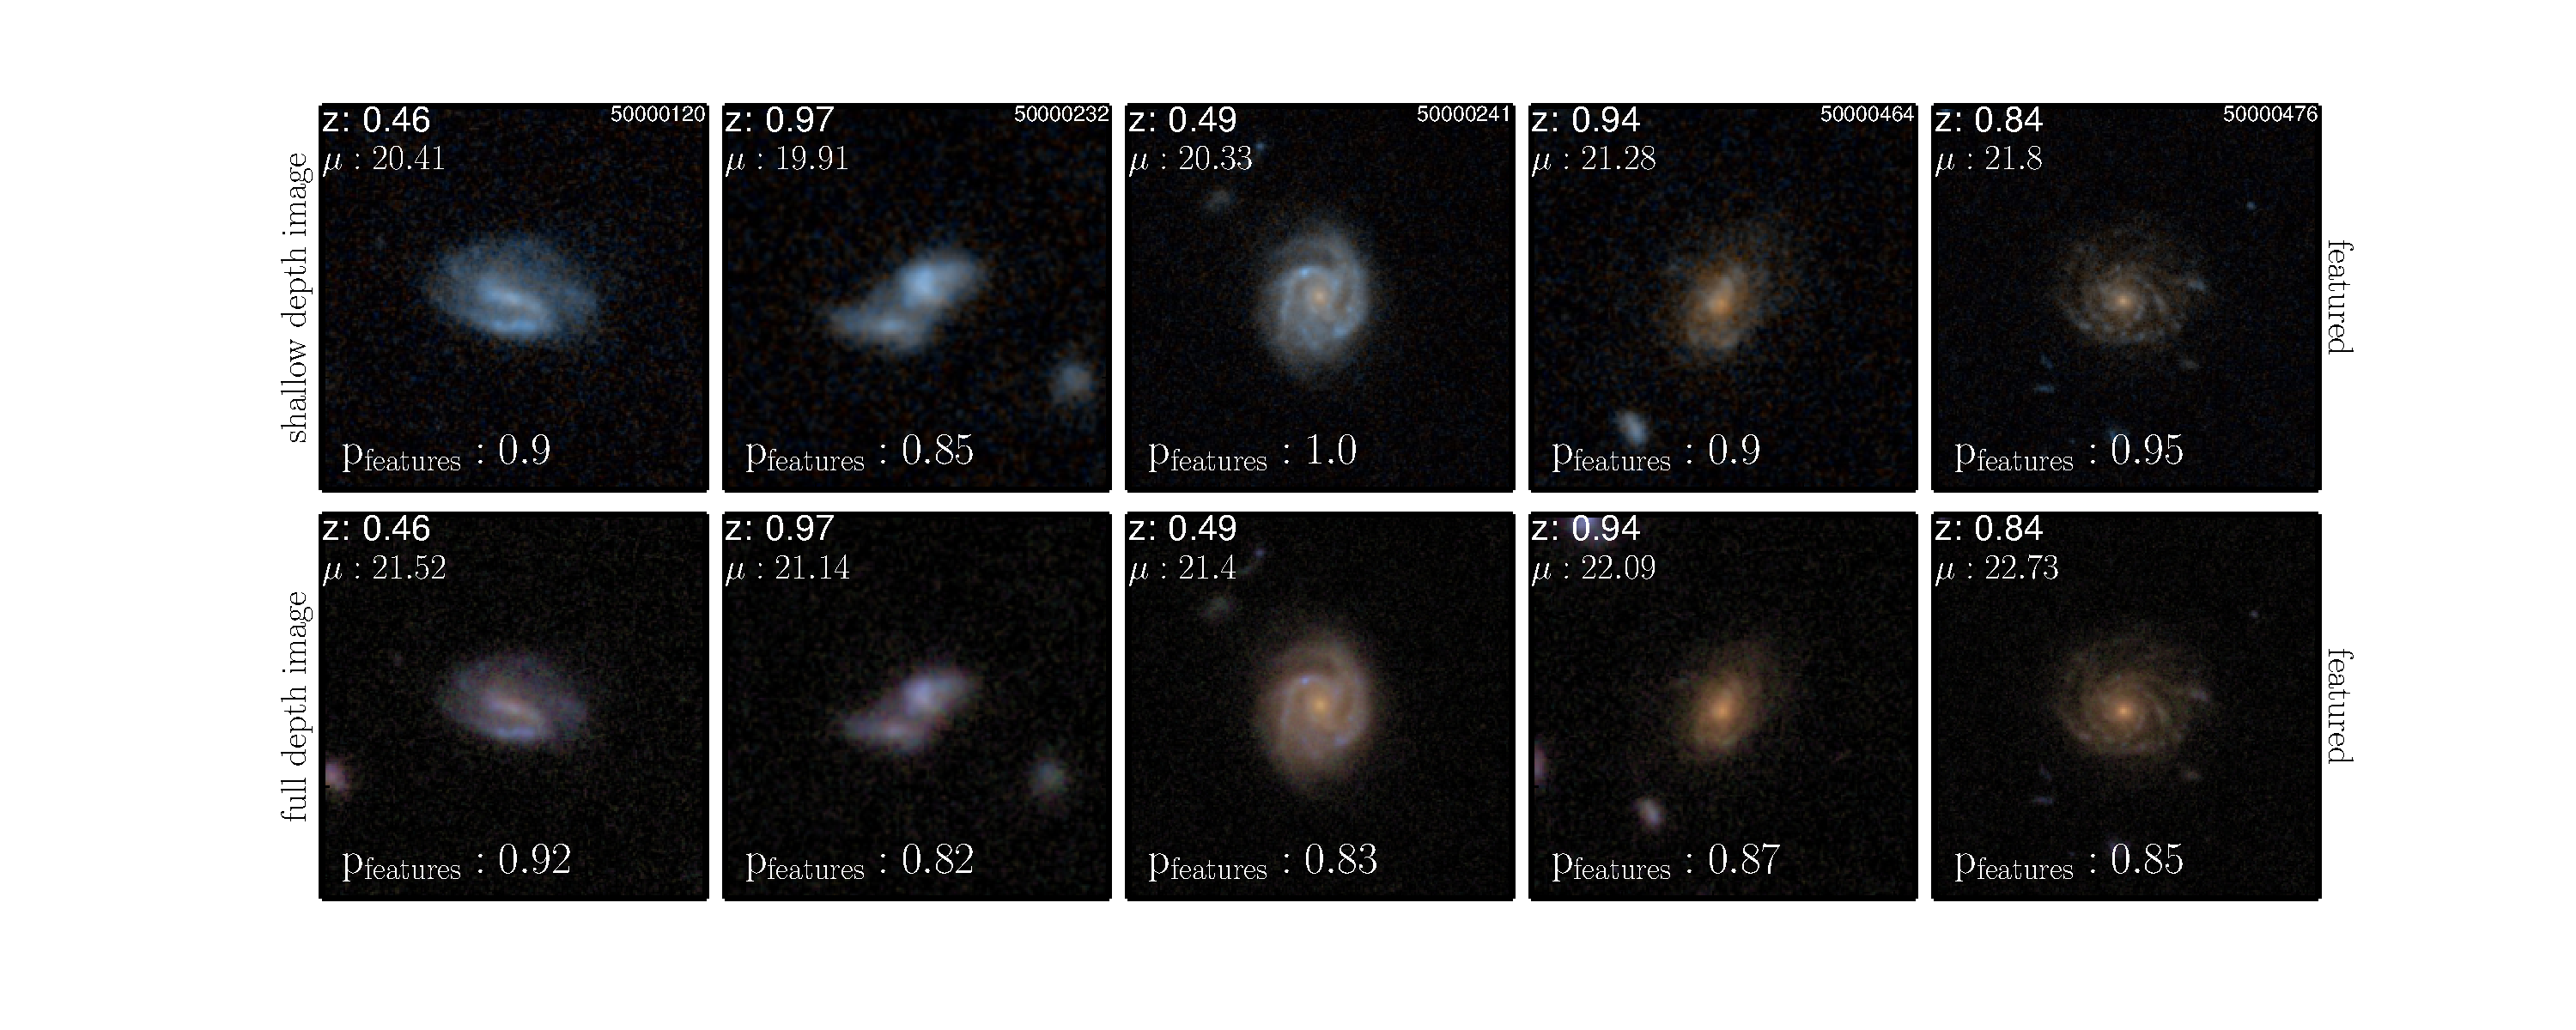
\includegraphics[width=\textwidth]{figures/featured_to_featured.pdf}}


\caption{Galaxies whose shallow images were classified as featured and full depth images were classified as smooth, intermediate, or featured.}
\label{fig:shallow_featured}
\end{figure*}

\subsection{FERENGI analysis of pbar}
\label{sec:ferengi_bar}
\begin{figure*}
\centering
\subfigure{[a]\label{a}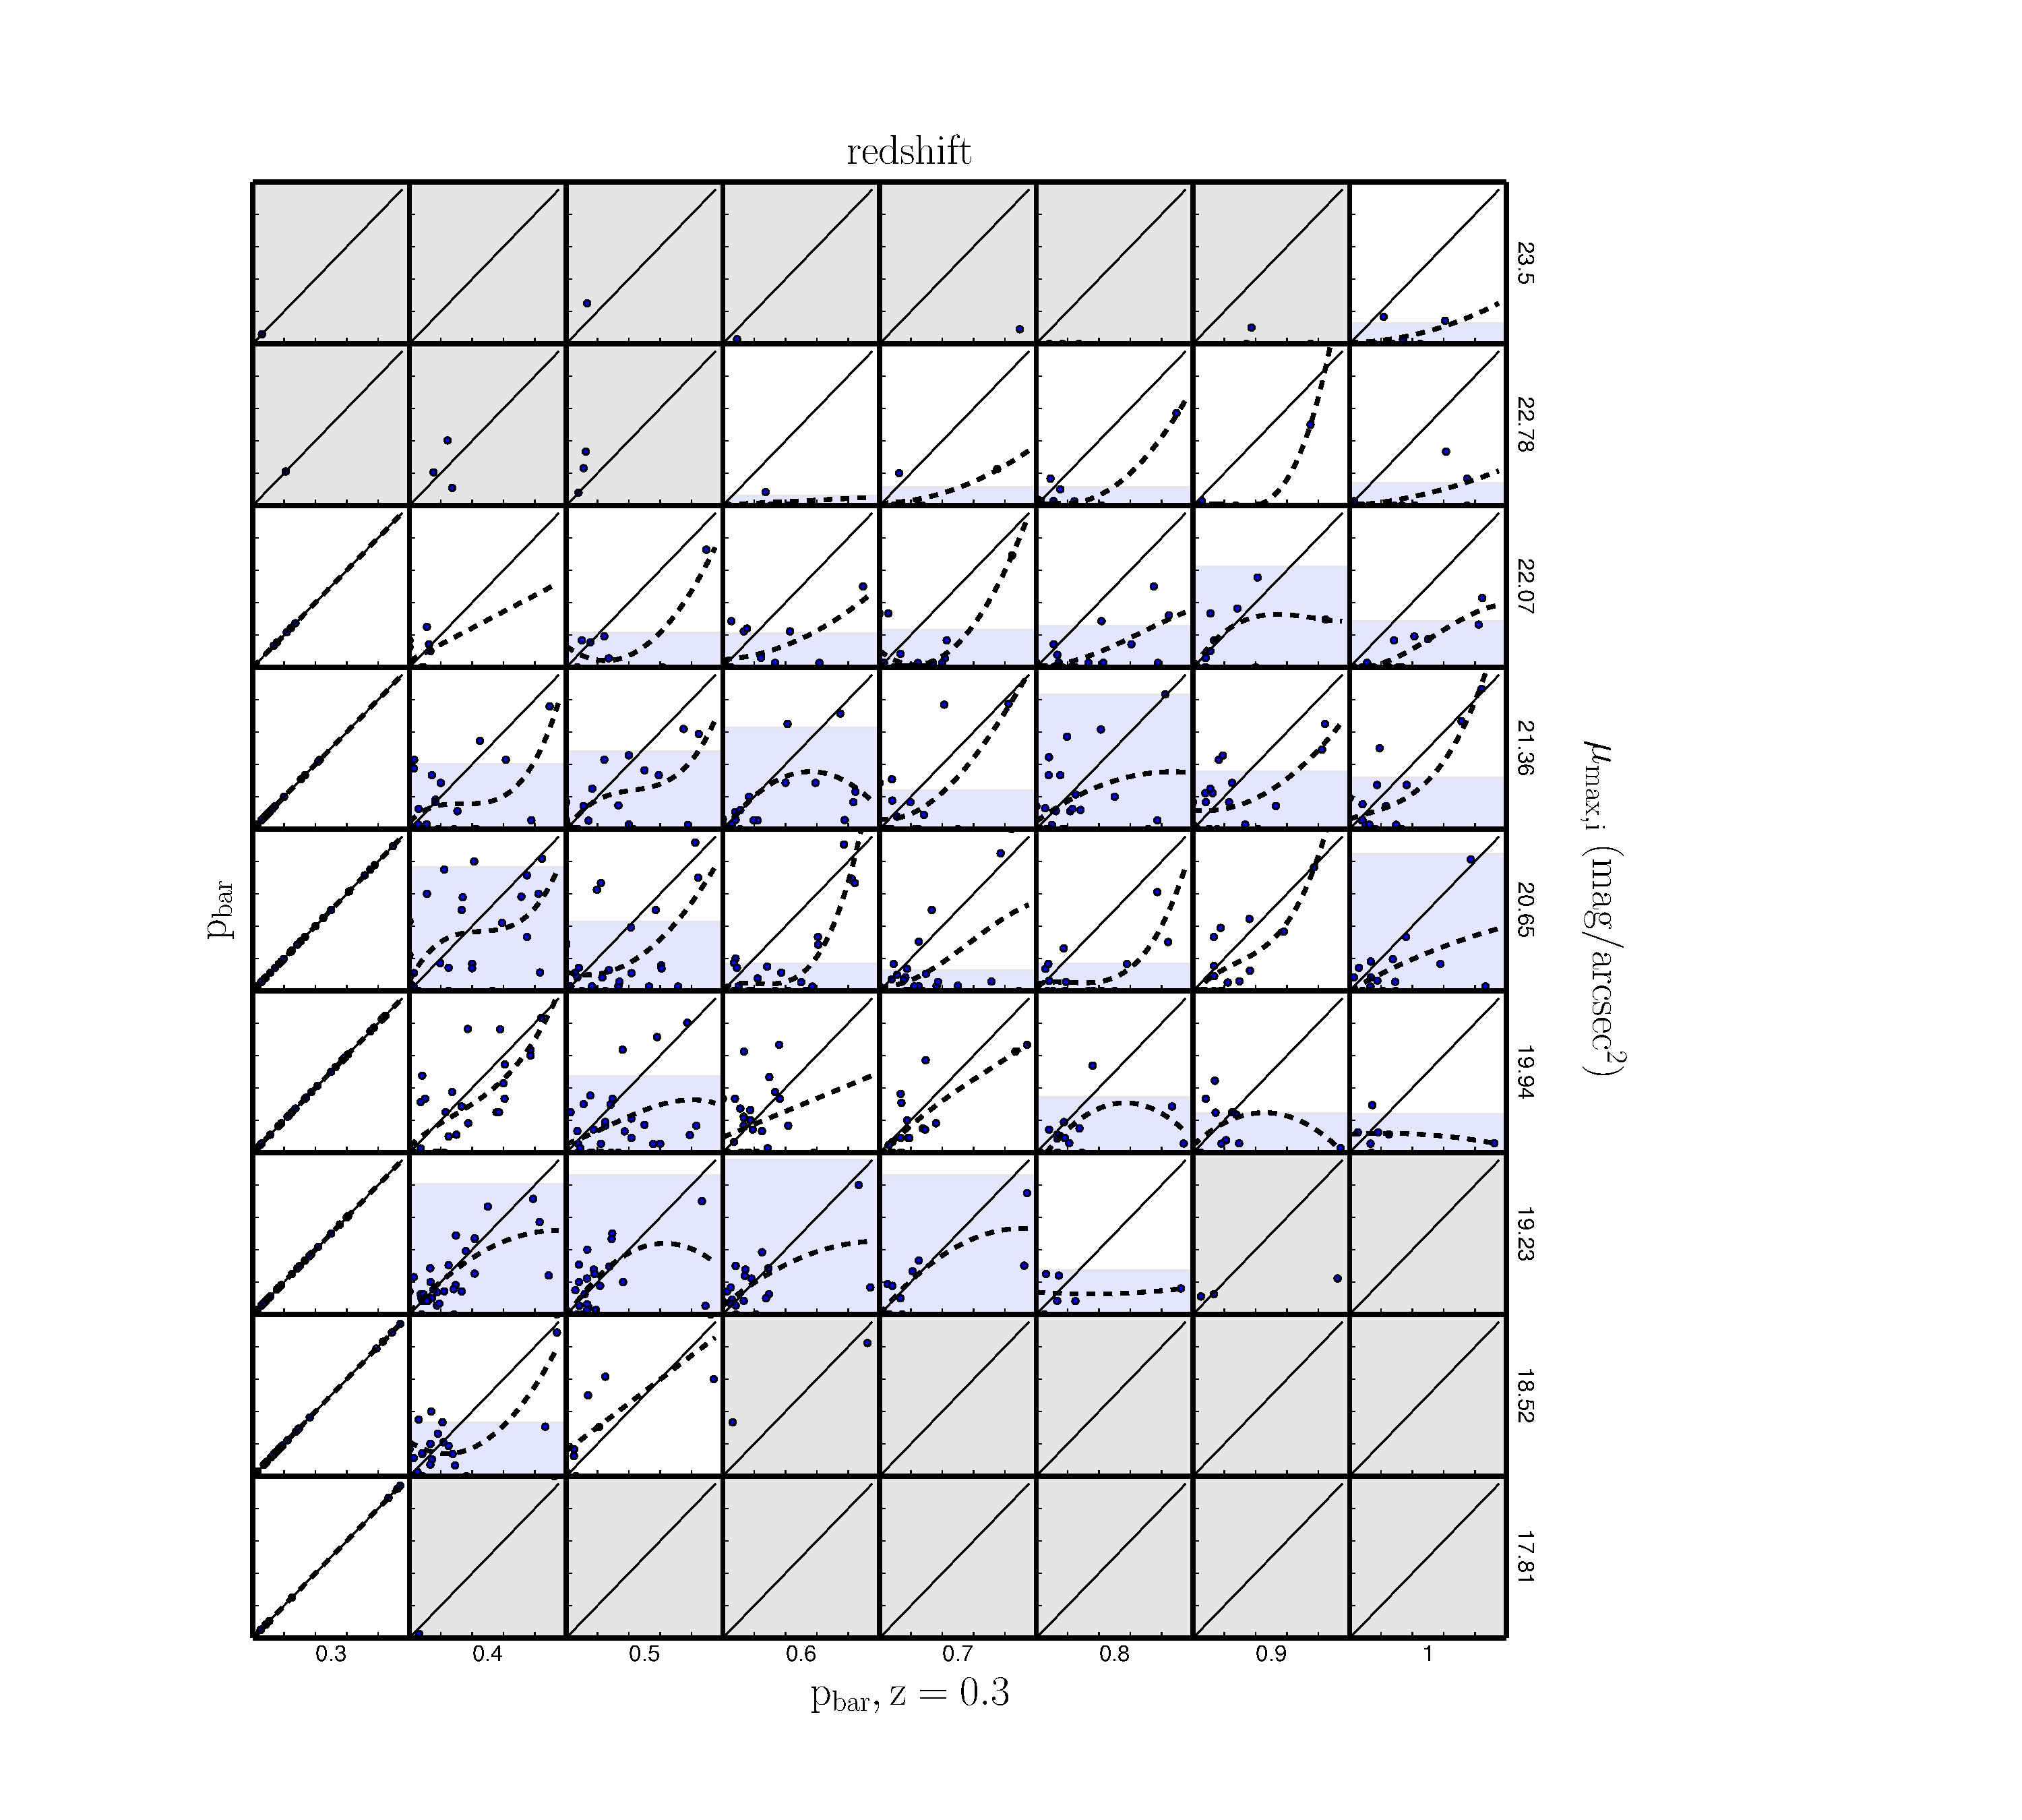
\includegraphics[width=0.5\textwidth]{figures/p_vs_p_SB_redshift_bar.pdf}}
\subfigure{[b]\label{b}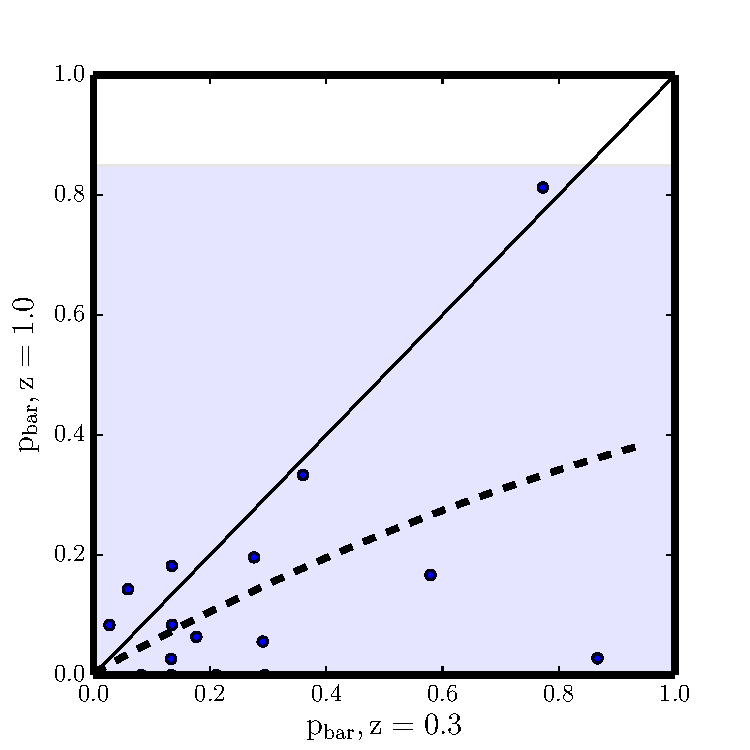
\includegraphics[width=0.4\textwidth]{figures/z1_mu20_subplot1_bar.pdf}}
\\
\subfigure{[c]\label{c}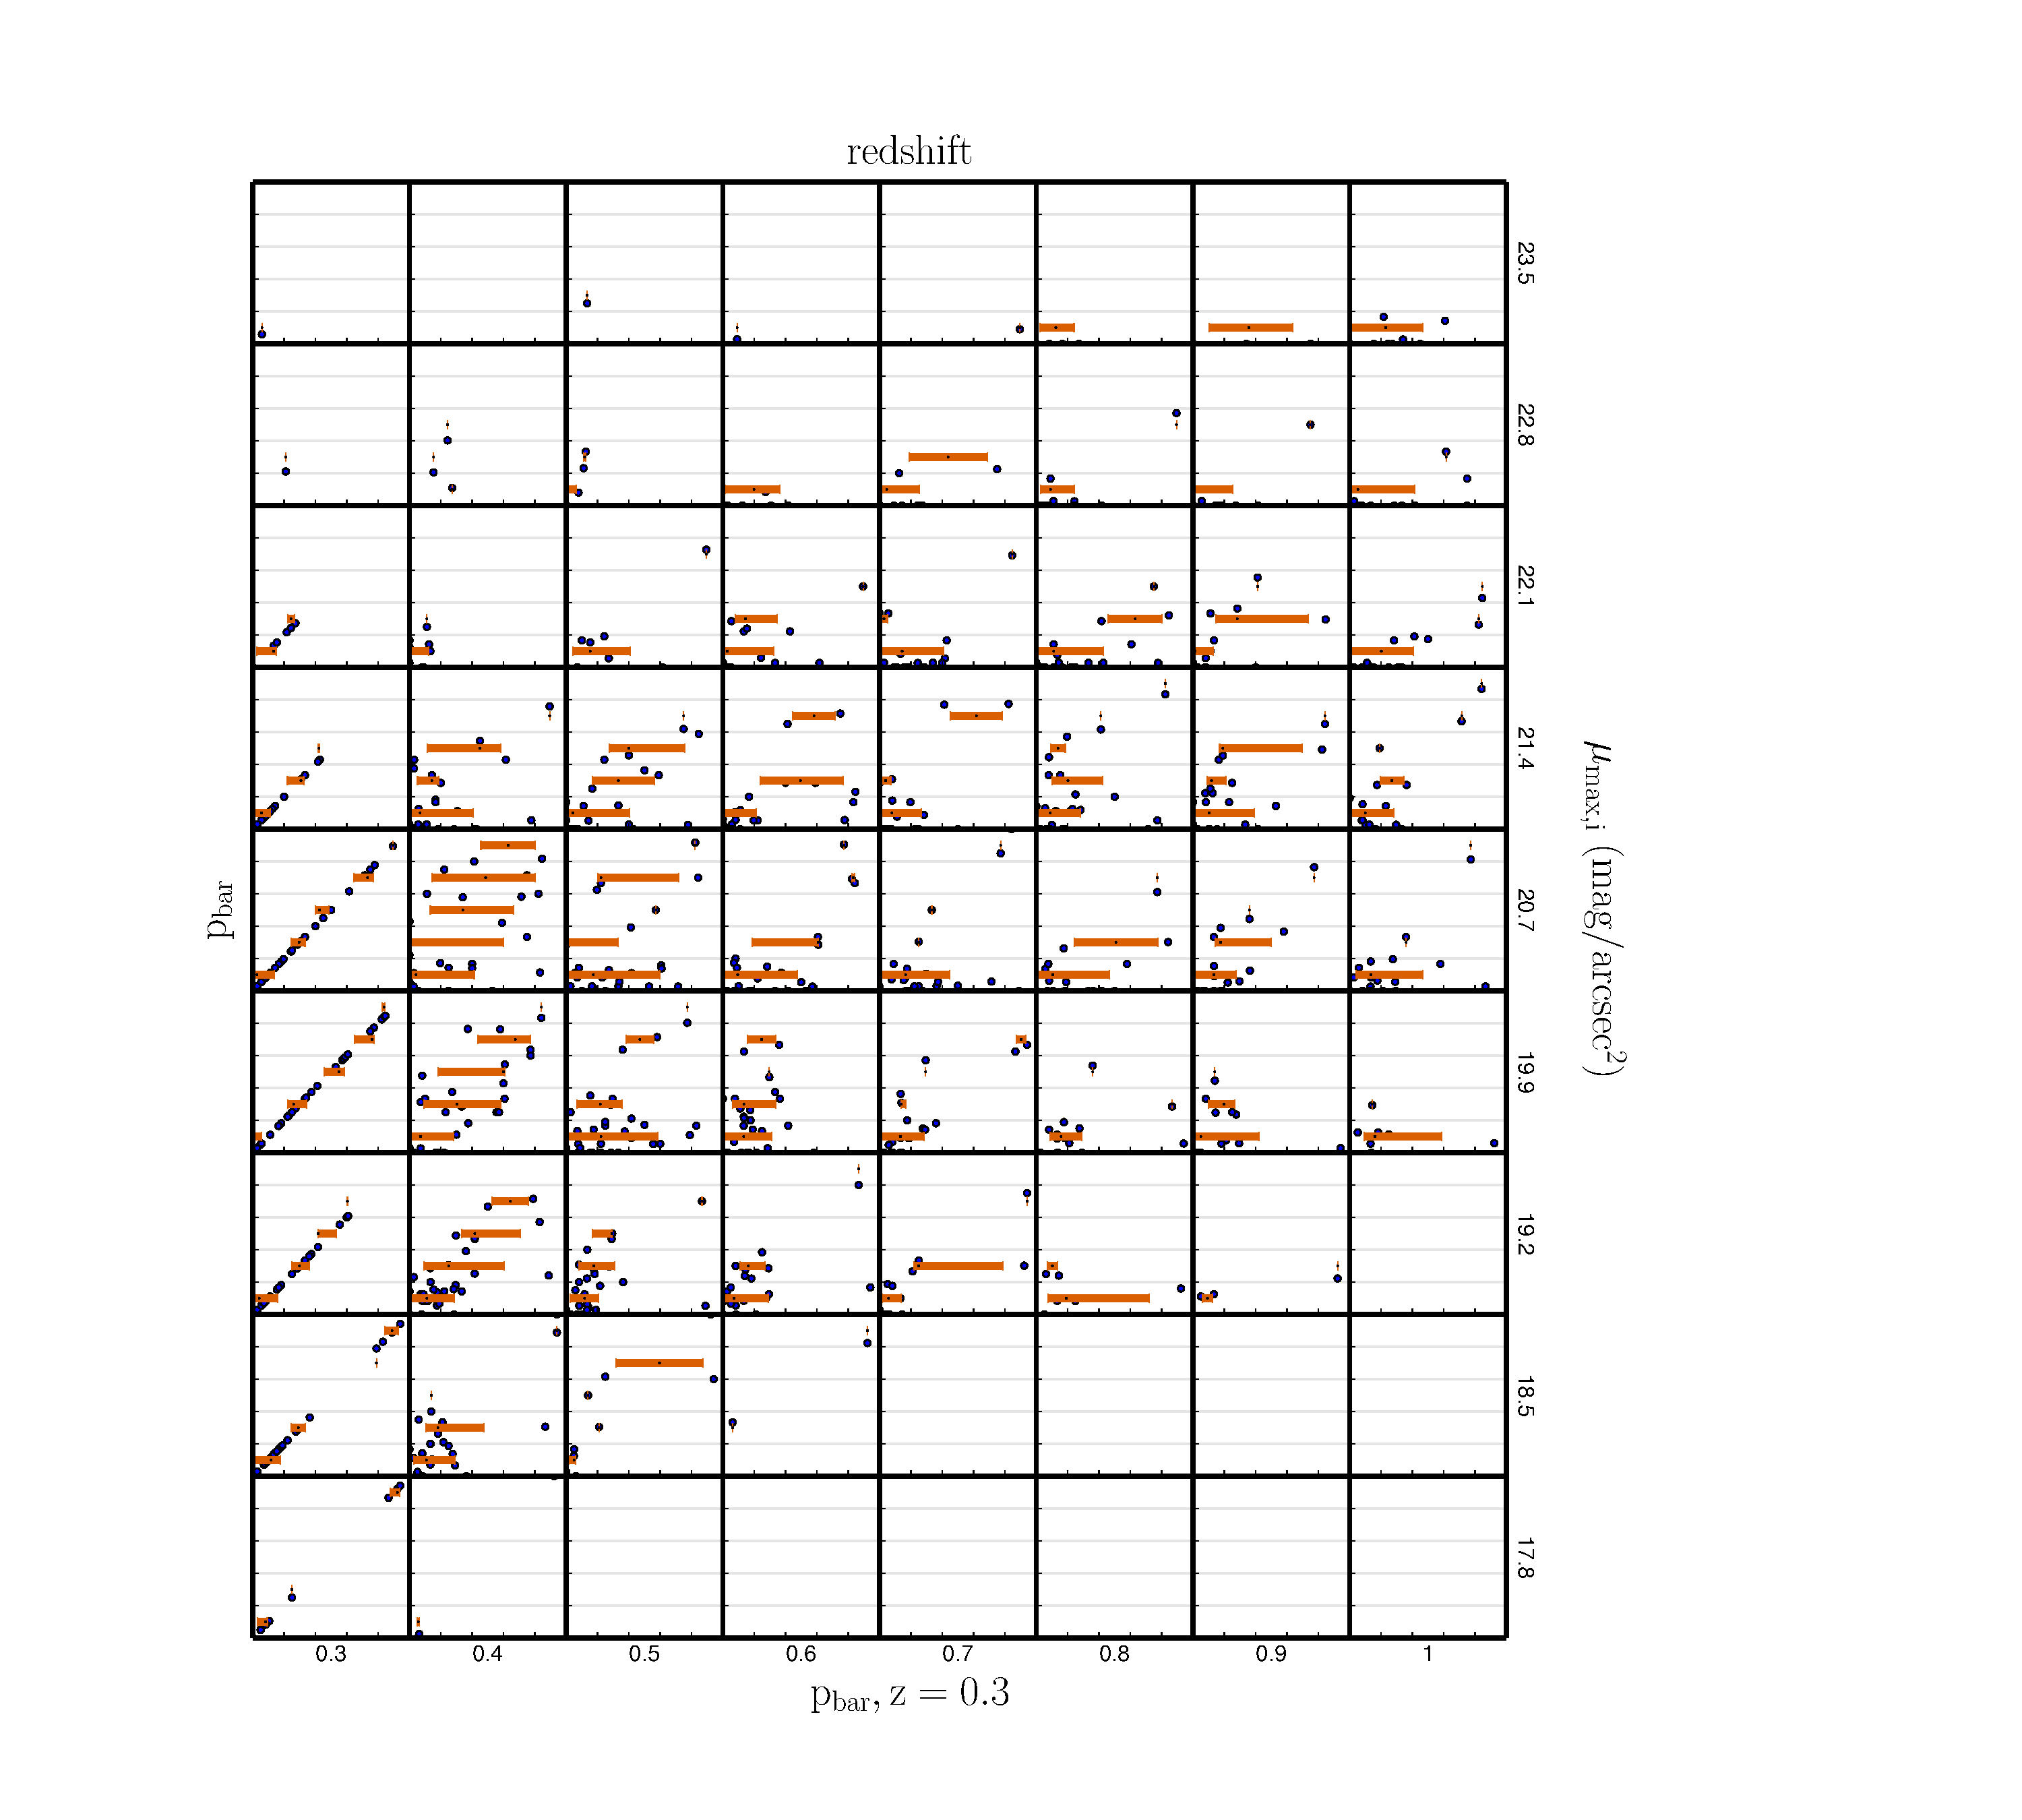
\includegraphics[width=0.5\textwidth]{figures/orangebars_bar.pdf}}
\subfigure{[d]\label{d}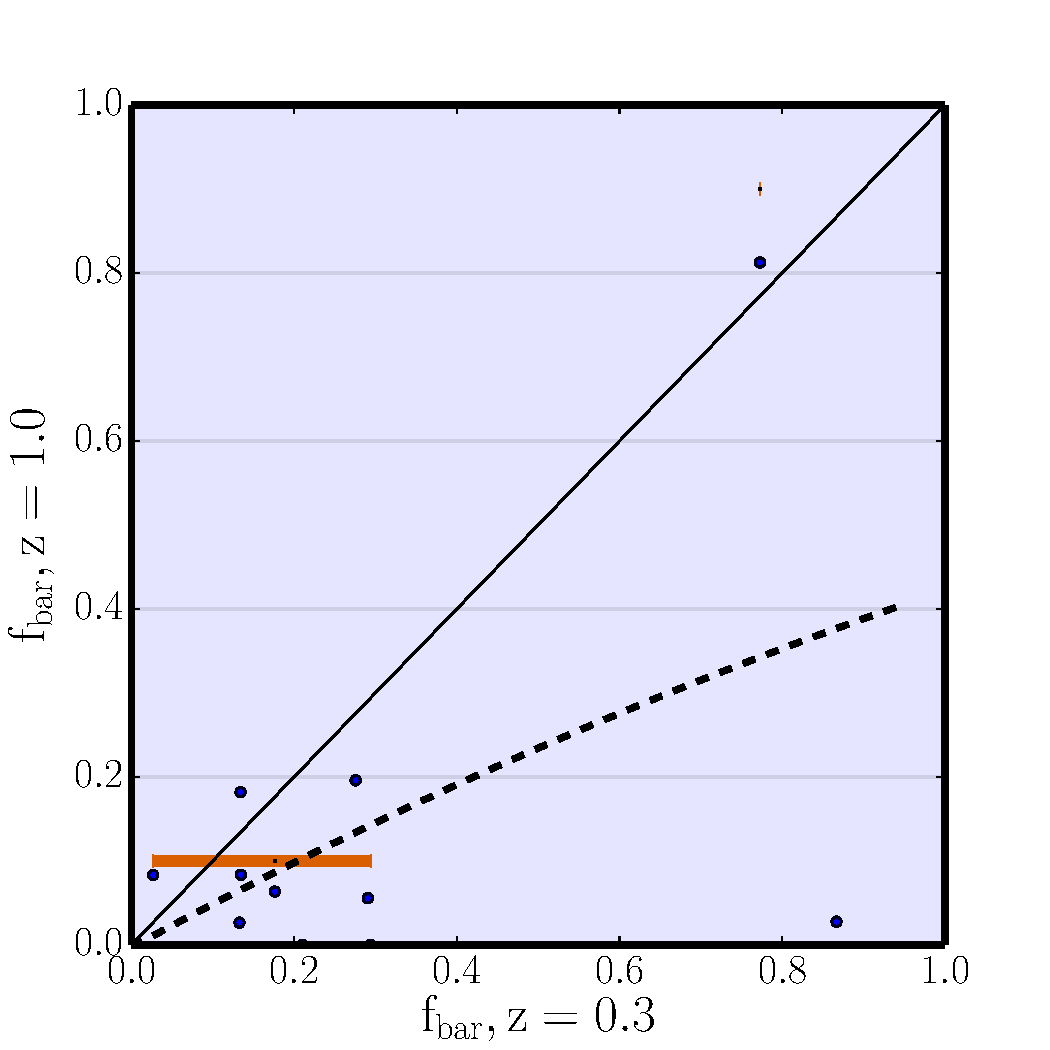
\includegraphics[width=0.4\textwidth]{figures/z1_mu20_subplot2_bar.pdf}}
\caption{Same as Figure~\ref{fig:p_vs_p}, but with the bar question.}
\label{fig:p_vs_p_bar}
\end{figure*}

\begin{table}ー
\caption{Distribution of \ferengi{} images analysed in Figure~\ref{fig:p_vs_p_bar}. Correctable images had a single-valued relationship between their measured $p_{\rm bar}$ values at high and low redshifts (white regions in Figure~\ref{fig:p_vs_p_bar}). Uncorrectable images had a non single-valued relationship (blue regions). NEI images had undetermined relationships due to a lack of data ($N<5$) in their corresponding z-$\mu$ bins (gray regions). Only 17\% (maximum) of FERENGI galaxies in the sample were considered ``correctable'', which is not sufficient to compute a $\zeta$ function applicable to the Hubble data.   \label{ferengi_bar_corrections}}
\begin{tabular}{lrr}
\hline \hline
				                   & N       & \% \\
\hline 
Correctable                        & 664   & 17\% \\
Uncorrectable                      & 483   & 12\% \\
NEI                                & 2,803     & 71\%\\
Total                              & 3,950   & 100\% \\
\hline \hline
\end{tabular}
\end{table}


\end{document}
